\documentclass[a4paper, twoside]{report}
\setcounter{secnumdepth}{5}
\usepackage[utf8]{inputenc}
\usepackage{graphicx}
\graphicspath{ {images/} }
\usepackage[a4paper,width=150mm,top=25mm,bottom=25mm,bindingoffset=6mm]{geometry}
\usepackage{fancyhdr}
\usepackage{listings}
\usepackage{csquotes}
\usepackage{quoting}
\pagestyle{fancy}
\fancyhead{}
\fancyhead[RO,LE]{
    {Auditoría de Software Orientada a Compiladores.
    Caso de Estudio: Solidity}
}
\fancyfoot{}
\fancyfoot[LE,RO]{\thepage}
\fancyfoot[LO,CE]{Chapter \thechapter}
\fancyfoot[CO,RE]{Matías A. Ré Medina}
\renewcommand{\headrulewidth}{0.4pt}
\renewcommand{\footrulewidth}{0.4pt}

% Copyright 2017 Sergei Tikhomirov, MIT License
% https://github.com/s-tikhomirov/solidity-latex-highlighting/

\usepackage{listings, xcolor}

\definecolor{verylightgray}{rgb}{.97,.97,.97}

\lstdefinelanguage{Solidity}{
	keywords=[1]{anonymous, assembly, assert, balance, break, call, callcode, case, catch, class, constant, continue, contract, debugger, default, delegatecall, delete, do, else, event, export, external, false, finally, for, function, gas, if, implements, import, in, indexed, instanceof, interface, internal, is, length, library, log0, log1, log2, log3, log4, memory, modifier, new, payable, pragma, private, protected, public, pure, push, require, return, returns, revert, selfdestruct, send, storage, struct, suicide, super, switch, then, this, throw, transfer, true, try, typeof, using, value, view, while, with, addmod, ecrecover, keccak256, mulmod, ripemd160, sha256, sha3}, % generic keywords including crypto operations
	keywordstyle=[1]\color{blue}\bfseries,
	keywords=[2]{address, bool, byte, bytes, bytes1, bytes2, bytes3, bytes4, bytes5, bytes6, bytes7, bytes8, bytes9, bytes10, bytes11, bytes12, bytes13, bytes14, bytes15, bytes16, bytes17, bytes18, bytes19, bytes20, bytes21, bytes22, bytes23, bytes24, bytes25, bytes26, bytes27, bytes28, bytes29, bytes30, bytes31, bytes32, enum, int, int8, int16, int24, int32, int40, int48, int56, int64, int72, int80, int88, int96, int104, int112, int120, int128, int136, int144, int152, int160, int168, int176, int184, int192, int200, int208, int216, int224, int232, int240, int248, int256, mapping, string, uint, uint8, uint16, uint24, uint32, uint40, uint48, uint56, uint64, uint72, uint80, uint88, uint96, uint104, uint112, uint120, uint128, uint136, uint144, uint152, uint160, uint168, uint176, uint184, uint192, uint200, uint208, uint216, uint224, uint232, uint240, uint248, uint256, var, void, ether, finney, szabo, wei, days, hours, minutes, seconds, weeks, years},	% types; money and time units
	keywordstyle=[2]\color{teal}\bfseries,
	keywords=[3]{block, blockhash, coinbase, difficulty, gaslimit, number, timestamp, msg, data, gas, sender, sig, value, now, tx, gasprice, origin},	% environment variables
	keywordstyle=[3]\color{violet}\bfseries,
	identifierstyle=\color{black},
	sensitive=false,
	comment=[l]{//},
	morecomment=[s]{/*}{*/},
	commentstyle=\color{gray}\ttfamily,
	stringstyle=\color{red}\ttfamily,
	morestring=[b]',
	morestring=[b]"
}

\lstset{
	language=Solidity,
	backgroundcolor=\color{verylightgray},
	extendedchars=true,
	basicstyle=\footnotesize\ttfamily,
	showstringspaces=false,
	showspaces=false,
	numbers=left,
	numberstyle=\footnotesize,
	numbersep=9pt,
	tabsize=2,
	breaklines=true,
	showtabs=false,
	captionpos=b
}


\usepackage{tcolorbox}
\newtcolorbox{notesBox}{colback=gray!5!white,colframe=gray!75!black}

\usepackage[backend=biber,style=authoryear,sorting=ynt,style=numeric-comp]{biblatex}
\addbibresource{./references.bib}
\begin{document}

\begin{titlepage}
    \begin{center}
        \vspace*{1cm}
 
        \Large
        \textbf{Auditoría de Software Orientada a Compiladores}
 
        \vspace{0.3cm}
        \Large
        {Caso de Estudio: Solidity}
 
        \vspace{1.5cm}
        
        \large
        \textbf{{Matías Ariel Ré Medina}\\
        {Dr. Ing. José María Massa}
        }
 
        \vfill
 
        Una tésis presentada para el título de\\
        Ingeniería en Sistemas
 
        \vspace{0.8cm}
 
        {
\includegraphics[height=258px,width=300px]{unicen_big.jpg}}
        \vspace*{0.3cm}

        \large
        Ciencias Exactas\\
        UNICEN\\
        Argentina\\
        Diciembre 2019
 
    \end{center}
\end{titlepage}

% \thispagestyle{plain}
\begin{center}
    \Large
    \textbf{Auditoría de Software Orientada a Compiladores}

    \vspace{0.2cm}
    \large
    {Caso de Estudio: Solidity}
 
    \vspace{0.4cm}
    \textbf{{Matías Ariel Ré Medina}\\
    {Dr. Ing. José María Massa}
    }
 
    \vspace{0.9cm}
    \textbf{Abstract}
\end{center}

Lorem ipsum dolor sit amet, consectetur adipiscing elit. Vestibulum tincidunt est et quam aliquam, sit amet fermentum dui tincidunt. Donec fringilla ipsum fermentum nibh ultrices mattis. Sed eu metus ultricies, malesuada diam pulvinar, lacinia velit. Sed maximus justo eget mi aliquam vestibulum. Mauris eget magna id risus sodales ullamcorper non sed orci. Orci varius natoque penatibus et magnis dis parturient montes, nascetur ridiculus mus. Suspendisse egestas augue in volutpat tincidunt. Vivamus ac urna finibus, imperdiet enim quis, elementum odio. Phasellus vel pretium ipsum. Morbi non ipsum convallis, consectetur nisi vitae, tempus sem. Fusce sodales, augue vitae posuere dignissim, odio nibh volutpat enim, sed placerat risus elit quis mi. Ut pretium convallis tellus, at faucibus nulla. Aliquam porta neque in orci vehicula, eu ultrices nunc consequat. Suspendisse sodales diam sit amet nisi luctus, eget ullamcorper elit consectetur. Curabitur nec libero velit.

Praesent ligula mi, convallis eget turpis eu, tempor faucibus nunc. Praesent consequat tortor ac ligula dapibus ultricies. Duis id accumsan metus. Phasellus vel diam in velit dignissim vulputate. Integer sodales ullamcorper lorem eget suscipit. Phasellus gravida tempus facilisis. Sed mi sem, convallis posuere elit in, aliquam laoreet tellus. Etiam finibus feugiat purus, gravida condimentum sapien maximus a. Pellentesque ac risus turpis. Sed a nibh diam. Etiam viverra nisl auctor nulla efficitur fringilla. Vivamus vitae arcu a ante lobortis ullamcorper. Proin et lorem consectetur, aliquet nisi ac, tempus sem. Aenean ut massa id eros efficitur tincidunt.

Nam eu condimentum sem. Etiam iaculis et nunc a sollicitudin. Nulla vitae quam magna. Aliquam vestibulum, nibh ut accumsan malesuada, libero est facilisis ante, in aliquet mi velit quis nibh. Suspendisse pharetra sapien vitae massa sodales fringilla. Sed varius nulla eget lorem dignissim lacinia. Phasellus hendrerit imperdiet magna id hendrerit. Curabitur porttitor leo nec luctus tempus. Maecenas hendrerit, mauris ac auctor tempor, magna nulla accumsan mi, et dictum quam tellus a nunc. Etiam auctor dui ut lectus maximus, sed accumsan nunc facilisis.
 
% \chapter*{Dedicación}
% Quiero dedicarle la tésis particularmente a mis padres, en principal a mi madre Silvia Medina.
 
% \chapter*{Agradecimientos}
% Me gustaría agradecerle a los que me acompañaron a lo largo de las investigaciones
% que desarrollé, dentro de mi inconformidad, hasta dar con esta que terminaría siendo mi tésis.
% Sebastián Fernández, Patricio Palladino, Iñaki Berra, Mariano Cocirio, Coni, Viole.
 
\tableofcontents


% \chapter{Introducción}
% \section{Prólogo}
Considerando que el mundo de la tecnología informática es un campo relativamente nuevo, que día a día crece exponencialmente, hay que destacar que dentro de él también se encuentran campos como el de la \textit{seguridad informática}, que son mucho más recientes.\\

La explotación de vulnerabilidades existentes y nuevas permite el acceso no autorizado a los bienes de una empresa, siendo un problema de seguridad de alta gravedad. \textit{Una gran proporción de todos los incidentes de seguridad de software son causados por atacantes que explotan vulnerabilidades conocidas.}\cite{sectesting}

\begin{displayquote}
\textit{``Romper algo es más fácil que diseñar algo que no se puede romper."}
\newline{\null\hfill -- Gary McGraw}
\end{displayquote}

Por eso es fundamental que se realice la comprobación de las aplicaciones, redes, sistemas nuevos y ya presentes, en búsqueda de vulnerabilidades para asegurarse que nadie sin acceso autorizado haya accedido previamente ni lo haga en el futuro.\\

Los análisis de seguridad comúnmente no llegan a cubrir el total de la infraestructura de una empresa. Hay dos principales razones por las cuales esto sucede: la inmensidad de las mismas y los plazos breves de tiempo disponibles para el trabajo\cite{krypsys}\cite{specopssoft}\cite{crest}\cite{notsosecure}. No obstante, los mecanismos utilizados son efectivos, lo suficiente como para identificar vulnerabilidades conocidas, y comprobar cómo un atacante podría acceder a sus sistemas.\\

Las técnicas de testeo empleadas en el ciclo de vida del desarrollo seguro de un software se pueden distinguir en cuatro categorías: \textbf{(1)} \textit{pruebas de seguridad basadas en modelos que se basan en los requisitos y los modelos de diseño creados durante la fase de análisis y diseño}, \textbf{(2)} \textit{pruebas basadas en código y análisis estático en el código fuente y bytecode creado durante el desarrollo}, \textbf{(3)} \textit{pruebas de penetración y análisis dinámico en sistemas en ejecución, ya sea en un entorno de prueba o producción}, así como \textbf{(4)} \textit{pruebas de regresión de seguridad realizadas durante el mantenimiento}\cite{sectesting}. A pesar de que algunos mecanismos eran utilizados específicamente en el mundo de la seguridad informática, \textit{dejando de lado la revisión de código por supuesto}, desarrolladores y DevOps están utilizando cada vez más estrategias como \textit{fuzzing y análisis estático de código} para probar la calidad de su software\cite{accelerate_report}\cite{concepts}.

\section{Motivación}
En las carreras universitarias las cuestiones de seguridad no se tratan con profundidad y de una manera enfocada al problema, sino desde los aspectos subyacentes que permiten entender los problemas de seguridad y sus posibles soluciones.  Es por ello que los graduados que decidan dedicarse a la seguridad informática, deben especializarse por su cuenta a través de cursos, o mediante el aprendizaje profesional que se da a través de la resolución de problemáticas de los clientes.\\

Esta propuesta surge por un interés personal originado gracias a las materias \textit{Lenguajes de Programación y Diseño de Compiladores}, y al incremento que ha habido últimamente en desarrollo de nuevos lenguajes, que poseen propósitos y contextos distintos\cite{Klabnik:2018:RPL:3271463}\cite{Forsgren:2018:ASL:3235404}.

\subsection{Contexto}
Los \textit{Smart Contracts}, son programas que poseen una ejecución completamente verificable y observable. Esto permite que exista la certeza de que la ejecución del mismo no pueda ser alterada, abriendo una nueva posibilidad de casos de usos que en las plataformas de cómputo tradicionales no existían.\\

\textit{Ethereum Network} fue desarrollada para ser una plataforma de \texttt{smart contracts}, siendo la primera que posee un lenguaje (del estilo bytecode) con característica \textit{Turing complete} (permite que un el lenguaje pueda llegar a programarse para realizar cualquier tipo de operación) que corre en una máquina virtual llamada \textit{Ethereum Virtual Machine (EVM)}.\\

Si bien hay diversos lenguajes de programación que son compilados a la representación en bytecode para EVM, el que es oficialmente desarrollado y posee financiación por parte de la \textit{Ethereum Foundation} es \textbf{Solidity}\cite{solidity_readthedocs}.\\

\texttt{Solidity}, que si bien se puede percibir como un lenguaje medianamente similar a \texttt{Javascript} en cuanto a sus aspectos sintácticos y en menor medida semánticos, nació de la necesidad de tener un lenguaje de alto nivel orientado a desarrollar \textit{Smart Contracts} que permita interactuar con la \texttt{Ethereum Network}. \\

Los \texttt{smart contracts} hoy en día manipulan y almacenan caudales de dinero de gran magnitud, es por eso que es inevitable que la seguridad en estos casos se haga presente.\\

Ha habido ya muchos casos registrados de pérdidas de miles de millones de dólares, debido a descuidos a la hora de desarrollar y por no entender este muy reciente \textit{“paradigma”}:
\begin{itemize}
\item Uno de los clientes más populares utilizado para facilitar a los usuarios la interacción con la red, congeló fondos valuados en \$100 millones de dólares debido a un error en su código\cite{Hertig:Alyssa:Coindesk}.
\item En julio del 2017, días después de que un hacker obtuviera más de 7 millones de dólares explotando una vulnerabilidad, debido a otro error en el mismo cliente, otro hacker obtuvo acceso a fondos de algunas cuentas, valuado en un total de \$37 millones de dólares \cite{Pearson:Jordan:Motherboard}.
\item Un ejemplo de un error de diseño del lenguaje con impacto a gran escala es el caso del famoso llamado, en este ambiente, \texttt{reentrancy bug}. Permitía a un atacante retirar una gran cantidad de veces su balance de un contrato, volviendo a llamar a la misma funcionalidad en medio de su ejecución, logrando así multiplicar sus fondos\cite{Vessenes:Peter:Vessenes}.
\end{itemize}
\bigskip

Así es como que desde el lado de los estudios de los lenguajes de programación, parece de suma relevancia poseer lenguajes y compiladores correspondientes que funcionen de manera esperada, sin permitirle a los desarrolladores la posibilidad de cometer errores catastróficos.\\

En este contexto un error en la generación del bytecode podría detener el funcionamiento de una red de miles de máquinas virtuales, o financieramente impactar de formas inesperadas en el contrato desarrollado.

\section{Objetivos}
\textit{Realizar una investigación de las estrategias y metodologías existentes para auditar compiladores, brindando primero una introducción a la auditoría de software, luego una introducción a auditoría específicamente de compiladores, comentando las técnicas más populares.}\\

\textit{Finalmente evaluar como caso de uso una auditoría al lenguaje \textbf{Solidity} y a su compilador \textbf{solc}, explicando el proceso y herramientas utilizadas, mostrando los resultados obtenidos.}

% \chapter{Marco teórico}
% En esta sección se presentarán los conceptos teóricos subyacentes en los que está basado este trabajo de investigación, que se utilizan a lo largo de este documento y son la base para comprender el marco en torno a él.

En la las primeras secciones, 2.1 a 2.6, se habla de las distintas estrategias, metodologías, y técnicas que envuelven el proceso de auditar un software. En las secciones 2.7 y 2.8 se introduce al compilador como un pilar importante en el proceso del desarrollo de software, y se explica su anatomía. Por último, en la secciones 2.9, 2.10 y 2.11, se presenta el concepto de una estructura blockchain, los smart contracts, y el lenguaje de interés Solidity, quién posee su propio compilador como parte del proceso de su utilización.


\section{Auditoría de software (seguridad)}
Uno de los \textit{aclamados} padres de la seguridad informática del software, comenzó preguntándose por qué los creadores de Java fallaron al aplicarle seguridad al lenguaje en su momento. Buscando sobre cómo aprender sobre ello, se descubrió para su sorpresa que hasta ese momento ningún libro se había escrito al respecto, siendo que se sitúa a mediados de los 90'.

Luego de eso, en el 2000 publicó un libro llamado \textbf{Building Secure Software} (construyendo software seguro), junto a John Viega, que terminó siendo el \textit{primer libro} en el mundo relacionado a seguridad en software.

Desde entonces se han publicado muchos otros libros\cite{McGraw:2006:SSB:1121680}\cite{Shostack:2014:TMD:2829295}\cite{Hoglund:2004:ESB:984253}\cite{Howard:2009:DSS:1594832}\cite{Klein:2011:BHD:2823924}\cite{Allen:2008:SSE:1386212}\cite{Wysopal:2006:ASS:1196390}\cite{Ransome:2013:CSS:2613389}, y se han aplicado estándares como \textbf{Building Security In Maturity Model}\cite{McGraw:2015:SSB:2675327.2675329} (BSIMM, al estilo CMMI que ahora es el estándar de facto para medir iniciativas de seguridad de software), así como también el \textbf{Estándar de Verificación en Seguridad de Aplicaciones}\cite{OWASP:AVSP} (ASVS de OWASP) y su versión abierta del \textbf{Software Assurance Maturity Model} (Modelo de Madurez de la Seguridad del Software) llamado \textbf{OpenSAMM}\cite{OWASP:OpenSAMM}.

Sin embargo, la mayoría de los artículos que se pueden encontrar relacionados acerca de la seguridad en software comienzan describiendo políticas robustas previo al desarrollo del producto, y desde allí avanzan implementando mejores prácticas y programación segura. El gran problema de ello es que no todos los sistemas que quieran incorporar seguridad hoy en día pueden aplicar esta estrategia, ya que por cuestiones de recursos, o incluso sentido común, no se justificaría comenzar el desarrollo íntegramente desde cero. Es por eso que soluciones como estas sólo tienden a evitar las vulnerabilidades y no tratar las posibles ya existentes, para proyectos que ya estén creados.

Si bien ha habido un gran incremento en la aplicación de seguridad a la hora de desarrollar un software, no existen muchos materiales que traten la búsqueda de vulnerabilidades.

\begin{notesBox}
\textbf{Vulnerabilidad de software versus bug}

Entendiendo el término bug como un error, equivocación, o descuidos en programas que resultan en comportamientos inesperados y no deseados, una vulnerabilidad es un bug con implicancias en seguridad, permitiendo a un atacante abusar de ella para obtener alguna especie de beneficio, ya sea conseguir accesos privilegiados, provocar la caída de un servicio, tomar el control de un sistema o adquirir información sensible. Utilizar esa falla para violar las políticas de seguridad de un proyecto es lo que se llama explotar una vulnerabilidad, y quién intenta explotarla es llamado atacante.
\end{notesBox}

\section{Auditando}
Auditar una aplicación es el proceso de analizar su código (en el formato de su fuente o binario) para descubrir vulnerabilidades que algunos atacantes podrían explotar. Realizando este proceso, se pueden identificar y cerrar agujeros de seguridad que de otra manera pondrían en un riesgo innecesario datos sensibles y recursos de negocios.

El contenido de la presente sección está desarrollado y profundizado en el libro \textit{The Art of Software Security Assessment: Identifying and Preventing Software Vulnerabilities}\cite{Dowd:2006:ASS:1196394} (El arte del asesoramiento de seguridad de software: Identificando y previniendo vulnerabilidades de software).

A continuación ejemplos de algunas situaciones que son de relevancia en las que se realiza una auditoría:\newline

\begin{tabular}{|p{4.3cm}|p{4.3cm}|p{4.3cm}|}
    \hline
    \textbf{Situación} & \textbf{Descripción} & \textbf{Ventaja} \\
    \hline
    Auditoría in-house (pre-release). & Una compañía de software realiza auditorías de código a un nuevo producto antes de su release. & Fallas de diseño e implementación pueden ser identificadas y remediadas antes de que el producto salga al mercado, ahorrando dinero en desarrollo y desplegando actualizaciones. También le ahorra a la compañía una potencial situación vergonzosa. \\
    \hline
    Aditoría in-house (post-release). & Una compañía de software realiza auditorías de código a un nuevo producto luego de su release. & 
    Vulnerabilidades de seguridad pueden ser encontradas y corregidas antes de que partes con intenciones maliciosas las descubran primero. Este proceso permite obtener tiempo para realizar testeos y otros chequeos, al contrario que estar haciendo una publicación en apuros en respuesta a un vulnerability disclosure (la acción de hacer pública una vulnerabilidad). \\
    \hline
    Comparación de productos por terceros. & Un tercero realiza auditorías a varios productos que compiten en un contexto dado. & Un tercero que pueda ser objetivo, puede proveer información útil a consumidores y asistirlos en seleccionar el producto más seguro. \\
    \hline
\end{tabular}
\pagebreak


\begin{tabular}{|p{4.3cm}|p{4.3cm}|p{4.3cm}|}
    \hline
    Evaluación por terceros & Un tercero realiza una auditoría de software de manera independiente para un producto de un cliente. & El cliente puede obtener un gran entendimiento de la seguridad relativa a un producto que pretende desplegar. Esto prueba ser el factor decisivo entre la compra de un producto u otro. \\
    \hline
    Evaluación preliminar por terceros. & Un tercero realiza una auditoría de software de manera independiente de un producto antes de que salga al mercado. & Capitalistas de riesgo pueden obtener una idea de la viabilidad de una futura tecnología con propósitos de financiamiento. Proveedores pueden también realizar este tipo de evaluación para asegurar la calidad de un producto que pretenden llevar al mercado. \\
    \hline
    Investigación independiente. & Una compañía de seguridad o una firma de consultoría realiza una auditoría de software de manera independiente. & Proveedores de productos de seguridad pueden identificar vulnerabilidades e implementar medidas de protección en scanners y otros dispositivos de seguridad. La investigación independiente también funciona como una industria que está atenta y provee una manera para que los investigadores y compañías de seguridad establezcan credibilidad profesional. \\
    \hline
\end{tabular}

\subsection{Auditando versus black box testing}
La idea del black box, o testeo de caja negra, es evaluar un sistema solamente manipulando sus interfaces, en el cual la estructura, el diseño o la implementación interna del objeto que se está analizando no es conocido por el profesional de validación (tester). Es llamado así, porque el software a ojos del tester es como una caja en la cual el contenido no se puede ver.

Desde la perspectiva de seguridad, y no tanto asociado a las definiciones formales, como la que podría proveer a los profesionales informáticos el \textbf{International Software Testing Qualifications Board} (Comité Internacional de Certificaciones de Pruebas de Software), lo que se busca es comunicarse con estas interfaces de maneras inesperadas para la lógica contenida en el software. Es decir, si se está testeando con esta metodología un servidor web (web server), se enviarán variantes de peticiones de protocolo \textbf{HTTP} (Hyper Text Transfer Protocol) reales, malformadas, e incluso modificadas para ser de un tamaño mayor al posiblemente esperado.

Cualquier comportamiento inesperado, o el mero detenimiento del software analizado es considerado algo de gran seriedad. El hecho de automatizar este proceso, para acelerar el hallazgo de más fallas, es llamado \textbf{\textit{fuzz-testing}}, del cual se hablará con profundidad más adelante.

A menudo, analizando código manualmente se pueden encontrar vulnerabilidades que realizando tareas automatizadas probablemente pasen por alto, y es por eso que existe la necesidad de realizar asesoramientos a las estructuras del código de manera inteligente, en adición a simplemente correr herramientas automatizadas observando sus resultados. Es necesario poder analizar código, y detectar caminos y/o vulnerabilidades que una herramienta puede llegar a pasar de largo.

Afortunadamente, la combinación de auditar manualmente y el uso de black box testing provee una combinación útil en cortos plazos de tiempo.
\subsection{Auditoría de código y el ciclo de desarrollo de software}
Cuando se consideran los riesgos de exponer una aplicación a potenciales usuarios maliciosos, el valor de un asesoramiento de seguridad está claro. Sin embargo, hay que saber exactamente cuándo realizarlo. Generalmente se puede realizar una auditoría en cualquier momento del ciclo vital del desarrollo/diseño de sistemas\cite{Highsmith2001AgileSD} (Systems Development Life Cycle, de ahora en más \textbf{SDLC}), pero el costo de identificar y corregir las vulnerabilidades encontradas no va a ser lo mismo para cualquier etapa de él. 

Según la opinión del autor, los desarrolladores parecen pasar su vida entera encerrados en el SDLC, no importa si utilizan métodos ágiles, DevOPs, cascada, etc., siempre hay un análisis, una etapa de diseño, otra de implementación o código, y otra de testing (no siempre presente). Finalmente existe por lo general una etapa de operaciones, donde hay monitoreo.

Desde el punto de vista profesional, se observa una diferencia destacable entre lo que se conoce como un desarrollador puro y un ingeniero de sistemas. La diferencia reside en que los primeros, simplemente desarrollan piezas de software por lo general, sin seguir un proceso (o siguiéndolo sin necesidad de comprenderlo profundamente), mientras que los últimos están capacitados para diseñar y aplicar procesos, incluyendo también seguridad en ellos.

En relación de cómo la seguridad afecta al SDLC se puede decir lo siguiente\cite{GaryMcGrawSoftwareSecurity}\cite{TheSDLCMicrosoft}\cite{SoftwarePenetrationTesting}\cite{Manicode:SSDLC}:
\begin{itemize}
\item \textbf{La seguridad es invasiva.} \newline Si un desarrollador hoy en día no está de manera rigurosa involucrando la seguridad en su código, cuando ésta aparezca, que inevitablemente lo hará, lo sentirá invasivo, ya que deberán hacerse muchos cambios, y por naturaleza el humano es resistente al cambio (hay una gran rama de investigación bajo el acrónimo RTC que explica muy bien esta temática).
\item \textbf{La seguridad no puede ser aplicada como un parche al final del proyecto.} \newline \textit{Gary McGraw}, previamente mencionado, y uno de los padres de la seguridad de la seguridad informática, comenzó siempre diciendo que la seguridad debe construirse en conjunto con el software, no agregarlo como algo después.
\item \textbf{El sistema debe ser desarrollado con la seguridad activa por defecto.} \newline El término \textbf{security by default} (seguro/seguridad por defecto) proviene de proveer un sistema o software, con la configuración más segura que se puede obtener por defecto. Esto no hace que el software sea impenetrable, sino que ahorra a los usuarios el tener que estar pendientes de una configuración para prevenirse, cuando puede que realizarla sea de una complejidad relevante.
\item \textbf{El software debe ser escrito de manera segura desde el comienzo.} \newline En el proceso hay que darle a la seguridad una alta prioridad, como aspectos claves del núcleo del proyecto, no como \textit{features} (características adicionales) que van a ser agregados luego. Conviene atender estos aspectos desde el comienzo. 
\item \textbf{No subestimar la resistencia del equipo de desarrollo.} \newline No subestimar la resistencia de los desarrolladores, ya que el hecho de tener que implementar seguridad en los sistemas hace que se incremente la complejidad y se retrase el tiempo para alcanzar la funcionalidad. El autor opina desde su experiencia que los desarrolladores en la industria están acostumbrados a que les paguen por cosas que funcionen.
\item \textbf{Una relación cercana con el experto adecuado y la unidad de gestión desde el principio es un requerimiento que no debe ser negociado.}
\end{itemize}

Todo proceso de desarrollo de software sigue este modelo hasta cierto grado. El clásico modelo en cascada tiende a moverse hacia una interpretación estricta, en donde el tiempo de vida del sistema solamente itera una sola vez sobre el modelo. En contraste, nuevas metodologías, como desarrollo ágil\cite{ries2012metodo}, tienden a enfocarse en refinar la aplicación realizando repetidas iteraciones de las fases del SDLC. Entonces la forma en la que el modelo SDLC se aplica puede variar, pero los conceptos básicos y las fases son lo suficientemente consistentes para los propósitos de esta discusión.

\begin{figure}[h]
    \centering
    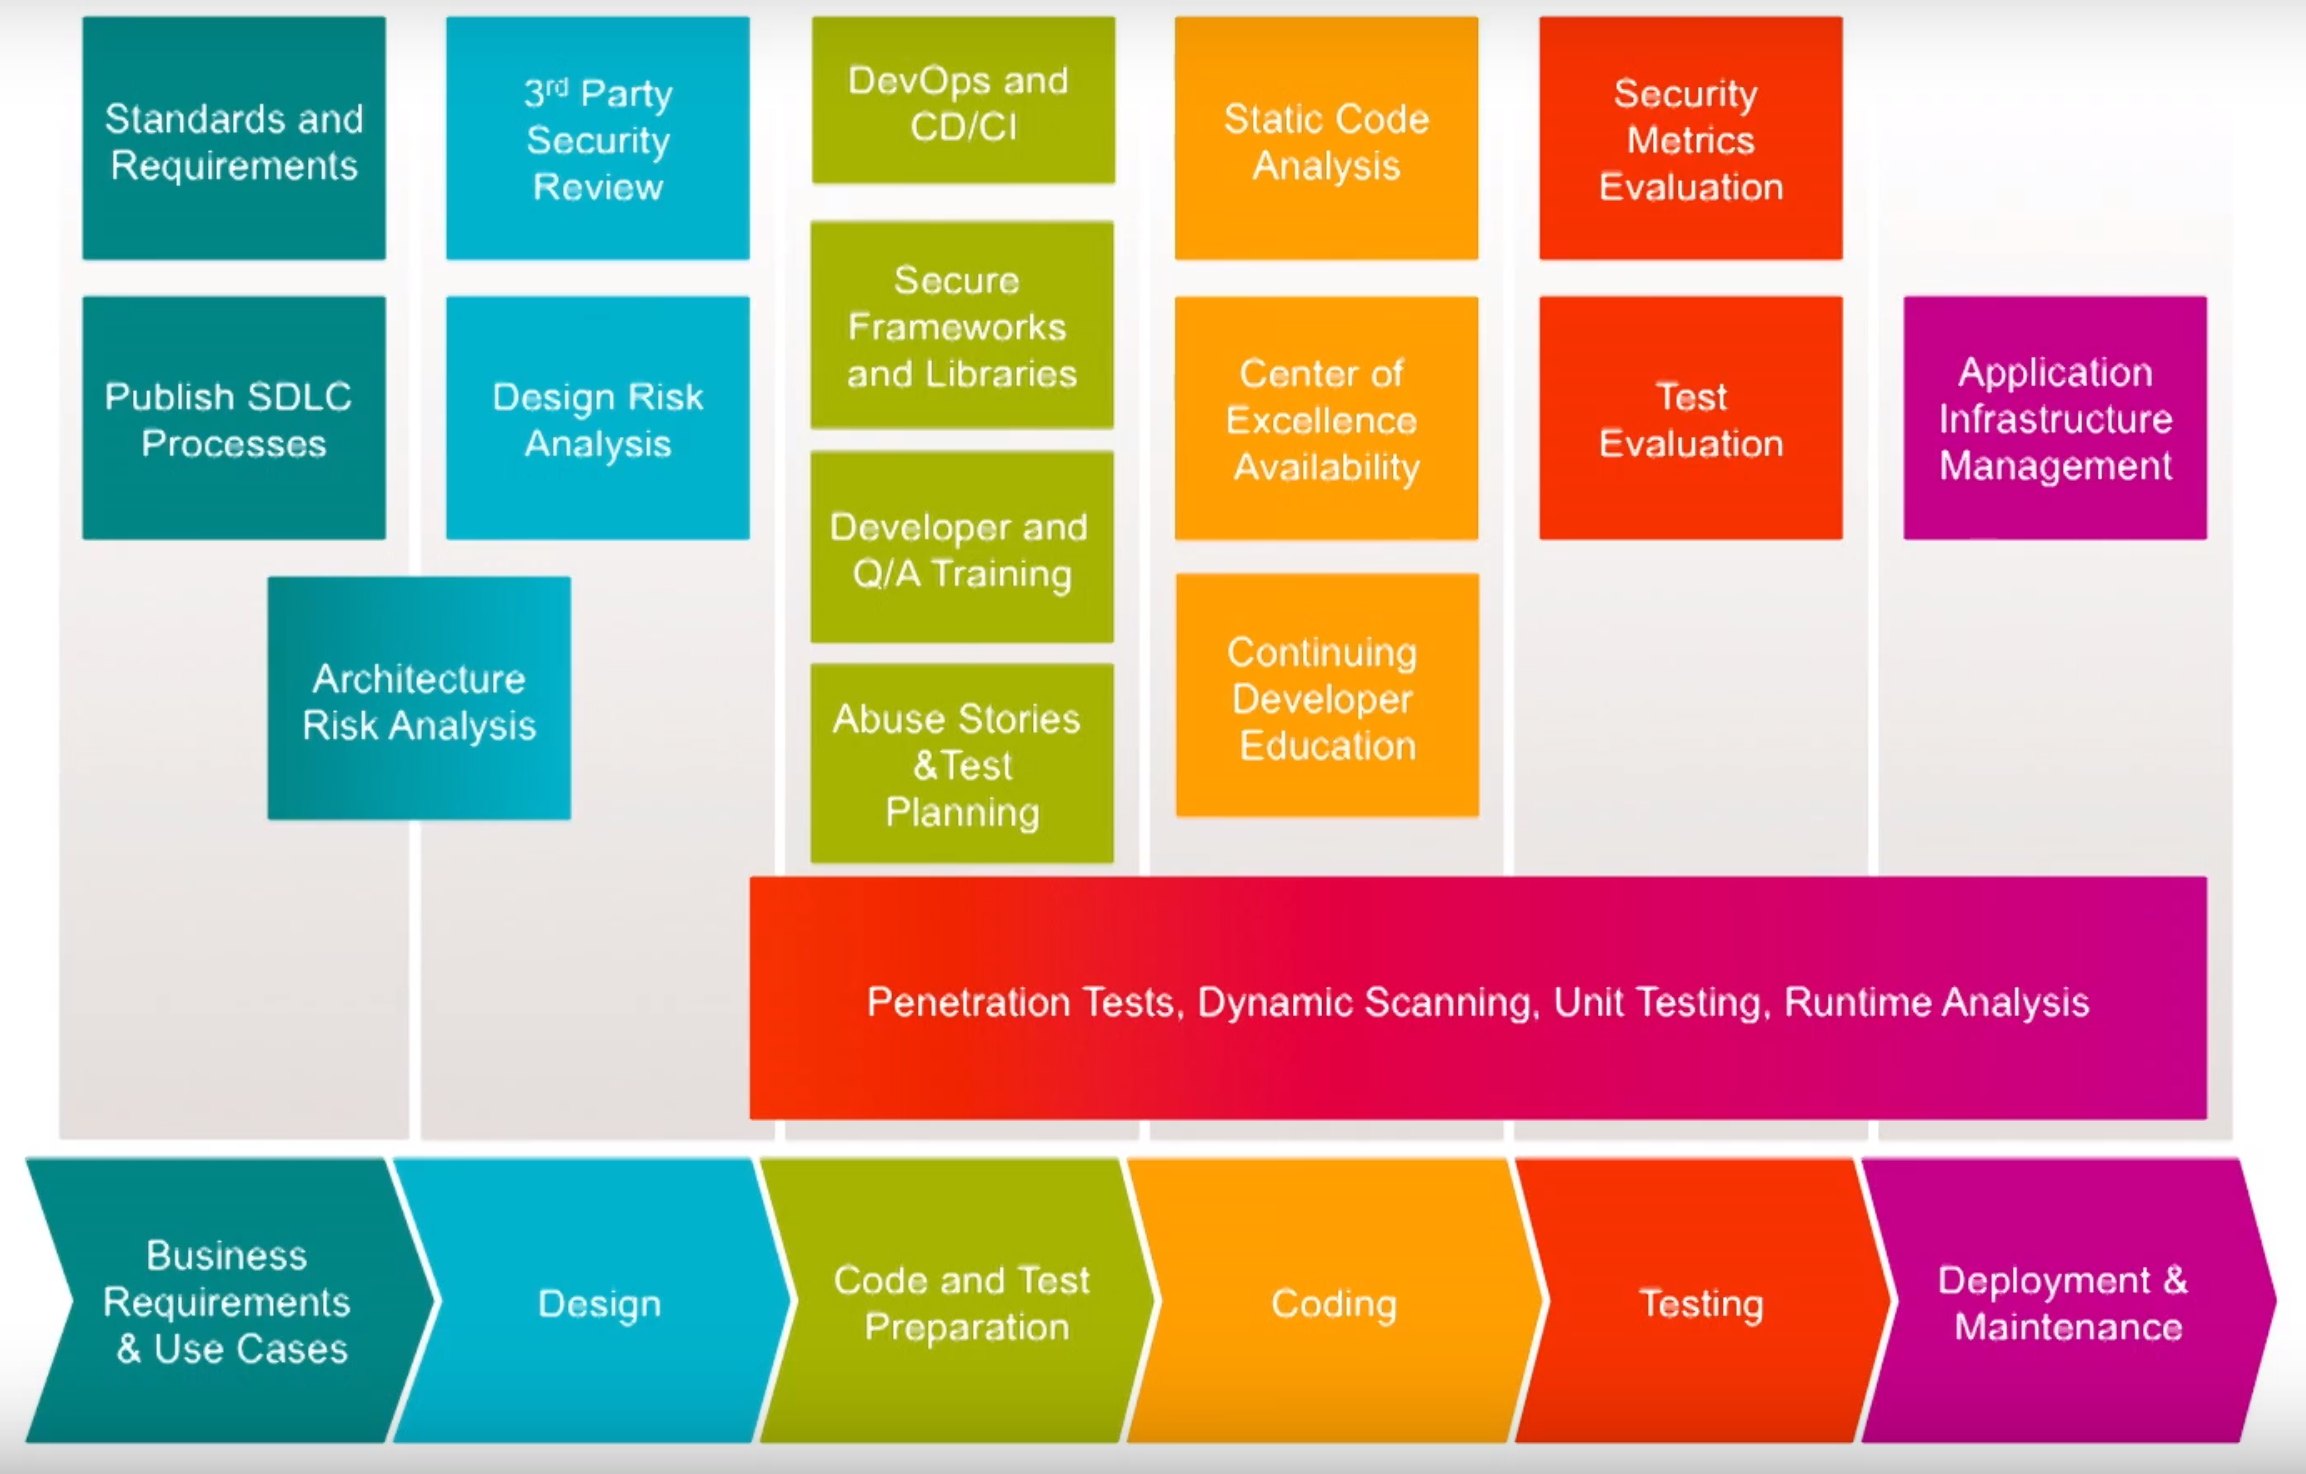
\includegraphics[scale=0.19]{images/JimManicodeSSDLC.png}
    \caption{Security in the SDLC, Jim Manico, dotSecurity 2017.}
    \label{fig:ssdlc}
\end{figure}

Entendiendo que aplicar seguridad en distintas etapas del proceso puede llevar a hallazgos en cada una de ellas, es natural poder separar en categorías cada uno de estos hallazgos. Para ver una representación de cómo sería ver la Figura \ref{fig:ssdlc}.
Si lo que se encuentra corresponde a la etapa de diseño, tienden a ser fallas en las especificaciones y la arquitectura del sistema; vulnerabilidades de implementación son fallas técnicas a bajo nivel en la construcción real del software, y finalmente, en la categoría de vulnerabilidades operacionales  entran las fallas que suceden por deployments y configuración del software en un entorno en particular.

Sin ir más lejos, los costos para solucionar un bug en algunas de estas etapas, tanto para proyectos ágiles o en cascada, empeoran mientras más tarde se encuentran.

A continuación se mencionan algunos hechos relevantes y destacados por su impacto, relacionados a bugs de fallas de seguridad. 
El Mariner 1 de la NASA fue el primer intento de Estados Unidos de enviar una nave espacial a Venus. Poco después de su lanzamiento en 1962, se desvió del rumbo debido a un error de software. Un empleado de la \textbf{NASA} se vio obligado a mandar a la nave a autodestruirse. Se quemaron \$ 18 millones de dólares debido a un guión (-) faltante en el código\cite{TrueCostSoftBugCelerity}.

En febrero del 2018 los servicios web de \textbf{Amazon} no estuvieron disponibles durante 4 horas y afectaron a innumerables sitios. Aunque el costo financiero no está claro, las estimaciones de cuando el sitio de Amazon se cayó en 2016 durante 20 minutos fue de \$ 3.75 millones. El incidente de este verano fue 12 veces más largo e involucró a muchos otros sitios web.

\textbf{AT\&T} actualizó su software para llamadas de larga distancia en enero de 1990. Sin embargo, no se percataron de que el sistema no podría mantenerse al día con la velocidad del nuevo programa. Las llamadas de larga distancia cayeron durante 9 horas. Se perdieron 200,000 reservas de aerolíneas y hubo 75 millones de llamadas telefónicas perdidas. El costo total estimado para AT\&T fue de \$ 60 millones \cite{TrueCostSoftBugCBT}.

El Instituto de Ciencias de Sistemas de \textbf{IBM} ha informado que \textit{el costo de reparar un error después de la publicación del producto fue de cuatro a cinco veces más que uno descubierto durante el diseño, y hasta 100 veces más que uno identificado en la fase de mantenimiento.}


\subsection{Costos en el tiempo}
Phil Crosby, autor que contribuyó a las prácticas de la gestión de la calidad, en su libro \textbf{Quality is free} (La calidad es gratis) explica cuánto cuesta la mala calidad a largo plazo en un proyecto. Simplificadamente se puede interpretar en el gráfico de la Figura \ref{fig:cost of a defect}. El cual intenta demostrar que mientras más temprano, y en etapas más internas se puedan localizar los problemas, más económico será el costo/tiempo de resolverlos, ya que se involucrará menos gente en el proceso.

\begin{figure}[h]
    \centering
    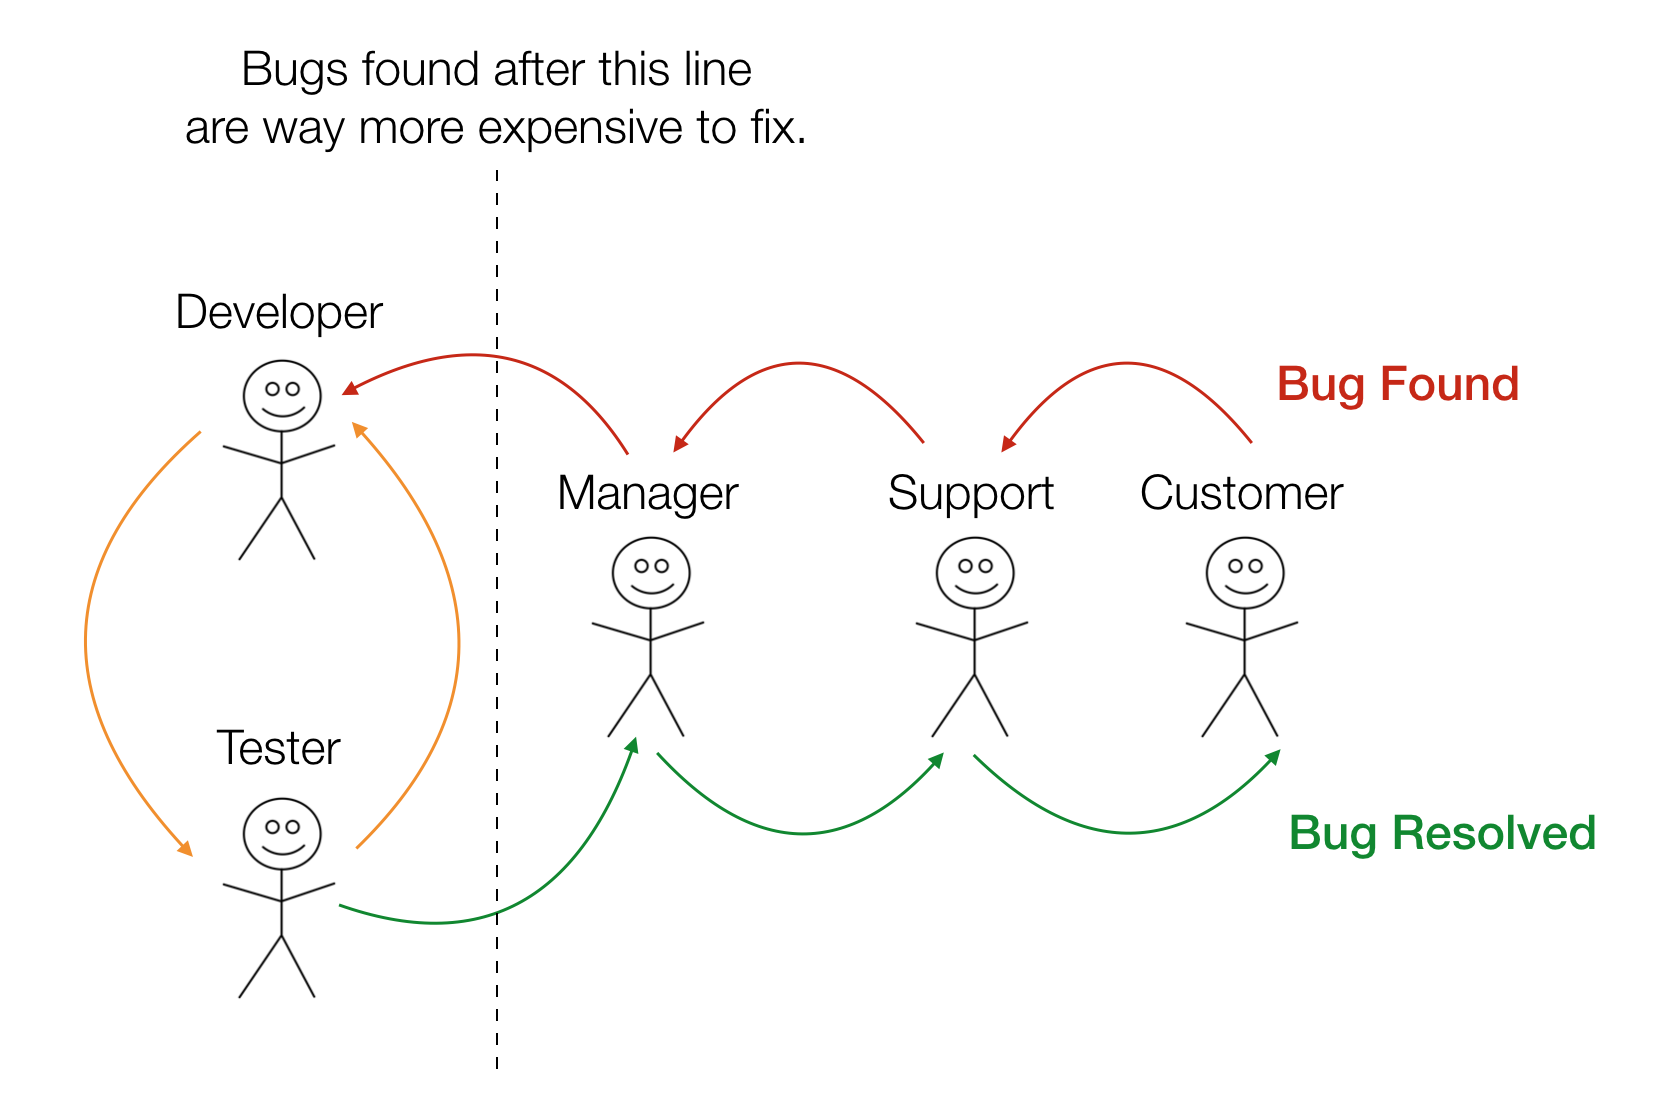
\includegraphics[scale=0.5]{images/the_cost_of_a_defect.png}
    \caption{Cost of a software bug, Emanuil Slavov.}
    \label{fig:cost of a defect}
\end{figure}

Para un ciclo de desarrollo en cascada, según Caper Jones, especialista en metodologías de ingeniería de software, y asociado con el modelo de punto de función de estimación de costos, en su libro Applied Software Measurement: Assuring Productivity and Quality\cite{jones2008applied} el costo para corregir un bug en las distintas etapas se ve descrito por el gráfico de la Figura \ref{fig:applied cost measurement}

\begin{figure}[h]
    \centering
    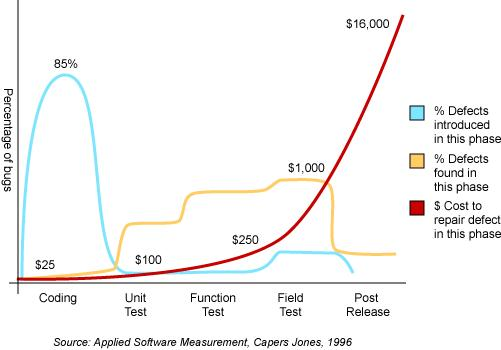
\includegraphics[scale=0.5]{images/AppliedSoftwareMeasurement.png}
    \caption{Applied Software Measurement, Caper Jones, 1996.}
    \label{fig:applied cost measurement}
\end{figure}

Steve McConnell autor de muchos libros de texto de ingeniería de software conocidos, como \textbf{Code Complete}\cite{mcconnell2004code}, \textbf{Rapid Development}\cite{mcconnell1996rapid}, y \textbf{Software Estimation}\cite{mcconnell2006software}, en su primero también realiza un análisis en la dirección de Caper Jones. En la Figura \ref{fig:defect cost increase}, de uno de sus libros se puede observar el costo de detectar un defecto en determinadas etapas.

\begin{figure}[h]
    \centering
    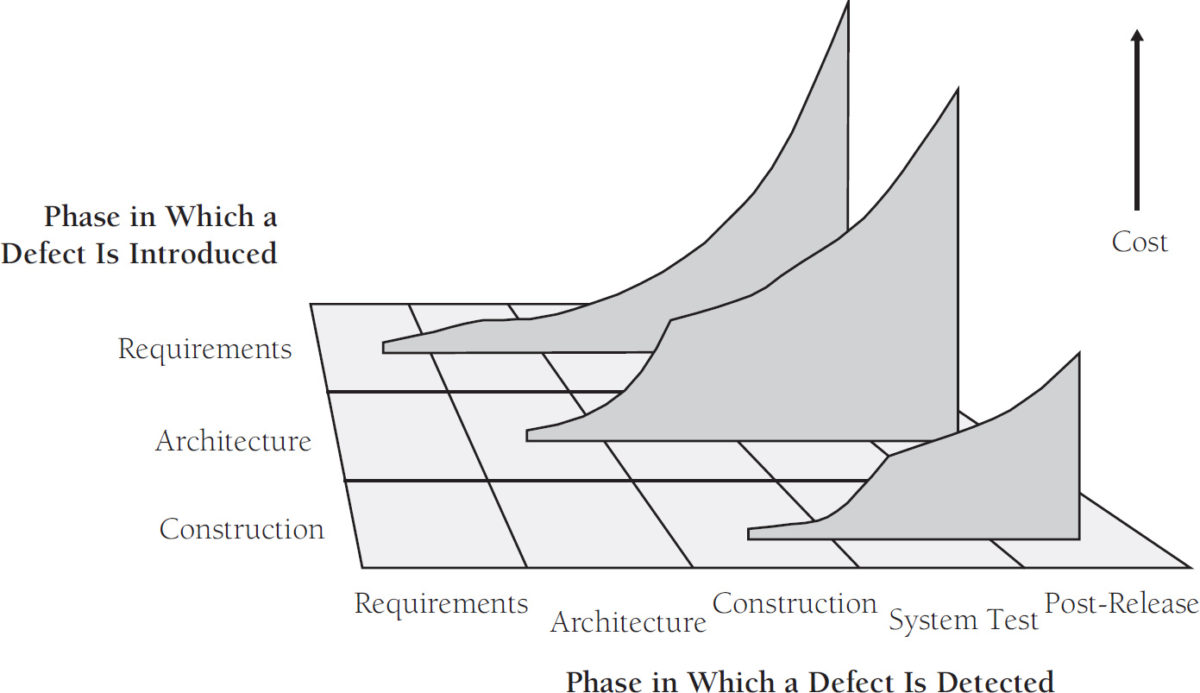
\includegraphics[scale=0.3]{images/DefectCostIncrease2004.jpg}
    \caption{Costo de encontrar defectos por fase, Steve McConnell en Code Complete, 2004.}
    \label{fig:defect cost increase}
\end{figure}

En la Figura \ref{fig:cost-of-change curve} se encuentra una visualización de un artículo sumamente detallado, llamado The Agile Difference for SCM\cite{TheAgileDifference} (La diferencia ágil para la administración de la cadena de suministro), comparando los costos para los distintos modelos: XP, Boehm y Ágil.

\begin{figure}[h]
    \centering
    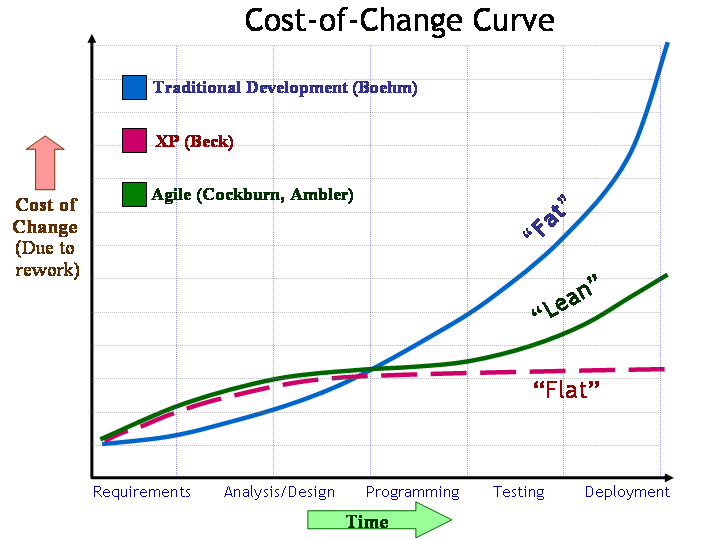
\includegraphics[scale=0.5]{images/TheAgileDifference.png}
    \caption{Curvas del costo de un cambio, CM Crossroads.}
    \label{fig:cost-of-change curve}
\end{figure}

Scott W. Ambler un ingeniero de software, consultor, autor de varios libros centrados en el kit de herramientas de Disciplined Agile Delivery, el proceso Unificado, el desarrollo de software Agile, el Lenguaje de modelado unificado y el desarrollo del Modelo de madurez de capacidades. En su publicación \textbf{Why Agile Software Development Techniques Work: Improved Feedback}\cite{ambler2006agile} (Por qué las técnicas ágiles de desarrollo de software funcionan: Feedback mejorado) se puede observar otro gráfico en relación a los costos con respecto a lo avanzado que se está en el desarrollo del proyecto:

\begin{figure}[h]
    \centering
    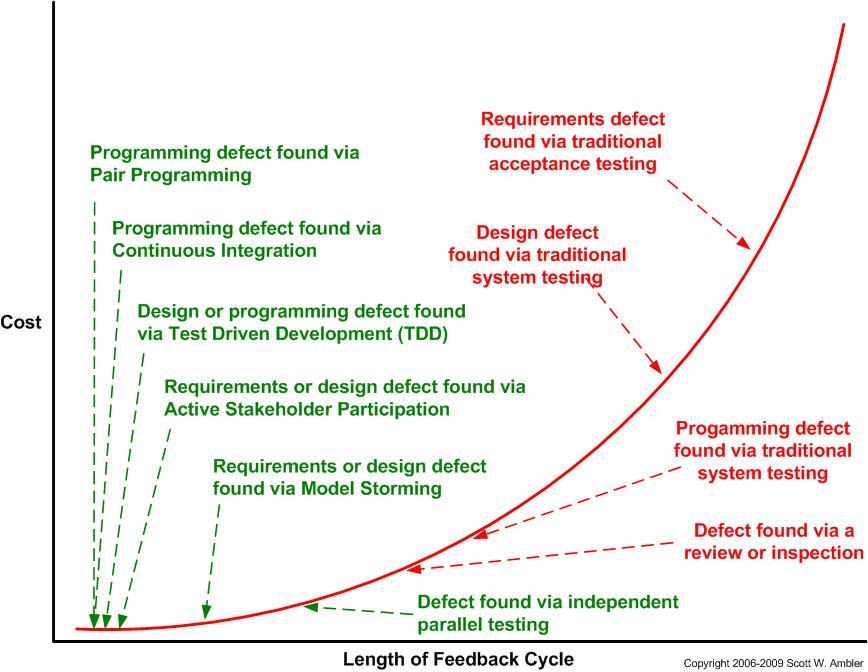
\includegraphics[scale=0.5]{images/ComparingTechniques.jpg}
    \caption{Longitud y costo de un defecto dentro del ciclo de desarrollo, Scott W. Ambler}
    \label{fig:cost-of-change curve}
\end{figure}

A esta altura se puede asumir que el lector tiene una interpretación, al menos visual, respaldada de distintas fuentes con años de trayectoria de lo que cuesta posponer la búsqueda de problemas y solucionarlos en etapas tempranas.

Ahora, hay que entender que estos estudios no contemplan errores de seguridad, ya que tienden a ser superiores, porque si son vulnerabilidades explotables, tienen un impacto directo y dañino, en la empresa y sus consumidores; los impactos directos de reputación también no fueron cuantificados en los estudios anteriores.

Las violaciones a la seguridad cuestan al rededor 600 mil millones de dólares al año globalmente\cite{mcafeecsis}. El 46\% de los incidentes de ciberseguridad del 2017 son debidos a personas internas a la organización\cite{kasperskyHumanFactor}. El 30\% de los profesionales de seguridad esperan un gran y efectivo ataque dentro de los próximos 90 días.\cite{theeconomistCyberChasm}

La mayoría de las fallas en los mecanismos de seguridad están relacionadas a funcionalidad faltante o incorrecta, y la mayoría de las vulnerabilidades están relacionadas a comportamientos adversos no intencionales. 

Michael Felderer, et. al., explican muy bien en su sección de Security Testing\cite{FELDERER20161} en Advances in Computers, 2016:
Las pruebas (funcionales) normalmente se centran en la presencia de algún comportamiento correcto, pero no en la ausencia de un comportamiento adicional, que está implícitamente especificado por requisitos negativos. Las pruebas rutinariamente omiten las acciones ocultas y el resultado son comportamientos peligrosos de efectos secundarios que se envían con un software. La Figura \ref{fig:functionality side-effects} siguiente ilustra esta naturaleza de efectos secundarios de la mayoría de las vulnerabilidades de software que las pruebas de seguridad tienen que enfrentar\cite{FELDERER20161}.

\begin{figure}[h]
    \centering
    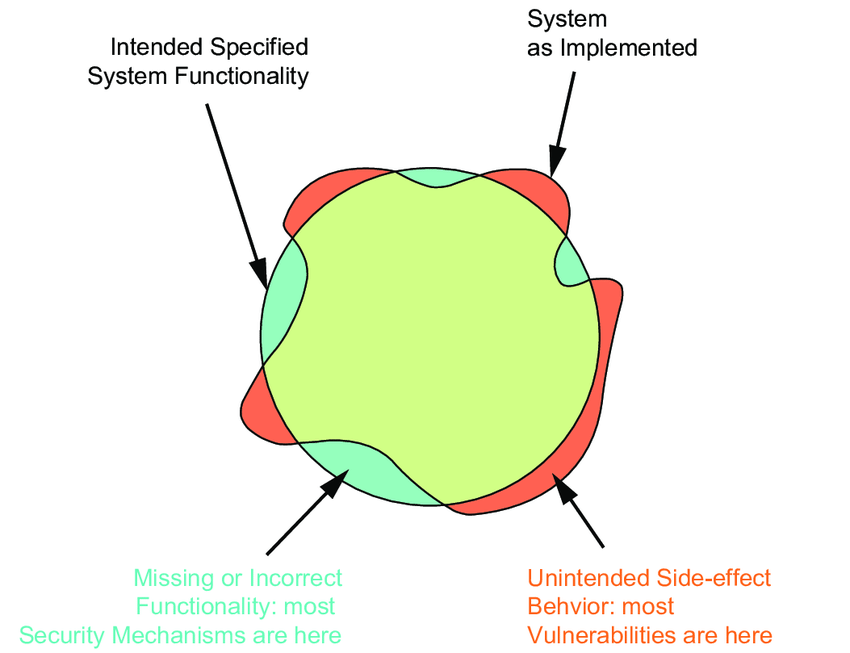
\includegraphics[scale=0.5]{images/functionality.png}
    \caption{Security Testing: A Survey, Michael Felderer.}
    \label{fig:functionality side-effects}
\end{figure}

El círculo representa la funcionalidad prevista de una aplicación, incluidos los mecanismos de seguridad, que generalmente se define mediante la especificación de requisitos. La forma amorfa superpuesta en el círculo representa la funcionalidad real e implementada de la aplicación. En un sistema ideal, la aplicación codificada se superpondría completamente con su especificación, pero en la práctica, este casi nunca es el caso. Las áreas del círculo que la aplicación codificada no cubre representan fallas funcionales típicas (es decir, comportamiento que se implementó incorrectamente y no se ajusta a la especificación), especialmente también en los mecanismos de seguridad. Las áreas que quedan fuera de la región circular representan una funcionalidad no intencionada y potencialmente peligrosa, donde residen la mayoría de las vulnerabilidades de seguridad. La falta de coincidencia entre la especificación y la implementación que se muestra en la figura que conduce a fallas en los mecanismos de seguridad y vulnerabilidades se puede reducir teniendo en cuenta los aspectos de seguridad y especialmente las pruebas de seguridad en una etapa temprana y en todas las fases del ciclo de vida del desarrollo de software.

Dentro de la misma investigación, y basándose de manera abstracta a partir de técnicas de prueba de seguridad concretas mencionadas anteriormente, se clasifican en la siguiente figura de acuerdo con su base de prueba dentro del SSDLC.

\begin{figure}[h]
    \centering
    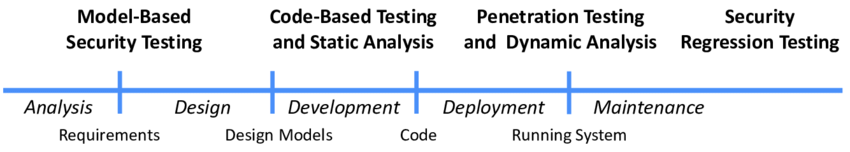
\includegraphics[scale=0.5]{images/TechniquesInTheSSDLC.png}
    \caption{Técnicas de prueba de seguridad en el ciclo de vida de desarrollo de software seguro.}
    \label{fig:ssdlc techniques}
\end{figure}

Las pruebas de \textit{seguridad basadas en modelos} se basan en requisitos y modelos de diseño creados durante la fase de análisis y diseño. Las \textit{pruebas basadas en código y el análisis estático} se basan en el código fuente y el bytecode creado durante el desarrollo. Las \textit{pruebas de penetración y el análisis dinámico} se basan en sistemas en ejecución, ya sea en un entorno de prueba o de producción. Finalmente, las \textit{pruebas de regresión de seguridad} se realizan durante el mantenimiento.


\section{Proceso de revisión de software}
Cuando se tiene que comenzar con el proceso de revisar, desde la perspectiva de seguridad, un software que jamás se ha visto, teniendo una ventana de tiempo generalmente acotada, hay que entender cómo utilizar los recursos y poder cubrir bien las partes que son más relevantes a la seguridad.

Adoptando un proceso pragmático, flexible y basado en resultados se podrá obtener un balance para descubrir fallas de diseño, lógicas, operacionales y de implementación.

Hay dos frases que se destacan mucho de uno de los libros más importantes que he el autor ha tenido la oportunidad de leer en esta investigación, y son \textit{"la revisión de código es un proceso fundamentalmente creativo"}, y \textit{"hacer revisión de código es una habilidad"}. 

Entendiendo esto entonces, la mejor manera de realizarlo es armando una lista de todo lo que probablemente pueda salir mal, y al hacer la revisión tratar de entender al desarrollador pensando en situaciones que no haya podido anticipar. Es una especie de estudio del perfil (profiling) del equipo de desarrollo, y entender que no sólo pueden tener fallas a nivel código sino también conceptuales que en el mismo proyecto pueden traer consecuencias a la forma de encarar otras partes del mismo proyecto, o futuros. Por ejemplo, puede que para un \textit{input} (entrada) de usuario no se estén realizando los chequeos necesarios pero que no tenga ningún impacto real de seguridad; lo que no significa que en otros lugares del mismo proyecto esté aplicado de una forma diferente, pudiendo así explotar finalmente la falla, ya que ha sido conceptual o de diseño.

Tener un proceso es algo realmente valioso más allá de que hay más factores involucrados que simplemente seguir unos pasos. No todos los que realicen el mismo proceso obtendrán los mismos resultados, pero sí probablemente los haga más efectivos. Un proceso le da estructura a la auditoría, permite mantener un nivel de prioridades y ser consistente en el análisis. También de esta manera, junto con documentación permite que los asesoramientos sean algo compatible desde la perspectiva de negocios, lo cual no es algo menor, y es poco común.

El proceso de revisión que se mencionará a continuación, del cual hablan Mark Dowd, John McDonald, y Justin Schuhes, sobre la \textit{identificación y prevención de vulnerabilidades de software}, es abierto, adaptable a los requerimientos de cada equipo para prácticas reales, y está dividido en 4 etapas:
\begin{itemize}
\item \textbf{Pre asesoramiento:} recolección de información inicial y documentación; planeamiento y alcance de la auditoría.
\item \textbf{Revisión:} fase principal del asesoramiento. No está necesariamente estructurada en distintas etapas del ciclo de desarrollo. De hecho, estas etapas son objetivos simultáneos alcanzados por el uso de distintas estrategias. 
\item \textbf{Documentación y análisis:} documentación de procesos, hallazgos, y análisis sobre los mismos para evaluar riesgos y posibles métodos de solución. 
\item \textbf{Reporte y soporte de soluciones:} esta fase es básicamente para darle un seguimiento a quienes van a actuar en base a los hallazgos reportados.
\end{itemize}

\subsection{Pre asesoramiento}
En esta etapa se trata de obtener la mayor cantidad de información posible, porque a partir de ella se va a dictaminar cómo comenzar y qué acercamiento tomar frente a la auditoría.

Hay que definir bien el alcance del proyecto, tal vez sea buscar la vulnerabilidad más impactante del proyecto como también obtener la mayor cobertura del código posible sin la necesidad de comprobar que sean explotables o no las fallas encontradas. Esto no sólo va a depender de quién esté realizando la auditoría sino también del propósito de la misma.

Como forma tangible del software en cuestión se puede proveer tanto el código, como el binario, o ambos. La combinación del código y el binario, o un setup en el cual desde el código se pueda llegar al binario, son lo que hacen una revisión más eficiente (no siempre se puede llegar del código a un ejecutable). Sin un binario, ni la posibilidad de compilar, generalmente se realizan análisis estáticos, y en las potenciales fallas encontradas resultan difíciles de comprobar su real explotación. Sin el código fuente, no hay otra alternativa que realizar análisis en ejecución e ingeniería inversa (analizar el código assembler del ejecutable).

Existen otras alternativas, como poseer el binario con información adicional de debugging (símbolos por ejemplo) que facilita la ingeniería inversa, usualmente entregado por empresas con software propietario que quieren simplificar la revisión. Y el caso más extremo, usualmente más utilizado al realizar auditorías web, es cuando no se entrega código ni binario, en donde sólo se realizan técnicas externas como \textit{black box} y \textit{fuzzing} (*).

\textit{Fuzzing} es una forma de descubrir errores en el software al proporcionar entradas aleatorias a programas para encontrar casos de prueba que causan un \textit{crash} (detenimiento abrupto). Aplicando técnicas de \textit{fuzzing} a programas, se puede obtener una vista rápida de la solidez general y ayudar a encontrar y corregir errores críticos. Es una técnica de \textit{black box}, que no requiere acceso al código fuente, pero aún puede usarse contra el software para el que se posee dicho fuente, ya que posiblemente encuentre los errores más rápido, evitando la necesidad de revisar muchas líneas de código. Una vez que se detecta un bloqueo, si se tiene el código fuente, debería ser mucho más fácil de solucionar o explotar una vulnerabilidad.

En el caso de proyectos open source, como el que se verá en el caso de estudio, es donde se posee el mejor escenario. Para estos, siempre es mejor realizar una revisión manual de código, y como tal se debe comenzar con un \textit{threat model} (modelado de amenazas) o al menos entrevistas a los desarrolladores para tener un entendimiento de la arquitectura de la aplicación, su superficie de ataque, así como también las técnicas de implementación.

\subsection{Revisión}
La tendencia principal a la hora de comenzar es generalmente seguir un modelo en cascada, lo cual no siempre es el mejor camino o el único, como ya se ha hablado anteriormente, más si se está hablando en términos de ser tiempo-eficiente identificando vulnerabilidades en alto como bajo nivel.
Parecerá obvio pero un auditor se encuentra más preparado para juzgar la seguridad del diseño o implementación, al finalizar la auditoría que al principio. Esto es, hablando en términos de entenderlo de manera abstracta.

No siempre se puede comenzar por el diseño o haciendo un \textit{threat model}, a veces la documentación no existe, está incompleta, vieja; los desarrolladores pueden también no estar disponibles.

El método para realizar la revisión es un simple proceso iterativo. Particularmente se planea qué estrategia utilizar, y dependiendo de ella la selección de técnicas u objetivos. Después se ejecuta la estrategia seleccionada tomando notas, y de vez en cuando reflexionar sobre el manejo del tiempo, para no obsesionarse particularmente con algo que demande demasiado. Finalmente entender qué es lo que se ha aprendido y ver cómo utilizarlo, repitiendo estos pasos hasta el final de la auditoría.

Hay tres maneras generalizadas para realizar la evaluación: \textit{top-down}, \textit{bottom-up}, e híbrida; las primeras dos son análogas a los tipos de descomposición de componentes en el diseño de software, y la última una combinación de ambas, alternando, dependiendo cuanta información se tenga del contexto dado.

En la etapa de planeamiento se elige qué tipo de estrategia se utilizará, en las próximas secciones se detalla brevemente las recomendadas por estos autores. La selección, la preparación para la misma y demás detalles se realizan dependiendo si se trabaja en equipo, con metas/objetivos específicos, y preparación de la toma de notas/documentación que se va a acontecer. También se pone sobre la mesa hacer un chequeo general del estado de la evaluación, re-evaluar si la estrategia seleccionada está funcionando, y conducir \textit{peer-reviews} para tener más objetividad.

\subsection{Documentación y análisis}
En esta etapa, luego de que el trabajo difícil ha terminado, se documentan o formalizan las notas que se tomaron con los hallazgos. 

Principalmente se puede describir el tipo de amenaza, el componente afectado, el módulo (línea de código) donde se encontró, a qué clase de vulnerabilidad pertenece, una descripción con el resultado y el contexto para reproducirla. Finalmente el riesgo o impacto que produce.

Se decidió no entrar en detalles en cómo es cada una de las categorías ya que son bastante explicativas por sí solas, y depende de la dedicación que se le quiera abocar a cada una, tanto como agregar mas o utilizar menos.

\subsection{Reporte y soporte de soluciones}
Finalizar una auditoría no consta solamente de entregar lo hallado de manera organizada. Se cumple un rol muy importante a la hora de entregar, ya que sin alternativas, soluciones o sin mantener un contacto para ayudar a remediar los problemas reportados nos estaría faltando una parte muy importante de nuestro trabajo.

Dependiendo del tipo de auditoría que se esté realizando, esta etapa puede implicar situaciones más complejas. En caso de una investigación independiente, en la circunstancia de haber encontrado vulnerabilidades explotables que pueden perjudicar a otros usuarios, se debe iniciar un disclosure (divulgación) responsable. Generalmente se desarrollan exploits (programa particularmente diseñado y/o utilizado para abusar vulnerabilidades en un determinado sistema) antes de contactar al proveedor de ese software/servicio, y una vez contactado, en el caso de respuesta, se otorgan 30-90 días para solucionar el problema antes de hacerlo público.

\begin{notesBox}
    \textbf{Recorrer el código}
    Al autor le parece importante dejar expresado brevemente la importancia que tiene saber recorrer un código, porque es lo que se va a estar haciendo la mayor parte del tiempo, y dependiendo de la manera en la que se haga va a condicionar la velocidad y dificultad de su progreso.

    Generalmente, lo que es más efectivo es revisar funciones de manera aislada, y hacer seguimiento al flujo sólo cuando es absolutamente necesario.

\end{notesBox}

\section{Estrategias de auditoría de código}
Las estrategias se pueden resumir a las siguientes tres categorías:

\subsection{Compresión de código (CC):}
Estas estrategias analizan el código directamente para descubrir vulnerabilidades y mejorar el entendimiento de la aplicación.

En esta categoría se encuentran las siguientes metodologías: seguimiento de \textit{inputs} maliciosos, analizar un módulo, analizar un algoritmo, analizar una clase u objeto y seguimiento de cosas de interés por usar \textit{black box}.

Exceptuando por el seguimiento a los resultados encontrados realizando \textit{black box}, todas ellas son difíciles y lentas, pero todas las comprensiones de los impactos hallados serán altísimas.

\subsection{Puntos candidatos (CP):}
Se requieren dos pasos: Primero crear una lista de problemas potenciales mediante un proceso o mecanismo y luego examinar el código en busca de ellos.

En la lista mencionada se encuentran las siguientes estrategias: herramientas automatizadas de análisis del código; puntos candidatos de enfoque general, léxicos simples, binarios simples, generados por \textit{black box}, y específicos de aplicación. Estas estrategias se destacan por ser rápidas, fáciles de realizar pero la comprensión de su impacto suele ser bajo.

\subsection{Generalización de diseño (DG):}
Estas técnicas, son más flexibles, intencionadas para analizar potenciales problemas de medianos a alto nivel en la lógica y el diseño.

En ella se encuentran las siguientes sub-estrategias: modelado del sistema, testeo de hipótesis, deduciendo propósito y funcionalidad, y chequeo de conformidad de diseño.

Son de nivel moderado a difícil, velocidad media, pero con altísima comprensión del impacto.

\section{Tácticas de auditoría de código}
En esta sección se presenta un análisis de las tácticas más relevantes de auditoría de código, este análisis está basado mayormente en el capítulo \textit{6.4.9} del libro \textit{The Art of Vulnerability Assessment} previamente mencionado.

\subsection{Análisis de flujo interno}
Muchos caminos poseen secciones similares de código, por lo tanto analizar los que sean relevantes no es tanto trabajo como parece, además de que es totalmente posible leer varios caminos en simultáneo.

Se pueden ignorar las fallas de chequeo de errores ya que no son relevantes a la seguridad, pero hay que tener extremo cuidado cuando se descartan partes con este criterio, ya que es bastante común descuidarse en dos áreas en particular: ramas de chequeos de errores, las rutas que el código sigue cuando los chequeos de validación resultan en error; y rutas de código patológicas, funciones con pequeñas rutas que no resultan con una terminación abrupta de su funcionalidad (\textit{crash}).

\subsection{Análisis de subsistema y dependencias}
No sólo es necesario revisar los módulos que interactúan directamente con los datos ingresados por los usuarios, también es importante entender los subsistemas y las dependencias que estos mismos utilizan. Algunos ejemplos son las maneras que utilizan para hacer manejos de memoria, APIs de sistema, subsistemas que manejan guardado de datos, parsers de cadenas de caracteres, manejos de buffers de datos, etcétera.


\subsection{Releer código}
Releyendo el código es una de las únicas maneras para lograr terminar de entenderlo, si se quiere se puede interpretar como un proceso iterativo, en donde las primeras pasadas pueden utilizarse para concentrarse en vulnerabilidades más evidentes.


\subsection{Chequeando con lápiz y papel}
Si hay partes del código a las cuales se les puede hacer un seguimiento con diversos tipos de datos de entrada, se puede trabajar sobre lápiz y papel como se enseña en la facultad, para ver si responde acorde. A muchos les sorprendería los resultados que se obtienen con este simple, pero efectivo mecanismo.


\subsection{Casos de test}
Realizar casos de test es algo muy útil, y no solo se pueden realizar llamando al binario desde otro programa (wrapper) con diversas entradas, sino que se pueden realizar casos de test como haría uno mismo si estuviera desarrollando el software. También, en la experiencia del autor, ha partido de casos de test provistos por el proyecto y se ha pivotado hacia una perspectiva más de seguridad para encontrar cosas relevantes.


\section{Herramientas para la auditoría}
Existen una gran cantidad de herramientas para facilitar el proceso. Herramientas como navegadores de código\cite[]{CodeCompassLink}\cite[]{SourceInsightLink}\cite[]{UnderstandLink}\cite[]{SourceTrailLink}, analizadores de código estático\cite{clangLink}\cite[]{coverityLink}\cite[]{cppcheckLink}\cite[]{codesonnarLink}\cite[]{inferLink}\cite[]{awesomeStaticList}, analizadores del software en ejecución/debuggers \cite[]{radare2Link}\cite[]{gdbLink}\cite[]{lldbLink}\cite[]{windbgLink}\cite[]{ollydbgLink}, navegadores de binarios/disassemblers\cite[]{binnaviLink}\cite[]{capstoneLink}\cite[]{idaproLink}\cite[]{binaryninjaLink}\cite[]{ghidraLink}, fuzzers\cite[]{aflLink}\cite[]{radamsaLink}\cite[]{grammarinatorLink}\cite[]{honggfuzzLink}\cite[]{awesomeFuzzlist}, y más.

El autor no entrará en detalle, ya que describir todos carece de sentido, y que no todos sirven para todos los contextos, además hablará con detalle más adelante respecto a los que fueron utilizados en el caso de estudio.

\section{Auditoría de compiladores}
El foco del caso de estudio está dado en un software que su vez es un compilador.

\subsection{Arquitectura}
Los compiladores cumplen un rol muy importante en el desarrollo de software. Su principal función es convertir un código fuente en un lenguaje adecuado para su manipulación por humanos en un código ejecutable, cercano a una computadora real o virtual, correspondiente a una o varias arquitecturas. 

Los compiladores se encuentran organizados por etapas sucesivas, apreciadas en la Figura 2.9 a continuación, y entre cada una de ellas se manipulan datos de naturalezas específicas. En general, los compiladores pueden verse como traductores, donde cada traducción requiere procesos de análisis y síntesis.

\begin{figure}[h]
    \centering
    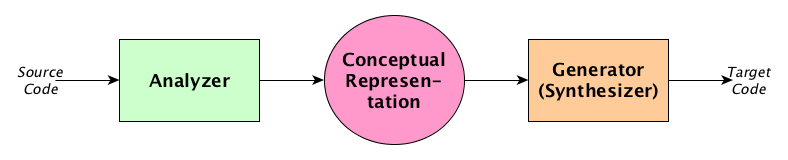
\includegraphics[scale=0.5]{images/analsyn.png}
    \caption{Arquitectura. Ray Toal, Loyola Marymount University.}
    \label{fig:compiler architecture}
\end{figure}


El desarrollo de los compiladores sigue un esquema conocido como “Teoría de Compiladores” el cual tiene su raíz junto con el nacimiento de la computación misma y más precisamente con los primeros lenguajes de programación de alto nivel. Esta teoría ha sido consolidada por varios autores\cite{aho1990compiladores}\cite{srikant2002compiler}\cite{slonneger1995formal}\cite{aho1990compiladores}\cite{meduna2007elements}\cite{appel2004modern}\cite{morgan1998building}\cite{terry1997compilers}\cite{grune2012modern}\cite{tremblay1985theory}\cite{lee1974anatomy}\cite{cooper2011engineering}\cite{gupta2010compiler}\cite{reps2007program}\cite{mak2011writing}\cite{midkiff2012automatic}\cite{seidl2012compiler}\cite{srikant2002compiler}\cite{su2011principles}\cite{mogensen2017introduction} y con el surgimiento de nuevos lenguajes de programación\cite{dasnois2011haxe}\cite{mccurdy2015haxe}\cite{klabnik2018rust}\cite{matzinger2019hands}\cite{sharma2019mastering}\cite{donovan2015go}\cite{summerfield2012programming}\cite{guney2018hands}\cite{skeen2018kotlin}\cite{adelekan2018kotlin}\cite{yousefkotlin} contínuamente está siendo puesta a prueba sin que esto haya significado modificaciones esenciales en el esquema. El caso del lenguaje Rust, de la fundación Mozilla\cite{mozillarustdoc} cuyo compilador se encuentra documentado\cite{mozillarustcdoc} en los términos de la Teoría de Compiladores, es una prueba fehaciente que las nuevas construcciones sintácticas y semánticas sobre seguridad de memoria, closures y paralelización pueden ser soportadas sin problemas por dicha teoría.

Ambas etapas están compuestas de fases internas que serán descritas en las siguientes secciones.

\subsubsection{Componentes}
A continuación brevemente se describen los componentes para un compilador que genera lenguaje ensamblador. En casos en los que los compiladores están diseñados para lenguajes de más alto nivel, o hacia máquinas virtuales, algunas de las etapas descritas son obviadas.

\begin{figure}[h]
    \centering
    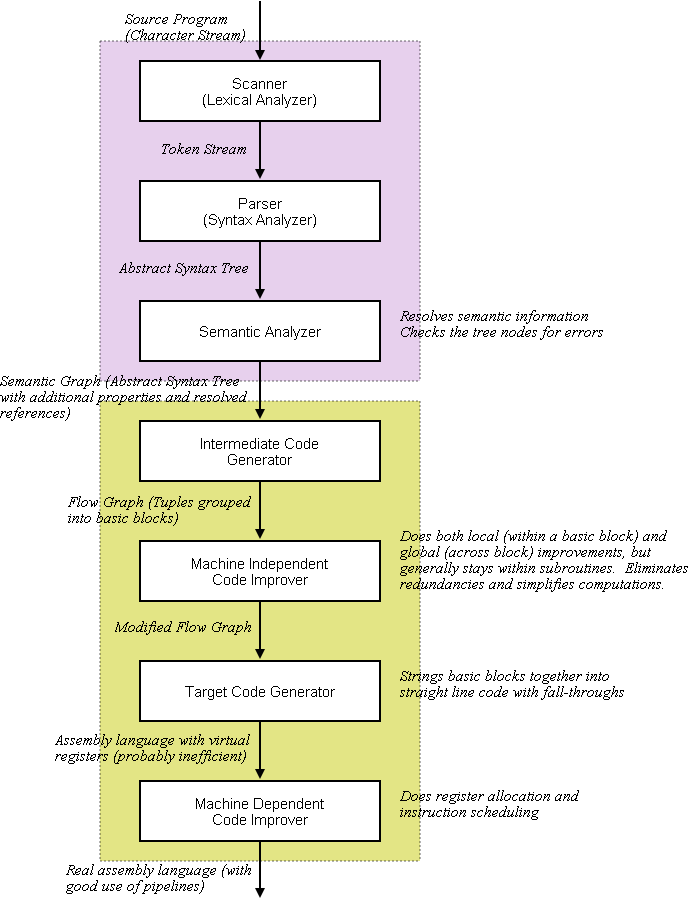
\includegraphics[scale=0.3]{images/compilerphases.png}
    \caption{Componentes de un compilador. Ray Toal, Loyola Marymount University.}
    \label{fig:compiler phases}
\end{figure}


\subsubsection{Análisis léxico (Scanner)}
El scanner convierte el flujo de caracteres correspondiente al código fuente del programa en un flujo de tokens.
Desde el código del recuadro \ref{lst:example} se puede llegar al conjunto de tokens mostrado en la Figura \ref{fig:tokens}.


\begin{lstlisting}[language=c, label={lst:example}, caption={Código de ejemplo}, captionpos={b}, frame={shadowbox}]
#define ZERO 0
unsigned  gcd (
    unsigned int x,// Algoritmo Euclideo
        unsigned y) {
            while ( /* hello */ x> ZERO) {
                unsigned temp=x;
                x=y%x;y  = temp;
            }
        return y;
}
\end{lstlisting}

\begin{figure}[h]
    \centering
    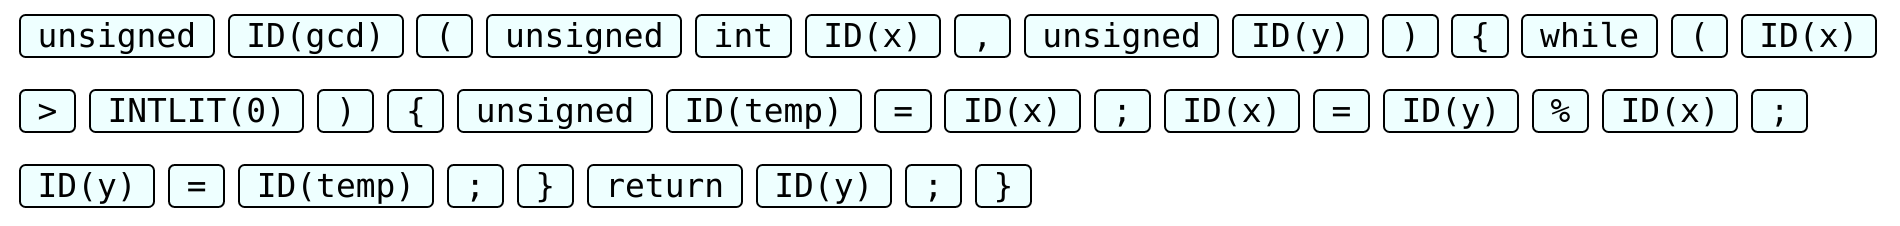
\includegraphics[scale=0.2]{images/tokens.png}
    \caption{Conjunto de tokens. Ray Toal, Loyola Marymount University.}
    \label{fig:tokens}
\end{figure}

Los escáneres se ocupan de cuestiones tales como:
\begin{itemize}
    \item Sensibilidad de mayúsculas y minúsculas (o insensibilidad)
    \item Si los espacios en blanco son significativos o no
    \item Si las nuevas líneas son significativas
    \item Si los comentarios pueden anidarse
\end{itemize}

Los errores que pueden ocurrir durante el escaneo, llamados errores léxicos, incluyen:
\begin{itemize}
    \item Encontrar caracteres que no están en el alfabeto de idioma
    \item Demasiados caracteres en una palabra o línea
    \item Un caracter no cerrado o cadena literal
    \item Un final de archivo dentro de un comentario
\end{itemize}

\subsubsection{Análisis sintáctico (Parsing)}

\begin{figure}[h]
    \centering
    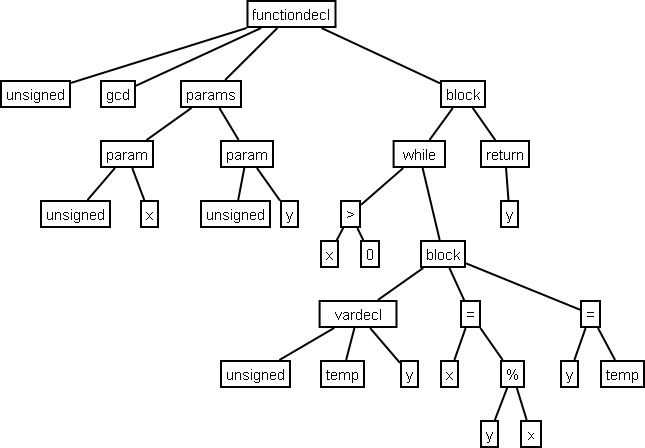
\includegraphics[scale=0.3]{images/gcdast1.png}
    \caption{Árbol sintáctico abstracto. Ray Toal, Loyola Marymount University.}
    \label{fig:ast}
\end{figure}

El árbol también puede ser guardado en forma de un string (cadena de caracteres) como es mostrado en el recuadro \ref{lst:string}

\begin{lstlisting}[label={lst:ast}, caption={AST}, captionpos={b}, frame={shadowbox}]
(fundecl unsigned gcd
  (params (param unsigned x) (param unsigned y))
  (block
    (while
      (> x 0)
      (block (vardecl unsigned temp y) (= x (% y x)) (= y temp)))
    (return y)))
\end{lstlisting}

Técnicamente, cada nodo en el AST se almacena como un objeto con campos con nombre, muchos de cuyos valores son nodos en el árbol. Hay que tener en cuenta que en esta etapa de la compilación, el árbol es definitivamente solo un árbol como se ve en la Figura \ref{fig:ast objects}. No hay ciclos.

\begin{figure}[h]
    \centering
    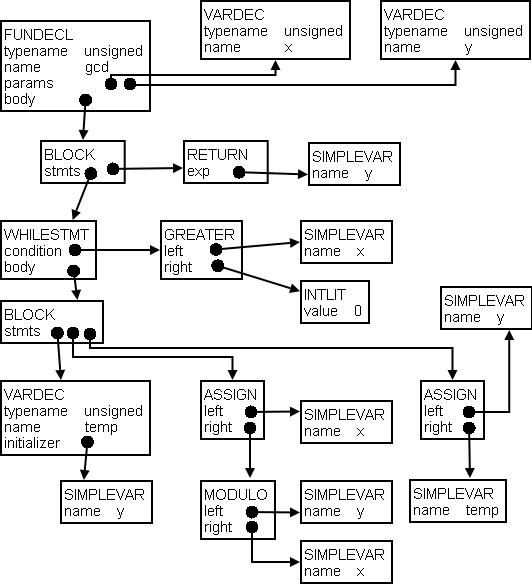
\includegraphics[scale=0.3]{images/gcdast2.png}
    \caption{Vista de objetos del AST. Ray Toal, Loyola Marymount University.}
    \label{fig:ast objects}
\end{figure}

Los errores que pueden ocurrir durante el análisis, llamados errores de sintaxis incluyen cosas como las siguientes, en C:

\begin{itemize}
    \item \texttt{42 = x * 3}
    \item \texttt{i = /5}
    \item \texttt{j = 4 * (6 - x;}
\end{itemize}


\subsubsection{Análisis semántico}
Durante el análisis semántico se deben verificar las reglas de legalidad y, al hacerlo, atar las piezas del árbol de sintaxis (resolviendo las referencias de los identificadores, insertando operaciones de conversión para coerciones implícitas, etc.) para formar un gráfico semántico.

Continuando con el ejemplo anterior, el AST se puede apreciar como en la Figura \ref{fig:ast semantic}.

\begin{figure}[h]
    \centering
    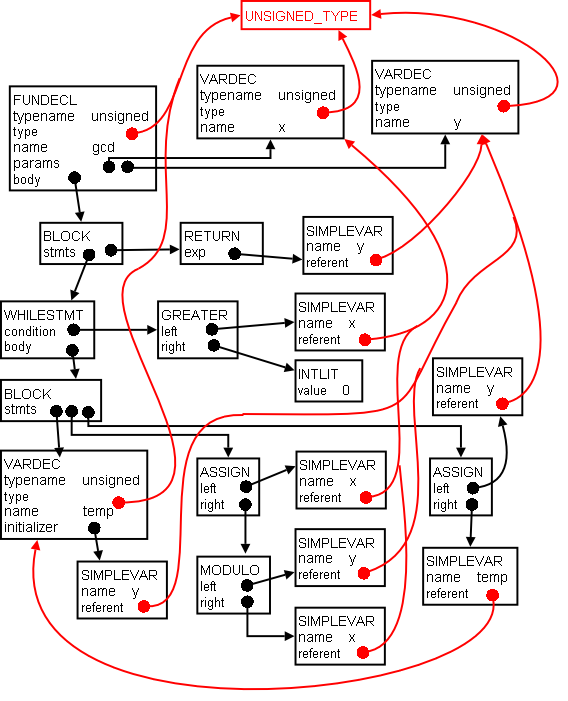
\includegraphics[scale=0.3]{images/gcdsemgraph.png}
    \caption{AST con análisis semántico. Ray Toal, Loyola Marymount University.}
    \label{fig:ast semantic}
\end{figure}

Obviamente, el conjunto de reglas permitidas es diferente para cada idioma. Los ejemplos de que se pueden ver en un lenguaje similar a Java incluyen:
\begin{itemize}
    \item Múltiples declaraciones de una variable dentro de un ámbito.
    \item Referencia a una variable antes de su declaración.
    \item Referencia a un identificador que no tiene declaración.
    \item Violar las reglas de acceso (público, privado, protegido, ...).
    \item Demasiados argumentos en una llamada de método.
    \item No hay suficientes argumentos en una llamada de método.
    \item Tipo de desajustes (hay toneladas de estos).
\end{itemize}

\subsubsection{Generación de código intermedia}
El generador de código intermedio produce un gráfico de flujo formado por \textit{tuplas} agrupadas en bloques básicos. Para el ejemplo anterior, se ve en la Figura \ref{fig:flowchart intermediate}.

\begin{figure}[h]
    \centering
    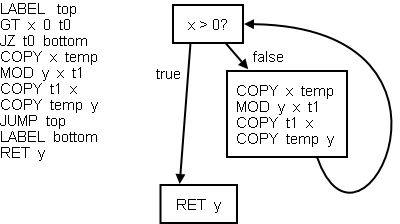
\includegraphics[scale=0.3]{images/gcdflowgraph.png}
    \caption{Gráfico de flujo intermedio. Ray Toal, Loyola Marymount University.}
    \label{fig:flowchart intermediate}
\end{figure}

\subsubsection{Mejoras de código independientes de la arquitectura}
La mejora de código que se realiza en el gráfico semántico o en el código intermedio se denomina optimización de código independiente de la arquitectura. En la práctica hay una gran cantidad de optimizaciones conocidas\cite{srikant2018compiler}\cite{emmanuel2017newtrends} (mejoras), pero ninguna realmente se aplica a nuestro ejemplo de ejecución.

\subsubsection{Generación de código}
No se pretende que el lector interprete el assembler, sino que se aprecie que mediante una optimización la lógica del programa se mantiene y su salida es más pequeña.

La generación de código produce el código de destino real, o algo cercano. Esto es lo que se obtiene al ensamblar con gcc 6.3 orientado a x86-64, sin ninguna optimización.

\begin{lstlisting}[language={[x86masm]Assembler}, label={lst:assembler simple}, caption={Ejemplo assembler sin mejora}, captionpos={b}, frame={shadowbox}]
gcd(unsigned int, unsigned int):
    pushq   %rbp
    movq    %rsp, %rbp
    movl    %edi, -20(%rbp)
    movl    %esi, -24(%rbp)
.L3:
    cmpl    $0, -20(%rbp)
    je      .L2
    movl    -20(%rbp), %eax
    movl    %eax, -4(%rbp)
    movl    -24(%rbp), %eax
    movl    $0, %edx
    divl    -20(%rbp)
    movl    %edx, -20(%rbp)
    movl    -4(%rbp), %eax
    movl    %eax, -24(%rbp)
    jmp     .L3
.L2:
    movl    -24(%rbp), %eax
    popq    %rbp
    ret
\end{lstlisting}


\subsection{Mejora de código dependiente de la arquitectura}

Por lo general, la fase final en la compilación es limpiar y mejorar el código objetivo. Para el ejemplo anterior, se obtiene lo siguiente al configurar el nivel de optimización en -O3:
\begin{lstlisting}[language={[x86masm]Assembler}, label={lst:assembler improved}, caption={Ejemplo assembler con mejora}, captionpos={b}, frame={shadowbox}]

gcd(unsigned int, unsigned int):

        testl   %edi, %edi
        movl    %esi, %eax
        jne     .L3
        jmp     .L7
.L5:
        movl    %edx, %edi
.L3:
        xorl    %edx, %edx
        divl    %edi
        movl    %edi, %eax
        testl   %edx, %edx
        jne     .L5
.L1:
        movl    %edi, %eax
        Ret
.L7:
        movl    %esi, %edi
        jmp     .L1
\end{lstlisting}


\section{¿Por qué compiladores?}
Siempre se pone el foco y la responsabilidad del lado del lenguaje en el que los desarrolladores programan, pero más allá de testear, se está totalmente confiando en que el compilador que se utiliza no posea fallas de seguridad, y que como mínimo no vaya a introducir nuevas en el código desarrollado.


La seguridad informática es un desafío bastante amplio impuesto sobre el sistema. Sólo se necesita una parte que sea insegura y todo el sistema se vuelve inseguro. Sería muy dificultoso para un compilador corregir automáticamente código inseguro, ya que para ello, debería tener en su concepción una gran cantidad de aspectos pragmáticos aún no conocidos en el momento de su construcción. Pero más allá de lo anterior, el compilador está colocado perfectamente en una posición que permite ayudar a un programador o ingeniero de software a escribir sistemas seguros. La razón es porque el compilador es el único programa que tiene la posibilidad de mirar (casi) todas las líneas de un software. Obviamente lenguajes compilados como C/C++ pasan por un compilador, pero lenguajes semi-interpretados como Java también tienen un compilador para generar su bytecode e incluso código assembler es típicamente pre-procesado por el compilador. Las únicas excepciones podrían ser los lenguajes puramente interpretados, con algunos otras casos muy particulares\cite{secenhancedcompilers}, aunque la interpretación puede verse como una suerte de compilación en línea, compilación bajo demanda o compilación JIT (\textit{Just in Time})\cite{bolc2012design}\cite{mak2011writing}.

\textit{¿Hasta dónde debería uno confiar que una declaración en un programa está libre de Caballos de Troya? Tal vez es más importante confiar en las personas que desarrollaron el software directamente.}

Lo describe claramente Ken Thompson, desde 1984 en su artículo \textbf{Reflections on trusting trust} (reflecciones en confiar en la confianza):
\begin{displayquote}
    \textit{"La moral es obvia. No podés confiar en un código que no creaste en su totalidad. (Especialmente el código de compañías que emplean a personas como yo). Ninguna verificación o escrutinio a nivel de fuente te protegerá de usar código no confiable. Al demostrar la posibilidad de este tipo de ataque, elegí el compilador de C. Podría haber elegido cualquier programa de manejo de software, como un ensamblador, un cargador o incluso un microcódigo de hardware. A medida que el nivel del programa disminuye, estos errores serán cada vez más difíciles de detectar. Un bug de microcódigo bien instalado será casi imposible de detectar."}
    \newline{\null\hfill -- Ken Thompson}
\end{displayquote}

El "ataque" del cual habla está separado en dos etapas, y consta de cómo hipotéticamente modifica un compilador para generar backdoors (puertas traseras). En la primera etapa, el código en C contiene código visiblemente obvio para modificar la lógica dado un patrón determinado, de un programa de acceso, y como bien dice:
\textit{Tal descarado código no pasaría desapercibido por mucho tiempo. Incluso la lectura más casual del código fuente del compilador de C levantaría sospechas.}

En la segunda etapa es donde la modificación de un compilador con fines maliciosos se pone interesante. En adición a agregar código al compilador de C para corromper un programa en particular también agrega código al compilador para corromperse a sí mismo. Es decir, que si se compilara con ese compilador maligno otro compilador en base a un código limpio, se agregaría la lógica necesaria al nuevo compilador para que cada vez que procese un software de acceso le inserte un \textit{backdoor}.

No necesariamente tiene que ser con intenciones malignas, así como hay errores de seguridad en la mayoría de los programas, un compilador no está exento a esto, y las mismas fallas podrían generar comportamientos inesperados en la compilación.


\subsection{Optimizaciones y comportamiento inesperado}
Investigadores del laboratorio de Ciencias de la computación e inteligencia artificial del MIT publicaron un paper (\textit{Towards Optimization-Safe Systems: Analyzing the Impact of Undefined Behavior}) analizando el problema optimización de código inestable, el cual es código que el compilador quita porque incluye comportamiento indefinido. Dicho código es el que puede comportarse de maneras inesperadas, como dividir por cero, una desreferencia de puntero nulo y \textit{buffer overflows} (rebalse de búferes).

A diferencia de otro código, los desarrolladores de compiladores son libres de decidir cómo lidiar con este tipo de comportamientos. En algunos casos eligen eliminar ese código completamente, lo cual puede llevar a vulnerabilidades si el código en cuestión posee chequeos de seguridad.

Estos investigadores estudiaron una docena de compiladores C/C++ más comúnmente utilizados para observar cómo lidian con código indefinido. Encontraron que, con el tiempo, los compiladores están poniéndose más agresivos en cómo lidian con ese código, usualmente sólo quitándolo, incluso por defecto o en pequeños niveles de optimización. Ya que C/C++ es bastante liberal respecto a permitir comportamiento indefinido, es más susceptible a errores y amenazas de seguridad como resultado de código inestable.

Tanto es el hecho que existe una categoría de seguridad específicamente para estos casos, llamada \textit{optimización insegura de compilación}. A continuación un ejemplo.\cite{insecureoptOWASP}

\begin{lstlisting}[language={c}, label={lst:vulnerable code}, caption={Código vulnerable}, captionpos={b}, frame={shadowbox}]
void GetData(char *MFAddr) {
    char pwd[64];
    if (GetPasswordFromUser(pwd, sizeof(pwd))) 
     if (ConnectToMainframe(MFAddr, pwd)) {
             // Interaction with mainframe
        }
      }
      memset(pwd, 0, sizeof(pwd));
}
\end{lstlisting}

El código en el ejemplo del cuadro \ref{lst:vulnerable code} se comportaría correctamente si se ejecutara de manera literal, pero si el código se compila utilizando la opción general de optimización, como las de los compiladores de C++ Microsoft Visual C ++ ® .NET o GCC 3.x, la llamada a memset() se eliminará como un almacenamiento inactivo porque el búfer \textit{pwd} no se usa después de que su valor se sobrescribe. Debido a que el búfer pwd contiene un valor sensible, la aplicación puede ser vulnerable a un ataque si los datos se quedan en la memoria. Si los atacantes pueden acceder a la región correcta de la memoria, pueden usar la contraseña recuperada para obtener el control del sistema.\cite{wikiseicmuedu}
 
Otro ejemplo más impactante que terminó afectando a muchos sistemas Linux/GNU, fue un error introducido en el kernel debido a una optimización.
Si bien los detalles técnicos sobre esto son un poco complejos, en general, lo que sucede puede explicarse fácilmente. El código vulnerable se encuentra en la implementación de una librería. Básicamente, lo que sucede aquí es que el desarrollador inicializó una variable (\textbf{sk} en el fragmento de código a continuación) a un cierto valor que puede ser \textit{NULL}. El desarrollador verificó correctamente el valor de esta nueva variable par de líneas más tarde y, si es 0 (\textit{NULL}), simplemente devuelve un error. El código se ve así:\cite{iscsansedukernelvuln}

\begin{lstlisting}[language={c}, label={lst:kernel vuln}, caption={Código vulnerable 2}, captionpos={b}, frame={shadowbox}]
struct sock *sk = tun->sk;  // initialize sk with tun->sk
...
if (!tun)
    return POLLERR;  // if tun is NULL return error
\end{lstlisting}

Este código se ve perfectamente bien, y lo es, al menos hasta que el compilador toma esto en sus manos. Mientras optimiza el código, verá que la variable ya ha sido asignada y eliminará el bloque \textit{if} (la comprobación si \textit{tun} es NULL) completamente del código compilado resultante. En otras palabras, el compilador introducirá la vulnerabilidad al código binario, que no existía en el código fuente. Esto hará que el kernel intente leer / escribir datos desde la dirección de memoria \textit{0x00000000}, que el atacante puede \textit{mapear} a la zona de usuario, controlando el flujo de ejecución. 

\textbf{Vulnerabilidades en intérpretes}

Los intérpretes no son el foco de discusión en esta investigación, pero el contenido aplica de igualmente manera a ellos también.

Todas las vulnerabilidades alguna vez reportadas tienen asignado un identificador único llamado CVE (Common Vulnerability Enumeration). En el sitio oficial de la lista se puede encontrar que intérpretes como Ruby\cite{rubyvulns}, Python\cite{pythonvulns} y PHP\cite{phpvulns} poseen 13, 45 y 599 vulnerabilidades reportadas hasta el momento de esta redacción.


\section{Tecnologías blockchain}
En esta sección se enumeran tecnologías cuya estructura principal es del tipo blockchain, con las que se trabajó en esta tesis y forman parte de las principales razones por la que fue impulsada esta investigación, dada la popularidad que han obtenido en los últimos años.


\subsection{Bitcoin}
La idea de tener una moneda digital no es nueva. Antes de las \textit{cryptocurrencies} (criptomonedas), existieron muchos intentos de crear una. El principal desafío que la mayoría encontraba era solucionar el problema de \textit{double spend} (doble gasto). Un bien digital tiene que de alguna manera ser utilizado sólo una vez para prevenir que se copie y efectivamente falsifique.\cite{briefhistorycryptoledger}

Diez años antes de las \textit{cryptocurrencies}, el concepto había sido introducido por un ingeniero en computación llamado Wei Dai. En 1998, publicó un paper donde discutió una propuesta llamada \textit{B-money}. Discutió la idea de una moneda digital, que podía ser enviada junto con un grupo de pseudónimos irrastreables. Ese mismo año, otro intento bajo el nombre \textit{Bit Gold} fue escrito por Nick Szabo. Bit Gold incluyó la posibilidad de crear una moneda digital descentralizada. La idea de Szabo fue motivada por las ineficiencias que se encuentran hoy en día en el sistema financiero tradicional (FIAT), como requerir metales para construir monedas, y para reducir la cantidad de confianza que hay que tener para realizar transacciones. Si bien ambos proyectos nunca fueron oficialmente ejecutados, fueron parte de la inspiración de \textit{Bitcoin}\cite{narayanan2016bitcoin}.

En el 2008 Satoshi Nakamoto publicó un artículo (\textit{white paper}) llamado \textit{Bitcoin: A Peer-to-Peer Electronic Cash System}, describiendo la funcionalidad de la red blockchain de Bitcoin: \textit{una red sin permiso tolerante a fallos bizantinos} (resistencia de un sistema informático tolerante a faltas) \textit{criptográficamente segura}.

\begin{displayquote}
    \textit{"Mucha gente descarta automáticamente las e-currency como una causa perdida por todas las compañías que fallaron hacerlo desde 1990. Espero que sea obvio que lo que las llevó a la perdición fue su naturaleza de tener un sistema central controlado. Creo que esta es la primera vez que estamos intentando un sistema descentralizado, no basado en la confianza."}
    \newline{\null\hfill -- Satoshi Nakamoto.}
\end{displayquote}

\subsection{Estructura blockchain}
La blockchain es un libro de registro distribuido punto a punto, seguro, y se utiliza para registrar transacciones. El contenido del registro solo se puede actualizar agregando otro bloque vinculado al anterior. También se puede ver como una plataforma donde las personas pueden realizar transacciones de todo tipo sin la necesidad de un árbitro central o de confianza.

\textit{La base de datos creada se comparte entre los participantes de la red de manera transparente, por lo que todos pueden acceder a su contenidos. La gestión de la base de datos se realiza de forma autónoma utilizando redes punto a punto y un servidor de timestamping, es decir que permite demostrar que una serie de datos han existido y no han sido alterados desde un instante específico en el tiempo. Cada bloque en una blockchain está organizado de tal manera que hace referencia al contenido del bloque anterior.}\cite{101blockchains}

\textit{Los bloques que forman una blockchain contienen lotes de transacciones validadas por los participantes en una red. Cada bloque viene con un hash criptográfico de un bloque anterior en la cadena.}\cite{101blockchains}

\begin{notesBox}
    Bitcoin y Blockchain no son sinónimos. Blockchain es la estructura que Bitcoin posee como base para impulsar sus aplicaciones.
\end{notesBox}


\subsection{Smart Contracts}
Un smart contract es un código de computadora corriendo sobre una blockchain que posee un conjunto de reglas bajo las cuales las partes de ese contrato acceden para interactuar uno con el otro. Si-y-cuando esas reglas se cumplan, el acuerdo es automáticamente impuesto. El código del smart contract facilita, verifica, y hace cumplir la negociación o performance de un acuerdo o transacción. Es la forma más simple de automatización descentralizada.

Es un mecanismo que envuelve bienes digitales de dos o más partes, donde algunas o todas las partes depositan bienes en el contrato y los bienes son automáticamente redistribuidos entre esas partes dependiendo de una fórmula basada en determinados datos, que no son conocidos al momento de la iniciación del contrato. 

El término se presta a confusiones porque un smart contract no es inteligente, ni debería ser confundido con un contrato legal:
\begin{itemize}
    \item Un smart contract es tan inteligente como las personas que lo programaron con la información que tenían disponible en ese momento.
    \item Mientras que tienen el potencial de poder ser contratos legales no deben confundirse con contratos legales aceptados por las cortes y la ley. Sin embargo, probablemente se vaya a ver una fusión de estos dos en el futuro.
\end{itemize}

Si bien la descripción anterior es acertada, y una definición que se puede observar en muchas fuentes, el autor cree que es demasiada específica. Un smart contract es algo más abstracto.

Entonces, se puede resaltar lo más importante de la siguiente manera: son auto verificables, auto ejecutables y resistentes a la manipulación; pueden transformar responsabilidades legales en procesos automatizados, garantizar un gran grado de seguridad, reducen la dependencia de intermediarios confiables y poseen costos de transacción bajos. 


\subsection{Ethereum}
En el 2013 un jóven llamado Vitalik Buterin\cite{miethereumvitalik}, co-fundador de la Bitcoin Magazine propuso \textbf{Ethereum} en un paper llamado \textit{‘Ethereum: A Next-Generation Smart Contract and Decentralized Application Platform’}. Preocupado por las limitaciones de Bitcoin, comenzó a trabajar en lo que él pensaba que sería una blockchain maleable que pueda realizar varias funciones además de ser una red punto a punto. Ethereum\cite{101blockchainseth} nació como una nueva blockchain pública con funcionalidades adicionales, en comparación con Bitcoin.

\begin{displayquote}
\textit{"Bitcoin es excelente como dinero digital, pero su lenguaje de scripting es demasiado débil para que se puedan construir aplicaciones avanzadas de forma seria."}
\newline{\null\hfill -- Vitalik Buterin}
\end{displayquote}

Lanzado oficialmente en 2015, Ethereum ha evolucionado hasta convertirse en una de las aplicaciones más grandes de la tecnología de blockchain, dada su capacidad para respaldar los \textit{smart contracts} utilizados para desarrollar aplicaciones descentralizadas. La plataforma ha logrado reunir una comunidad activa de desarrolladores que la han visto convertirse en un verdadero ecosistema.

Procesa la mayor cantidad de transacciones diarias gracias a su capacidad para soportar contratos inteligentes y aplicaciones descentralizadas. Su capitalización de mercado también se ha incrementado significativamente en el espacio de las criptomonedas.

En la Figura \ref{fig:blockchain history} se muestra una cronología para repasar visualmente el proceso.

\begin{figure}[h]
    \centering
    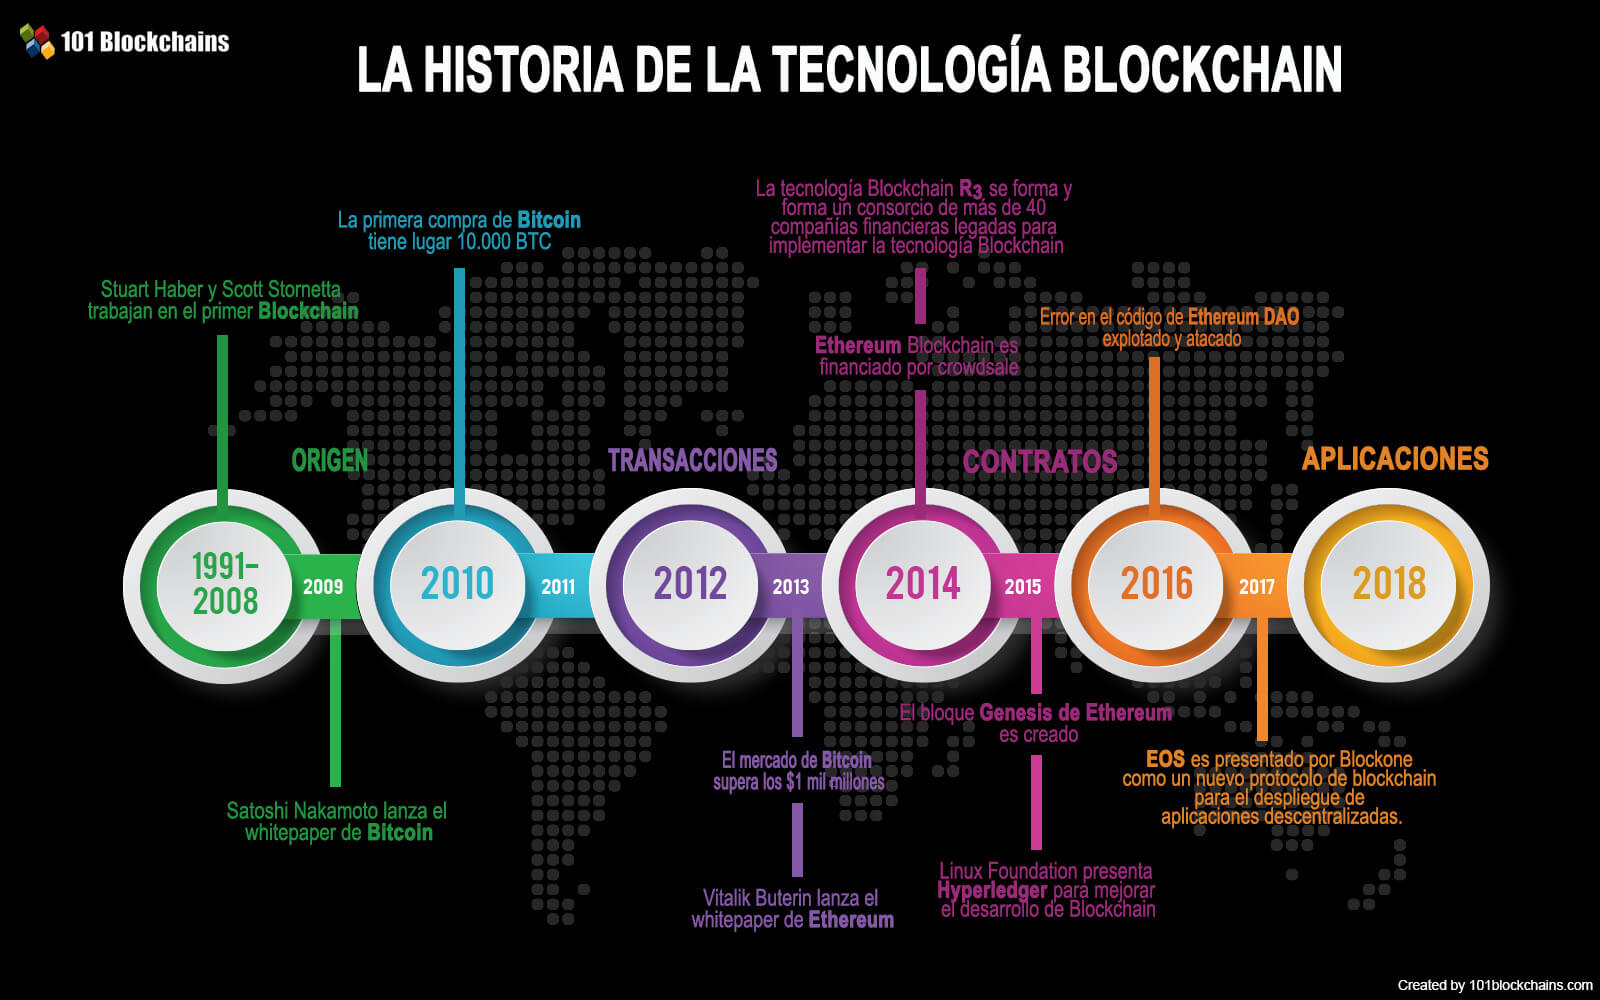
\includegraphics[scale=0.3]{images/historiablockchain.jpg}
    \caption{ Cronología de tecnologías blockchain por 101blockchains.}
    \label{fig:blockchain history}
\end{figure}

\subsection{Ethereum Virtual Machine}
La Ethereum Virtual Machine (\textbf{EVM}) es el contexto en el cual los smart contracts de la red de Ethereum viven y se ejecutan. Posee un stack de registros de 256 bits, diseñada para correr el código exactamente como fue desarrollado. Es el mecanismo de consenso fundamental para Ethereum. La definición formal de la EVM está especificada en el Ethereum Yellow Paper.

\begin{figure}[h]
    \centering
    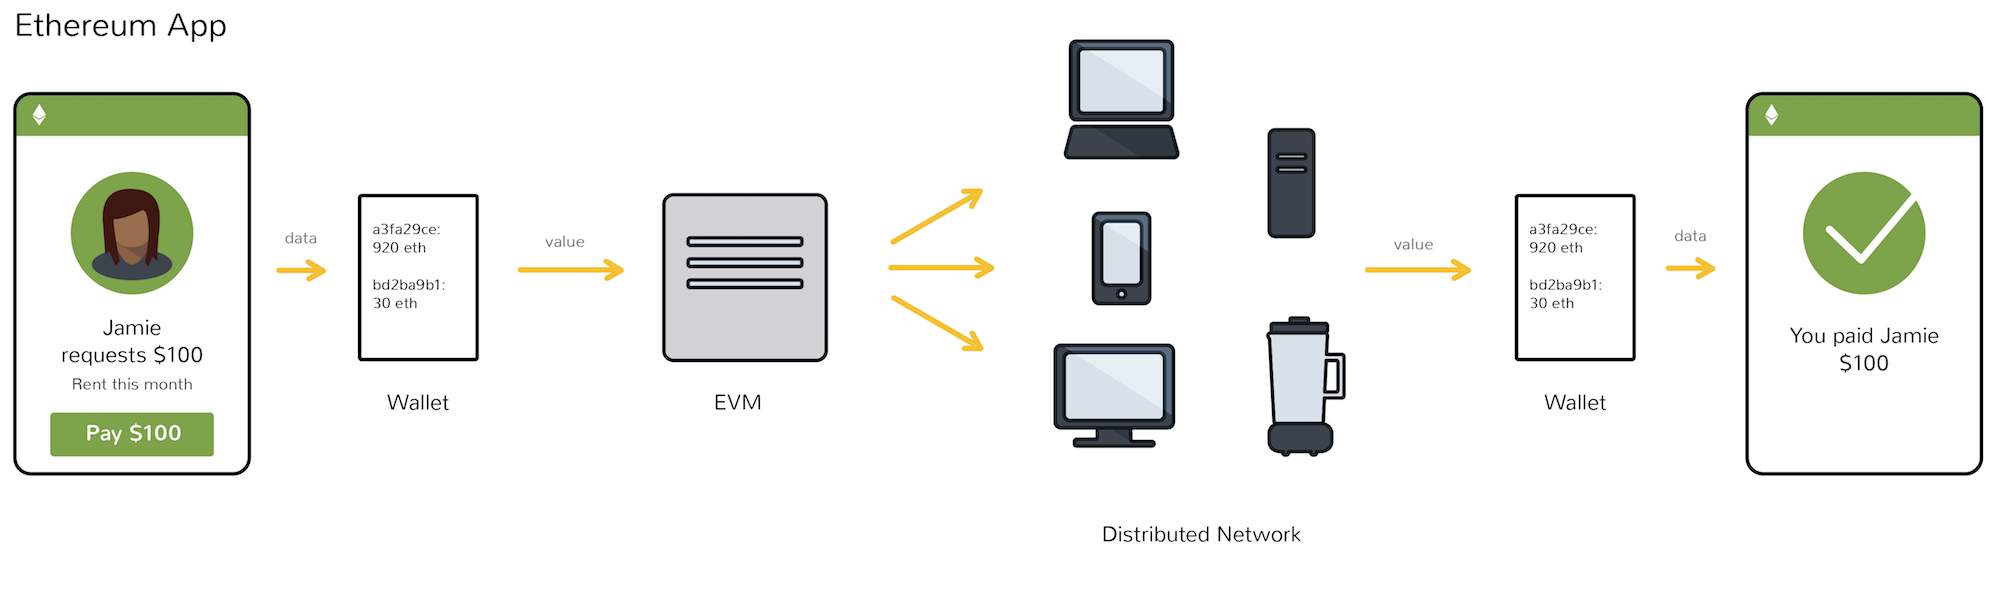
\includegraphics[scale=0.5]{images/ethflowapp.png}
    \caption{Diagrama de despliege, por Coindesk.}
    \label{fig:ethereum app}
\end{figure}

\subsection{¿Cómo es Ethereum diferente a Bitcoin?}
Si bien hay varias similitudes entre Ethereum y Bitcoin, también hay diferencias significativas:
\begin{enumerate}
    \item Bitcoin opera sólo como cryptocurrency, mientras que Ethereum ofrece diversos métodos de interacción, incluyendo cryptocurrency (Ether), smart contracts y la Ethereum Virtual Machine.
    \item Están basados en distintos protocolos de seguridad: Ethereum eventualmente utilizará un sistema \textit{proof of stake} (PoS) en contraposición al sistema \textit{proof of work} (PoW) utilizado por Bitcoin, aunque en este momento utilizan el mismo hasta que el cambio suceda. \textit{Explicar las diferencias y alcances de PoS vs PoW escapa del contexto de la investigación.}
    \item El tiempo promedio de generación de un bloque en Ethereum es de 12 segundos contra 10 minutos de Bitcoin. Esto se traduce a más confirmaciones de bloque, lo que permite a los mineros de Ethereum a completar más bloques y recibir más Ethers.
    \item Ethereum usa un sistema de cuentas en donde los valores en Wei (mínima unidad de representación de un Ether, \verb|1x10^18|) son debitados de una cuenta hacia otra, al contrario del sistema de UTXO (\textit{Unspent Transaction Output}) de Bitcoin, que es más análogo a gastar dinero y recibir cambio. Ver Figura \ref{fig:ethereum state transaction}.
    \item Ethereum posee una máquina virtual que permite escribir smart contracts con un lenguaje bytecode \textit{turing completo}.
    \item La moneda de Bitcoin se representa mediante la sigla BTC, y la de Ethereum mediante ETH.
\end{enumerate}

\begin{figure}[h]
    \centering
    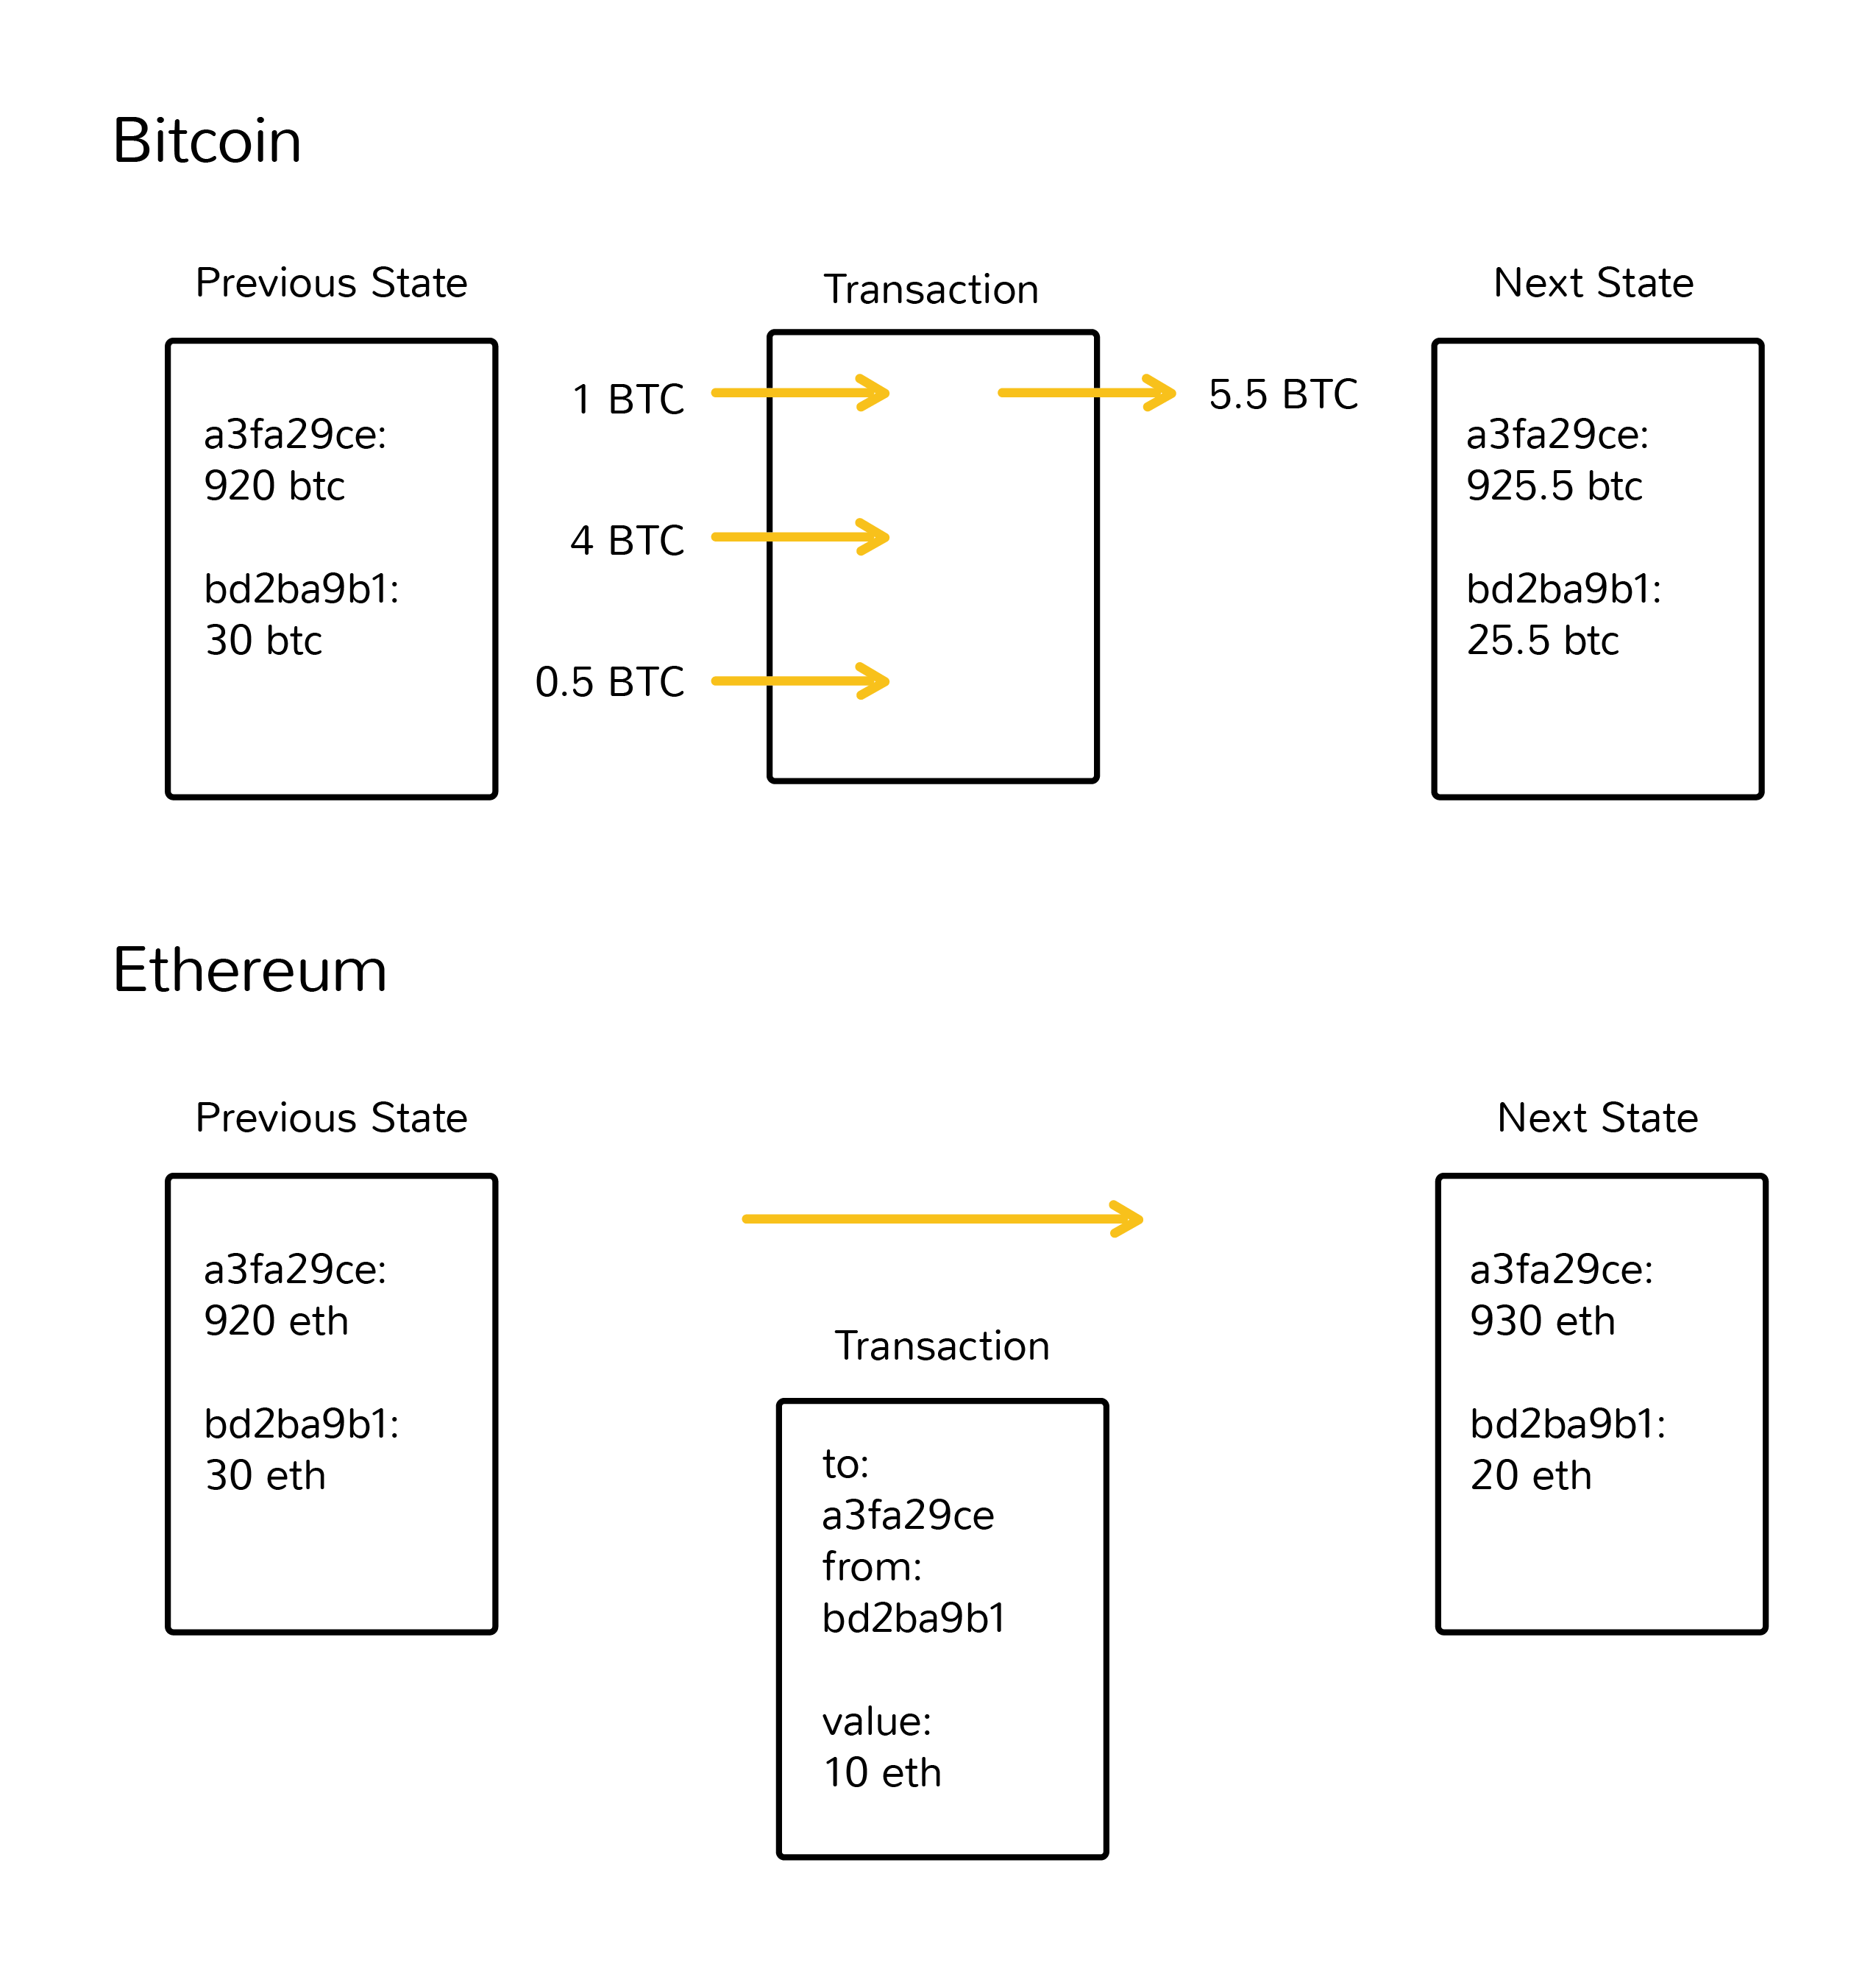
\includegraphics[scale=0.5]{images/statecoindesk.png}
    \caption{Diferencia del estado de las transacciones por Coindesk.}
    \label{fig:ethereum state transaction}
\end{figure}


\subsection{Lenguajes de programación para la EVM}
Los smart contracts de Ethereum pueden ser escritos en \textbf{Solidity}\cite{soliditylink} (un lenguaje de bibliotecas que posee similitudes con C y JavaScript), \textbf{Serpent}\cite{serpentlink} (similar a Python, pero deprecado), \textbf{LLL}\cite{llllink} (un lenguaje bajo nivel similar a Lisp), \textbf{Mutan}\cite{mutanlink} (basado en Go, pero también deprecado), \textbf{Vyper}\cite{vyperlink} (orientado a la investigación, fuertemente tipado, basado en Python, recursivo), y recientemente la empresa \textbf{BlockStack}\cite{blockstacklink} presentó \textbf{Clarity}\cite{claritylink} (tiene intencionado optimizar la predictibilidad y la seguridad).

Esto convierte a Solidity en el lenguaje más utilizado, o de facto, a la hora de desarrollar smart contracts en \textbf{Ethereum Network}\cite{ethereumhowlink}.


\section{Auditando blockchains}
Entonces, repasando un poco ahora que se posee la terminología necesaria: se puede desarrollar un smart contract en Solidity, que es compilado a bytecode, y si todo es correcto, será puesto en funcionamiento (\textit{deployado}) de manera inmutable a la blockchain. Allí todos los nodos que poseen máquinas virtuales tendrán una copia de ese contrato, y de ahora en más deberán llegar a un consenso en cuanto a si los interacciones que lo involucran y sus modificaciones de estado son correctos.

Entendiendo esto, se pueden definir las siguientes maneras de auditar una tecnología blockchain que utiliza smart contracts:
\begin{itemize}
    \item \textbf{Análisis estático al código}\newline
    Análisis al código mediante la automatización de herramientas que buscan patrones comunes susceptibles a errores y fallas de seguridad.
    \item \textbf{Análisis dinámico del contrato}\newline
    Analizar mediante cualquier medio el comportamiento del contrato, interactuando en vivo en la blockchain. Generalmente se replica en un entorno seguro, como en una red de testeo, conocidas como testnets.
    \item \textbf{Ingeniería inversa al bytecode deployado}\newline
    Analizar directamente el código resultante de la compilación, es decir el bytecode, lenguaje que interpreta la EVM. Generalmente se utiliza para observar si se introdujeron errores en el proceso de deployment, o para los contratos cuyo código fuente no se posee.
    \item \textbf{Verificación formal}\newline
    Es el mecanismo mediante el cual se prueba la correctitud de un contrato, basada en la verificación formal de lo que se supone que debería hacer. Una manera de realizar análisis estático pero sumamente compleja. Generalmente lo realiza quién lo desarrolla.
    \item \textbf{Ejecución simbólica}\newline
    Mecanismo para analizar un contrato con el fin de entender qué entradas estimulan qué partes de él.
\end{itemize}

Algunas de estas técnicas implican analizar directamente el bytecode como output del compilador de Solidity por ejemplo, o el bytecode del contrato deployado en la blockchain, por más que se posea el fuente.

¿Por qué se ofrece esta alternativa? Porque es lógico asumir luego de las declaraciones anteriores, que no se puede confiar en la manera en la que los compiladores optimizan o interpretan el código. Por eso es necesario comprobar que la salida interpretada por la EVM tiene de hecho la intención con la que fue diseñado.

\section{¿Por qué el compilador de Solidity?}
En el momento de la escritura de esta sección, la moneda que maneja la Ethereum Network ether, es decir 1 \textbf{ETH}, equivale a un total de \textbf{US\$}266.29. El volúmen de transacciones de ETH en dólares de las últimas 24 horas es de \textbf{US\$}8.584.415.157 o 939.202 BTC. Es decir, con la cotización del dólar en Argentina, equivale a un total de \textbf{AR\$}372.282.118.457,18\cite{coinmarketcap}
El \textbf{ether} no es el único bien que posee muchas transacciones diarias. También existen los tokens, que se pueden comprar con monedas. Una moneda opera independientemente, mientras que un token posee un uso específico en el ecosistema de un proyecto. Son creadas sobre la red de Ethereum, gestionadas mediante smart contracts. Algunos ejemplos y sus volúmenes en las últimas 24 horas de esta redacción son:

\begin{itemize}
    \item Dai: DAI \$22,038,619 USD 
    \item Maker: MKR \$1,514,750 USD 
    \item OmiseGo: OMG \$119,081,815 USD 
    \item Basic Attention Token: BAT \$66,837,473 USD
    \item 0x: ZRX \$17,960,636 USD 
    \item Augur: REP \$6,113,229 USD
    \item Usd Coin Classic: USDC \$177,029,191 USD
    \item Paxos Standard Token: PAX \$128,207,385 USD
    \item Status: SNT \$16,693,466 USD
    \item Golem: GNT \$1,843,572 USD 
    \item Decentraland: MANA \$10,516,180 USD
\end{itemize}


Esto no incluye otras plataformas de Ethereum paralelas como \textbf{EOS}, \textbf{Tron}, \textbf{IOST} o más, en donde algunos de sus volúmenes en las últimas 24 horas supera los miles de millones de dólares en sólo alguna de las aplicaciones que corren, como por ejemplo \textbf{TRONBet} para Tron, \textbf{dice2.win} para ETH, o \textbf{EOSJacks} para EOS\cite{dappradar}.

El interés que ha habido en este ambiente por la cantidad de dinero que manejan ha aumentado en gran cantidad desde sus comienzos. En el sitio de Ledger, fabricantes de billeteras digitales en hardware, muestran un diagrama de tiempo\cite{ledgerhackstime} con todos los hackeos que han recibido los sitios de intercambio (\textbf{exchanges}) desde sus comienzos. Los costos en pérdidas superan el billón de dólares en costos.

\subsection{Smart contract hacks}
En esta sección se presentan tres ejemplos de \textit{hackeos} de alto impacto, de los más populares que han acontecido desde el momento en el que se empezó a interactuar con Smart Contrats en la red de Ethereum.


\subsubsection{El DAO hack}
Una \textbf{DAO} es una Organización Autónoma Descentralizada o una organización que se ejecuta a través de smart contracts. Las decisiones se toman digitalmente mediante la votación de los miembros de la organización, eliminando la necesidad de documentos y personas que gobiernan y, en consecuencia, un sistema de control descentralizado.

En este caso, la DAO comprendía una serie de contratos inteligentes destinados a democratizar cómo se financiaban los proyectos de Ethereum. Un hacker, al darse cuenta de una vulnerabilidad, robó USD\$ 3.6 millones de Ethers mediante la explotación de una función (\textit{fallback}) en el código que fue expuesto a una vulnerabilidad conocida como \textit{reentrancy} (re-entrada). Para recuperar los fondos, se tuvo que tomar una dura decisión, atentando contra la fe de los usuarios, que condujo a la creación de Ethereum Classic y Ethereum como dos cadenas separadas.\cite{daoattack}


\subsubsection{Multi-firma Wallet hack de Parity}
La empresa \textbf{Parity} hizo “billeteras” (\textit{wallets}) de software multi-firma (multi-sig) para la gestión de la criptomoneda Ether. Estas wallets multi-sig eran contratos inteligentes disponibles en una base de código abierto que requerían más de una firma digital (clave privada) antes de que el Ether asociado con ellos pudiera ser aprobado para su transferencia.
Un hacker desconocido robó 150,000 Ethers, alrededor de USD\$30.000.000 en ese momento\cite{parityheist}.

\subsubsection{Wallets de Parity congeladas por un usuario}
Apenas unos meses después del hackeo en julio de 2017, un usuario explotó accidentalmente una vulnerabilidad en el código de la biblioteca de Parity para las wallets multi-sig, congelando más de 513.774,16 ETH, lo que representaba en esa época más de USD\$106.864.992\cite{parityfreeze}.\newline

\textbf{En conclusión},\textit{ no solo se tiene la importancia de auditar un compilador por las razones mencionadas anteriormente, sino que al auditar un compilador como el de Solidity, se estaría auditando un compilador cuyo código emitido e inmutable corre en todas las máquinas virtuales de todos los nodos de una red. Es decir que si se encuentra la manera de, vulnerar los contratos para obtener su balance, o la manera de emitir un mensaje que detenga el funcionamiento de toda la red, sería catastrófico.}

% \chapter{Estado del arte}
% Teniendo en cuenta que no existe una teoría o mecanismo formalmente establecido para la auditoría específica de compiladores, más allá de lo presentado en el capítulo 2, podría pensarse que existen varias maneras de realizar dicha tarea.\\

Una de las maneras más sencillas de auditar el proceso, de transformar el código fuente a un ejecutable, sería generar binarios para el mismo código fuente de un lenguaje, mediante distintos compiladores, y comparar los resultados.\\

También se podría generar un mismo compilador, con distintos compiladores, para una misma arquitectura, y observar si las distintas optimizaciones aplicadas sobre el mismo compilador hacen que las generaciones realizadas por el resultante difieran tras realizarle un análisis estático.\\

Clarificación con un ejemplo. Como primer paso, se compila el código fuente para \textbf{gcc} utilizando dos compiladores distintos, \textbf{gcc} y \textbf{clang}; por lo tanto, ambos deberían devolver un ejecutable cada uno, en este caso \textbf{gcc-gcc} y \textbf{gcc-clang}. Luego, una de las maneras más sensatas de corroborar que sus lógicas son idénticas es compilar el mismo archivo con ambos compiladores resultantes, y comparar sus resultados. Como la lógica, en teoría, es la misma, ambos deberían manifestarse de la misma manera, y de hallar alguna diferencia en el programa resultante se comprobaría que alguno falló, probablemente por optimizaciones con comportamiento inesperado.\\

A continuación se presenta una selección de proyectos con las propuestas más interesantes que se encuentran en el marco de esta investigación. La mayoría de las propuestas están presentadas mediante una combinación de traducciones, adaptaciones, e interpretaciones de los artículos originalmente publicados, incluyendo un análisis de sus herramientas, en el caso de estar públicas.

\section{CSMith (2009-2013)}
\textbf{CSmith} es una herramienta de generación de casos de test randomizados, utilizada para encontrar errores en compiladores durante 5 años. A diferencia de herramientas antecesoras, Csmith genera programas que cubren un gran subconjunto del lenguaje C. Evita los comportamientos indefinidos y no especificados que podrían destruir la habilidad de encontrar automáticamente bugs por código erróneo. \\

Todos los compiladores que se testearon con esta herramienta se detuvieron inesperadamente (crash), y también silenciosamente generaban código erróneo cuando eran presentados con input válido.\\

\begin{lstlisting}[language={c}, label={lst:gcc vulnerable code}, caption={Código que produjo bug en GCC}, captionpos={b}, frame={shadowbox}]]
int foo (void) {
    signed char x = 1;
    unsigned char y = 255;
    return x > y;
}
\end{lstlisting}

El código del recuadro\ref{lst:gcc vulnerable code} pertenece a un bug hallado en una versión de GCC incluído con Ubuntu Linux 8.04.1 para x86. En todos los niveles de optimización compilaba esa función  de forma que en su ejecución retorne el valor "1"; cuando el resultado correcto es "0". Lo que sucedió fue que el compilador de Ubuntu había sido fuertemente modificado a través de lo que se conoce como “parche”, ya que la versión base de GCC no poseía ese bug\cite{Yang:2011:FUB:1993316.1993532}.\\

Csmith genera un programa en C; luego un código de prueba (conocido como "arnés de prueba") compila ese programa utilizando diversos compiladores, ejecuta los ejecutables, y compara las salidas. A pesar de que esta estrategia ya había sido utilizada previamente \cite{Eide:2008:VM:1450058.1450093}\cite{McKeeman98differentialtesting}\cite{Sheridan2007c99comparison}, las técnicas de generación de Csmith, para ese momento, avanzaron sustancialmente el estado del arte generando programas aleatorios que son expresivos—conteniendo código complejo utilizando muchas de sus características—mientras también aseguraban que cada programa generado tenga una sola interpretación. Para poder hacer esto, un programa no debe poder ejecutar ningún tipo de comportamientos indefinido, ni debe depender de ninguno de los 52 tipos de comportamiento no especificado que están descritos en el estándar C99\cite{openstdc99}.\\

Los autores de la herramienta claman que Csmith es efectiva para buscar bugs, en parte porque genera casos de testeo que exploran combinaciones atípicas del lenguaje. Que sea código atípico no significa que no sea importante, sin embargo; no se encuentra bien representado en las suites de testeo existentes. Los desarrolladores que se aventuran fuera de los caminos más testeados que representan lo que podría denominarsela "zona de confort" del compilador -- por ejemplo escribiendo un kernel o sistemas embebidos, utilizando opciones de compilación esotéricas (de uso extremadamente específico), o generando código automáticamente -- pueden encontrarse bugs bastante frecuente.\\

Este proyecto comenzó como un \textbf{fork} (bifurcación) de \textbf{Randprog}\cite{randprog}, un proyecto ya existente que genera programas aleatorios en C de 1600 líneas de código. En sus trabajos tempranos extendieron y adaptaron Randprog para encontrar bugs en la parte de la traducción de accesos a objetos calificados de volátiles, lo que dió como resultado a un programa de 7000 líneas de código. 
Los autores convirtieron Randprog en Csmith, un programa C++ de 40,000 líneas para generar programas de C aleatorios. En comparación con Randprog, Csmith puede generar programas de C que utilizan una gama mucho más amplia de características de C, incluido el flujo de control complejo y estructuras de datos como punteros, matrices y estructuras.\\

El programa Csmith utiliza pruebas diferenciales aleatorias. Las pruebas aleatorias\cite{pinho2006reliable}, también llamadas fuzzing\cite{Miller:1990:ESR:96267.96279}, consisten en un método de test black box en el que las entradas de prueba se generan aleatoriamente. Las pruebas diferenciales aleatorias\cite{McKeeman98differentialtesting} tienen la ventaja de que no se necesita un oráculo (principio heurístico o mecanismo por el cual podremos reconocer un problema, y determinar si es correcto o no). para los resultados de las pruebas. Explota la idea de que si uno tiene implementaciones deterministas múltiples de la misma especificación, todas las implementaciones deben producir el mismo resultado de la misma entrada válida. Cuando dos implementaciones producen salidas diferentes, una de ellas debe ser defectuosa. Dadas tres o más implementaciones, un evaluador puede usar el voto para determinar heurísticamente qué implementaciones son incorrectas. La Figura \ref{fig:csmith compilers} muestra cómo usaron estas ideas para encontrar errores de compilación.\\

\begin{figure}[h]
    \centering
    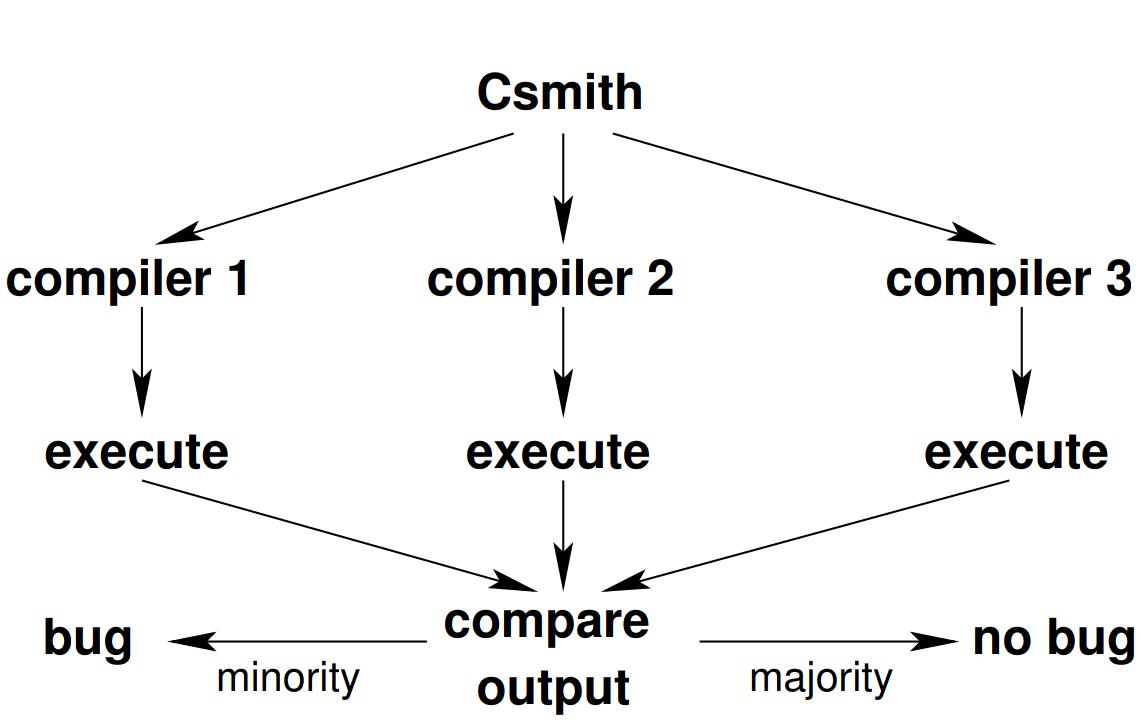
\includegraphics[scale=0.3]{images/csmith1.png}
    \caption{Ejecución en distintos compiladores}
    \label{fig:csmith compilers}
\end{figure}

\subsection{Resultados obtenidos}
Desde el año 2009 al 2013 encontraron 476 bugs en GCC\cite{gccbuglistcsmith} y LLVM\cite{llvmbuglistcsmith}.\\

La lista de bugs es accesible desde su repositorio\cite{bugsreportedcsmith} en github, también desde el sitio del departamento de Ciencias de la computación de UTAH.\\

El proceso de testear al azar es útil pero posee desventajas: no se puede saber cuándo dejar de testear; optimizar las probabilidades no es trivial; generar salidas expresivas que sean realmente correctas no es sencillo; y finalmente, es limitado al lenguaje. Csmith declara ser el ataque que utiliza como técnica al \textit{fuzzing}, como el más extensivo en comparación con los compiladores de su época.\\

\textit{Resumidamente, la función de CSMith es aplicar técnicas de fuzzing el compilador utilizando programas generados al azar basados en la gramática, del lenguaje C, interpretando los resultados.}

\section{DeepSmith (2018)}
Los autores de la herramienta presentan \textbf{DeepSmith}\cite{Cummins:2018:CFT:3213846.3213848}, como un novedoso enfoque de aprendizaje automático para acelerar la validación del compilador a través de la inferencia de modelos generativos para las entradas del compilador. Su enfoque infiere un modelo, aprendido de la estructura de código real basado en un gran códigos open source. Luego, utiliza el modelo para generar automáticamente decenas de miles de programas realistas. Finalmente, aplican metodologías de pruebas diferenciales establecidas para exponer errores en los compiladores.\\

Se ha aplicado este enfoque al lenguaje de programación \textbf{OpenCL}, exponiendo automáticamente los errores en los compiladores de OpenCL con poco esfuerzo de su lado. En 1.000 horas de pruebas automatizadas de compiladores comerciales y de código abierto, descubrieron errores en todos ellos.

\subsection{Comparación con CSmith}
CSmith se desarrolló a lo largo de los años y consta de más de 41k líneas de código C ++ escritas manualmente. Al unir estrechamente la lógica de generación con el lenguaje de programación de destino, cada característica de la gramática debe diseñarse de forma minuciosa y experta para cada nuevo idioma de destino.\\

Por ejemplo, adaptar CSmith de C a \textbf{OpenCL}\cite{Boujarwah1997CompilerTC} - una tarea que parecería ser simple - les tomó 9 meses y 8k líneas adicionales de código. Dada la dificultad de definir una nueva gramática, generalmente solo se implementa un subconjunto del lenguaje.\\

Su metodología utiliza los avances recientes en \textit{deep learning} (conjunto de algoritmos de \textit{machine learning}) para construir automáticamente modelos probabilísticos de cómo los humanos escriben el código, en lugar de definir meticulosamente una gramática con el mismo fin. Al entrenar una red neuronal profunda en un corpus de código \textit{manualmente escrito}, es capaz de inferir tanto la sintaxis como la semántica del lenguaje de programación. El enfoque de los autores de la herramienta esencialmente enmarca la generación de programas aleatorios como un problema de modelado de lenguaje. Esto simplifica y acelera enormemente el proceso.\\

Lo más interesante de esto es que las herramientas \textit{infieren la sintaxis, la estructura y el lenguaje de programación}. Utilizan ejemplos del mundo real, no a través de una gramática definida por expertos. El tamaño promedio de los casos de prueba es dos órdenes de magnitud más pequeño que el estado del arte, sin ningún proceso de reducción costoso, y toma menos de un día para entrenar.\\

Los autores descubrieron un número similar de errores que el estado del arte, pero también encontraron errores que el trabajo anterior no pudo, cubriendo más componentes del compilador. Y en el modelado de código manualmente escrito, sus casos de prueba son más interpretables que otros enfoques.\\

\begin{figure}[h]
    \centering
    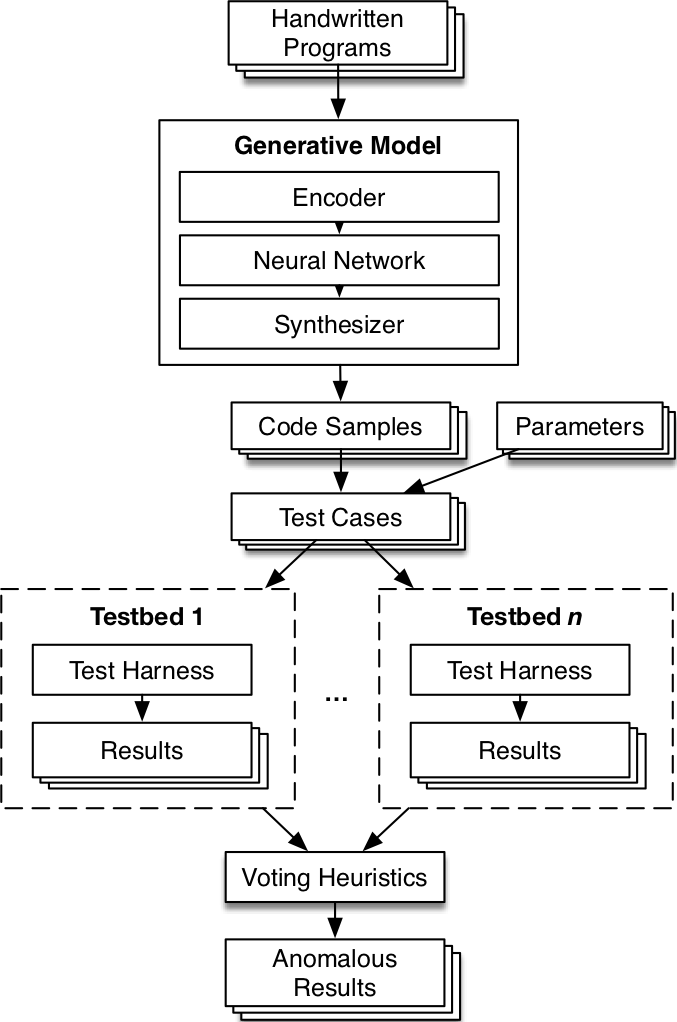
\includegraphics[scale=0.5]{images/deepsmith1.png}
    \caption{Arquitectura de DeepSmith}
    \label{fig:deepsmith architecture}
\end{figure}


\subsection{Extensibilidad del modelado de lenguajes}

Una gran parte de la arquitectura de DeepSmith es independiente del lenguaje;ya que solo requiere un corpus, un codificador y un arnés para cada nuevo lenguaje. Esto potencialmente reduce  significativamente la barrera de entrada en comparación con los fuzzers basados en gramática anteriores (la gran mayoría). Para explorar esto, deciden intentarlo con un lenguaje reciente, siendo este Solidity.\\

La razón de seleccionar a Solidity, se debe a que posee menos de cuatro años, carece de gran parte de las herramientas de lenguajes de programación más establecidos y los errores explotables pueden socavar la integridad de la blockchain y provocar transacciones fraudulentas. 

\subsection{Resultados iniciales}
La investigación se realizó ejecutando el bucle del arnés y el generador durante 12 horas en cuatro bancos de pruebas: el solc de compilación de referencia de Solidity con optimizaciones activadas o desactivadas, y solc-js, que es una versión compilada por Emscripten del compilador de solc.\\

Sus resultados se resumen en la tabla que muestra la Figura \ref{fig:deepsmith solc}.

\begin{figure}[h]
    \centering
    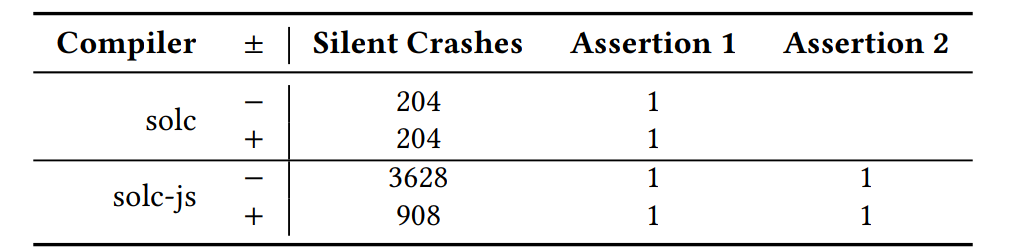
\includegraphics[scale=0.3]{images/deepsmithsolc.png}
    \caption{Resultados de testear solc y solc-js.}
    \label{fig:deepsmith solc}
\end{figure}


Los resultados de la investigación demostraron numerosos casos en los que el compilador se bloquea silenciosamente y dos aserciones distintas del compilador. El primero se debe a la falta de manejo de errores en las características del idioma (este problema es conocido por los desarrolladores). La fuente de la segunda afirmación es el tiempo de ejecución de JavaScript y se activa solo en la versión Emscripten, lo que sugiere un error en la traducción automática de LLVM a JavaScript.\\

La extensión de DeepSmith a una segunda programación requirió 150 líneas adicionales de código (18 líneas para el generador y el codificador, el resto para el arnés de prueba) y tomó aproximadamente un día. Dada la reutilización de los componentes básicos de DeepSmith, hay un costo decreciente con la adición de cada nuevo idioma. Por ejemplo, el codificador y reescritura de OpenCL, implementado utilizando LLVM, podría adaptarse a C con cambios mínimos. Dado el bajo costo de la extensibilidad, los autores de la herramienta creen que estos resultados preliminares indican la utilidad de su enfoque para simplificar la generación de casos de prueba.

\subsection{Trabajos relacionados}
La generación aleatoria de casos de prueba es un enfoque bien establecido para el problema de validación del compilador. Los enfoques anteriores se examinan en \textit{Compiler test case generation methods: a survey and assessment}\cite{Boujarwah1997CompilerTC}, \textit{Survey of Compiler Testing Methods}\cite{Kossatchev2005CompilerTM} y se contrastan empíricamente en \textit{An empirical comparison of compiler testing techniques}\cite{ComparisonCompilerTechniques}. La principal pregunta de interés es cómo generar de manera eficiente los códigos que desencadenan errores.\\

Hay dos enfoques principales: la generación de programas, donde las entradas se sintetizan desde cero; y la mutación del programa, donde los códigos existentes se modifican para identificar comportamientos anómalos.

\subsection{Programa de generación}
En el trabajo fundacional sobre pruebas diferenciales para compiladores, McKeeman et al. presentan generadores actuales capaces de enumerar programas de una variedad de calidades, desde secuencias ASCII aleatorias hasta programas conformes con el modelo C\cite{McKeeman98differentialtesting}. Los trabajos posteriores han presentado generadores cada vez más complejos que mejoran en alguna métrica de interés, generalmente expresividad o probabilidad de corrección. CSmith\cite{Yang:2011:FUB:1993316.1993532} es un generador ampliamente conocido y efectivo que enumera programas al vincular funciones de lenguaje combinadas con poca frecuencia. Al hacerlo, produce programas correctos con un comportamiento claramente definido pero una funcionalidad muy poco probable, lo que aumenta las posibilidades de desencadenar un error.\\

Lograr esto requirió un extenso trabajo de ingeniería, la mayoría no se puede transportar a otros idiomas, e ignorar algunas características del idioma. Los generadores subsiguientes influenciados por CSmith, como Orange3\cite{Nagai:Hashimoto:Ishiura}, se enfocan en características y tipos de errores más allá del alcance de CSmith, errores aritméticos en el caso de Orange3.\\

Glade\cite{Glade:Bastani:Sharma:Aiken:Liang} deriva una gramática de un corpus de programas de ejemplo. La gramática derivada se enumera para producir nuevos programas, aunque a diferencia de nuestro enfoque, no se aprende ninguna distribución sobre la gramática; la enumeración del programa es uniformemente aleatoria.

\subsection{Programa de mutación}
La prueba de entradas de módulo de equivalencia (EMI)\cite{Le:Afshari:Su:Modulo}\cite{Sun:Le:Su:Mutation} sigue un enfoque diferente para la generación de casos de prueba. Comenzando con el código existente, inserta o elimina instrucciones que no se ejecutarán, por lo que la funcionalidad debe seguir siendo la misma. Si se ve afectado, se debe a un error del compilador. Si bien es una técnica poderosa capaz de encontrar errores difíciles de detectar, se basa en tener una gran cantidad de programas para mutar. Como tal, todavía requiere un generador de código externo. De manera similar a CSmith, EMI favorece los programas de prueba muy largos.\\

LangFuzz\cite{Holler:Herzig:Zeller:Fragments} también usa la mutación, pero lo hace insertando segmentos de código que previamente han expuesto errores. Esto aumenta las posibilidades de descubrir vulnerabilidades en los motores de lenguaje de scripting.\\

La enumeración de programas esqueléticos\cite{Zhang:Sun:Su:Skeletal} funciona nuevamente al transformar el código existente. Identifica patrones algorítmicos en piezas cortas de código y enumera todas las posibles permutaciones del uso variable. Comparado con todo esto, su enfoque de fuzzing es de bajo costo, fácil de desarrollar, portátil, capaz de detectar una amplia gama de errores y enfocado por diseño a los errores que es más probable encontrar en un escenario de producción.

\subsection{Aprendizaje automático}
Existe un creciente interés en aplicar el aprendizaje automático a las pruebas de software. Más parecido a su trabajo es Learn \& fuzz\cite{Godefroid:Peleg:Singh:LearnAndFuzz}, en el cual una red LSTM se entrena a través de un conjunto de archivos PDF para generar entradas de prueba para el renderizador Microsoft Edge, produciendo un error. A diferencia de las pruebas de compilación, los casos de prueba de PDF no requieren entradas ni procesamiento previo del cuerpo de entrenamiento.\\

Skyfire\cite{Wang:Chen:Wei:Liu:Skyfire} aprende una gramática probabilística sensible al contexto sobre un corpus de programas para generar semillas de entrada para pruebas de mutación. Se muestra que las semillas generadas mejoran la cobertura del código de AFL\cite{AFL} cuando confunden los motores XSLT y XML, aunque las semillas no se usan directamente como casos de prueba. El aprendizaje automático también se ha aplicado a otras áreas, como la mejora de los analizadores estáticos de detección de errores \cite{Heo:Oh:Yi:Unsound}\cite{Koc:Saadatpanah:Jeffrey:Porter:False} la reparación de programas\cite{Koukoutos:Raghothaman:Kneuss:Kuncak}\cite{White:Tufano:Martinez:Monperrus}, la priorización de los programas de prueba\cite{Chen:Bai:Hao:Xiong:Zhang}, la identificación de buffer overruns (sobrecargas de búfer)\cite{Choi:Jeong:Oh:Choo:BufferOverruns} y el procesamiento de informes de errores\cite{Xuan:Ming:Buggy}\cite{Lam:Anh:Nguyen:Nguyen:DeepLearning}. Según el conocimiento de los autores, ningún trabajo hasta el momento ha tenido éxito en la búsqueda de errores de compilación al explotar la sintaxis aprendida del código fuente extraído para la generación de casos de prueba. Aparentemente el trabajo de estos autores es el primero en hacerlo.

\section{Serpent by Zeppelin (Jul 2017)}

La empresa Zeppelin, crea herramientas para el desarrollo seguro, deployment y operación de sistemas descentralizados. También ayudan a compañías a securizar sus sistemas blockchain realizando auditorías.\\

La empresa Augur (un servicio de apuestas descentralizado) los contrató para realizarle una auditoría a Serpent, un compilador de un lenguaje Python-style que compila a EVM. El interés de Augur en esta auditoría está dado por razones propias, tuvieron un inconveniente de seguridad por utilizar este lenguaje. El código del proyecto se puede ver aún en su repositorio de GitHub\cite{SerpentRepository}.\\

\begin{displayquote}
    \textit{"Hemos encontrado que el proyecto Serpent es de muy baja calidad. No se ha testeado, hay muy poca documentación y el diseño del lenguaje es muy defectuoso. La serpiente no debe considerarse segura de usar a menos que se solucionen muchos problemas críticos."}
    \newline{\null\hfill -- Zeppelin Research team}
\end{displayquote}

En su publicación\cite{SerpentCompilerAuditZep}, la introducción a los resultados del reporte también es utilizada como conclusión al final del mismo. El contenido de ella es una la lista con los problemas apuntando directamente al documento original que posee detalle técnico.\\

El reporte original menciona que su estrategia fue analizar el código C++ del compilador, sumado a revisar documentación, ejemplos, y herramientas recomendadas para trabajar con los contratos de Serpent. Realizaron diversos contratos de ejemplo minimales, para verificar y exponer los problemas que encontraron. Analizaron el código assembler tanto en LLL (Lisp Like Language, un lenguaje con un nivel de abstracción superior a la EVM, pero considerado assembler) como en la EVM, así como también su comportamiento en ejecución.\\

El análisis no explica metodologías ni tecnologías aplicadas a obtener a estos resultados. En base a todo lo observado el autor concluye que fue se trata de un proceso manual, poco automatizado, de un gran equipo. Sin embargo el acercamiento que la empresa tomó, a nivel proyecto, parece mucho más interesante que simplemente crear una herramienta, utilizar una ya existente sin explicar cómo utilizarla, o publicar los resultados sin establecer contacto con el equipo del producto analizado. Tal vez sea una diferencia destacable entre proyectos de grado y un contrato empresarial.
Fué la primera auditoría que llamó la atención del autor en su momento, y mostró tanto la importancia como el estado inmaduro del mercado en este tipo de tecnologías.\\ 

Lamentablemente la auditoría fue realizada sobre un proyecto que aparenta haber sido descontinuado mientras se publicaba ese reporte. El reporte fue presentado en Julio del 2017, y las últimas actualizaciones a Serpent fueron realizadas meses antes. Actualmente se encuentra obsoleto y sin aplicar los cambios recomendados por el equipo.


\section{Solidity by Coinspect (Nov 2017)}
Nuevamente Augur contrató otro equipo de investigadores, esta vez a Coinspect, para realizar una auditoría al compilador de Solidity.\\

Coinspect, es un equipo reconocido por sus trabajos específicamente en el ambiente de la cyber seguridad. Entendiendo esto, no es extraño encontrar en la introducción de la publicación\cite{SolidityCompilerAuditReport} un poco más de detalle\cite{SummaryCoinspectReport} sobre lo que esperan encontrar o qué piensan en buscar relacionado en términos de seguridad.\\

El equipo de Coinspect analizó la herramienta Solidity con la posibilidad de encontrar fallas del siguiente estilo:
\begin{itemize}
    \item Reducción de la seguridad de los contratos desplegados.
    \item Resultado en comportamiento no determinista.
    \item La ejecución de código malintencionado o que se bloquee al analizar el código fuente de un contrato en Solidity especialmente diseñado.
    \item Agotamiento de recursos durante la compilación, ya sea CPU, memoria o disco.
    \item Código compilado que consume una cantidad no constante de gas (por ejemplo, según los argumentos), donde el programador habría esperado un costo constante.
    \item Facilitando código malicioso (troyanos en código abierto).\newline
\end{itemize}

También buscaron vulnerabilidades comunes a vectores en aplicaciones de software:
\begin{itemize}
    \item Validación de entrada.
    \item Prevención de denegación de servicio (DoS).
    \item Prevención de la fuerza bruta.
    \item Divulgación de información.
    \item Vulnerabilidades de corrupción de memoria: buffer overflows, format strings por el usuario.
    \item Integer overflows/underflows.
    \item Vulnerabilidades de gestión de punteros: double free, user after free.
\end{itemize}


En cuanto a los resultados, exceptuando uno sólo de los problemas reportados que parece haber sido hallado mediante un proceso manual, el autor se atrevería a decir que el resto pertenecen a una clásica familia resultante de aplicar técnicas de fuzzing.\\

La diferencia principal que se podría hacer, sobre los análisis de Serpent y Solidity, es que Coinspect se enfoca principalmente en el hallazgo de vulnerabilidades y Zeppelin a problemas de diseño e implementación, los cuales a su vez pueden tener implicancias de seguridad.\\

Hay que tener en cuenta que que se hace imposible comparar con objetividad los procesos de cada equipo, dado que están meramente basadas en los resultados de cada investigación, y no se están teniendo en cuenta las herramientas disponibles, ni los recursos económicos o el tiempo que poseyó cada equipo al momento de realizarlas.\\

\section{Solidity by Ethereum Foundation}

Para situarse en contexto, el compilador de Solidity junto con su lenguaje fueron impulsados por la Ethereum Foundation. Su código está disponible en GitHub\cite{SolidityGitHub} desde sus comienzos, donde realizan releases periódicamente, tienen su documentación en ReadTheDocs\cite{ReadTheDocsSolidity}, y una amplia comunidad que colabora con el proyecto.\\

Si bien al momento de esta investigación no parecen aplicar seguridad a su SDLC, en su repositorio dicen realizar testing y fuzzing antes de cada release. Adicionalmente en su documentación se poseen categorías útiles con la intención de reducir las fallas en el código. Algunos ejemplos son patrones de diseño, código de estilo, consideraciones de seguridad, reproducción de testing, y una explicación de cómo utilizar el fuzzer que está incluido en el proyecto.\\

Varios de los bugs reportados por el equipo de Coinspect siguen sin estar corregidos, y no es posible distinguir en el sistema de reportes de tickets de github, qué bugs corresponden a su suite de testing, y de qué manera se han encontrado. Tal vez muchos errores no llegan a ser publicados mediante commits porque son testeados localmente, y esa información no se encuentra visible al público. El sitio solfuzz.ethdevops.io\cite{SolfuzzSite} solía dar estadísticas de los resultados encontrados por el fuzzer incorporado pero en el momento de este análisis se comprobó que ha dejado de funcionar hace tiempo.\\

Podrá no ser una solución similar a las demás, ya que no se dedican específicamente a aplicar seguridad o auditar el proyecto. Pero todas las soluciones apuntan a lo mismo, securizar los smart contracts através del compilador. Ésta es una tarea que principalmente el equipo de Solidity debería liderar ya que es su responsabilidad tomar los recaudos necesarios a través de su ciclo de desarrollo para proveer un servicio seguro.

\section{Discusión sobre las soluciones presentadas}
Mientras más eficiente sea la herramienta para analizar un compilador, más acoplada a su gramática deberá ser, y como consecuencia serán menos abarcativas. La adaptación de estas herramientas para poder migrar entre lenguajes es sumamente costosa.\\

En el caso de DeepSmith, los autores de la herramienta lograron aplicar su funcionalidad partiendo desde OpenCL hasta Solidity sin demasiado esfuerzo. Sin embargo, los testeos sobre los compiladores de Solidity fueron de los más breves y menos explorados que realizaron. No se buscaron impactos reales ni se hizo un chequeo sustancial sobre los hallazgos.\\

La problemática que se trata de presentar no es que el fuzzing no funciona, sino que no forman parte directa de realizar una auditoría. Se presentan como herramientas, analizan los proyectos, en este caso compiladores, y dan por finalizada la investigación. Su propósito no es encontrar y analizar las vulnerabilidades, sino proveer una herramienta para hacerlo.\\

Las dos propuestas que poseen un valor destacable, son las realizadas por las dos empresas previamente mencionadas, Coinspect y Zeppelin. Aún así son un paso accesorio a las herramientas presentadas, sólo que la herramienta en cuestión es un equipo en vez de un sólo software.\\

\textit{Las sugerencias incorporadas al reporte de Serpent por parte del equipo de Zeppelin fueron de gran motivación para realizar este proyecto.}\\

Al momento de la redacción de este documento, no se encuentra disponible una herramienta para analizar el código de compilador y entender cómo podría influir al lenguaje que ésta interpreta. En el caso de Solidity tampoco hay una gramática oficial definida de manera reutilizable, ya que el scanner no está basado en una gramática estándar, sino que está diseñada su lógica dentro del mismo parser.
Teniendo en cuenta lo descrito en el capítulo anterior, se puede concluir que las alternativas provistas e históricas en el estado del arte no son soluciones suficientes o aplicables para concluir un análisis completo, o mejor dicho una auditoría completa, al proyecto en cuestión, Solidity.

% \chapter{Método propuesto}
% \section{Introducción}

El objetivo de la metodología descripta en este capítulo consiste en revisar el compilador y lenguaje de Solidity, analizar su diseño general y arquitectura, y reportar potenciales vulnerabilidades de seguridad que puedan llegar a comprometer el código compilado. En este capítulo se describe el trabajo realizado presentando ejemplos de observaciones en áreas específicas del código que presentan problemas concretos, así como también observaciones generales que atraviesan el proyecto entero, que puede mejorar su calidad como un todo.\\

Se puede interpretar a la metodología como una auditoría abarcativa, no sólo de seguridad, sino en todos los aspectos que permitan encontrar problemas. No es menor resaltar que cualquier problema en este contexto puede ser considerado un potencial impacto de seguridad.\\

El método propuesto no tiene intención de destacarse por utilizar características novedosas a nivel tecnológico o introducir nuevos procesos. De hecho todo lo que se realizará en esta sección, no es más que, en distintas medidas, una conjunción de los dos capítulos anteriores, y es por eso que parece importante hacer énfasis en este tipo de propuestas, ya que están al alcance del estado del arte.\\

La razón de centrar el foco de investigación en un proyecto open source, que posee instrucciones sobre cómo construirlo, y una documentación extensa, es para presentar una situación favorable y menos limitante para realizar una auditoría. No obstante, poseer esta situación lo hace más complejo y desafiante, ya que se puede analizar desde todas las perspectivas posibles.\\

Su código está disponible online, y se ha decidido congelar el repositorio en la última versión estable a la hora de realizar esta investigación.


\section{Alcance de la auditoría}

El código auditado puede encontrarse en su repositorio público de GitHub ethereum/solidity\cite{SolidityGitHub}, y la versión utilizada para el análisis se encuentra en el \textit{tag} v0.4.24\cite{SolidityGitHub0424}, commit: \texttt{e67f0147998a9e3835ed3ce8bf6a0a0c634216c5}.\\

La auditoría contendrá un profundo análisis, diseño e implementación de la herramienta, apuntando a asesorar su calidad e investigar problemas potenciales que pueden surgir mediante su utilización.\\

Estas actividades incluyen revisar las etapas de \textit{parsing}, análisis, optimización, código de generación. La auditoría cubrirá el código ensamblador generado para la \textit{EVM}, \textit{ABIs} (Application Binary Interface), y Solidity con código intermedio \textit{Yul} de manera \textit{inline}.\\

No se cubrirá la generación de código \textit{eWASM} (Ethereum Flavored WebAssembly), las características relacionadas al lenguaje \textit{LLL} (lenguaje de bajo nivel para la \textit{EVM} con una sintaxis de expresiones-s ), las características experimentales, y las herramientas de verificación formal incluídas en el proyecto.\\

El proyecto no parece integrar la seguridad como componente activo en su ciclo de desarrollo. Incluye un componente para aplicar técnicas de \textit{fuzzing} y una suite de testeo. Estos no serán analizados con detenimiento pero de todos modos se verá cuál es su real interacción con el compilador.

\section{Metodología }
\label{chap:metodo:metodologia}
Para estos casos, siempre es mejor realizar una revisión manual de código, y como tal se debe comenzar con un modelado de amenazas o al menos entrevistas a los desarrolladores para tener un entendimiento de la arquitectura de la aplicación, su superficie de ataque, así como también las técnicas de implementación.\\

Es por eso que durante toda la auditoría se mantuvo siempre al menos un canal de comunicación abierto con el equipo encargado del proyecto. Se utilizaron servicios de mensajería\cite{GitterLink} para mantener un diálogo específicamente para detalles asíncronos sobre dudas puntuales, frecuentemente relacionadas a la información presentada en el repositorio de \textit{GitHub}.\\

\textit{GitHub} como herramienta fue utilizada en el proyecto como medio de intercambio de información de una manera más acoplada al proyecto, teniendo la posibilidad de continuar involucrando a la comunidad activa.\\

Finalmente para partes del código difíciles de comprender, se realizaron \textit{walkthroughs} (guías destinadas a mejorar el entendimiento del proyecto) mediante videollamadas en una herramienta de videoconferencia\cite{MeetLink}.\\ 

Se utilizó un conjunto de las estrategias de auditoría de código con propósitos bien definidos. Por ejemplo, la \textit{generalización de diseño} aplicada a analizar la arquitectura del compilador; \textit{puntos candidatos} para posibles problemas en las etapas de parsing y optimización; y \textit{compresión de código} basados en hallazgos mediante técnicas de \textit{black box} o \textit{testing} manual. Para una representación gráfica aproximada ver Figura \ref{fig:metodologia}.\\

\begin{figure}[ht]
    \centering
    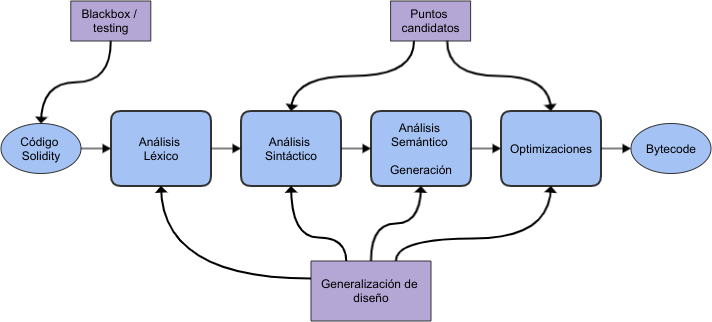
\includegraphics[scale=0.5]{images/methodology.png}
    \caption{Estrategias aplicadas, visualización.}
    \label{fig:metodologia}
\end{figure}

A grandes rasgos, se pretendió:
\begin{itemize}
    \item Cubrir un análisis general del proyecto en todos los aspectos del mismo, desde cómo está conformado el equipo que lo mantiene hasta las tecnologías que se utilizan.
    \item Realizar revisión de código en los puntos candidatos y en los lugares en donde se han  producido fallos en las pruebas de \textit{black box}.
    \item Auditar las distintas etapas del compilador a nivel general, buscando que la arquitectura del compilador contemple las etapas estándar.
    \item Revisar el diseño del lenguaje y su instrumentación para verificar que la instrumentación sea consistente con la especificación del diseño del lenguaje.
    \item Revisar la configuración de testeo para detectar posibles fallos en los códigos de testeo del propio proyecto.
    \item Aplicar técnicas de black box para identificar el lugar del fallo y el lugar y la magnitud del impacto del mismo.
    \item Analizar la salud del proyecto para hallar posibles defectos como compatibilidad hacia atrás, aspectos no contemplados, información inconsistente y sin tratamiento en los repositorios, entre otros.
    \item Revisión de problemas previamente reportados para asegurar el tratamiento y seguimiento de temas ya identificados.
    \item Análisis de la documentación para verificar la consistencia entre la documentación y los aspectos de sintaxis, semántica y pragmática del compilador.
\end{itemize}
\bigskip

Finalizar una auditoría no consta únicamente de entregar lo hallado de manera descriptiva. Se cumple un rol muy importante a la hora de presentar los resultados, ya que sin alternativas, soluciones o sin mantener un contacto para ayudar a remediar los problemas reportados estaría faltando una parte muy importante del trabajo. Frente a los hallazgos se proponen también recomendaciones a aplicar para mejorar la calidad del proyecto.

\section{Herramientas par el análisis}

El método principal de análisis comienza observando y comprendiendo el código (escrito en el lenguaje C ++, versión 11) del compilador en profundidad. Sin embargo, también se utiliza una serie de herramientas automatizadas que ayudan el estudio en varios aspectos complementarios. Estos se estructuran en 3 categorías principales: (1) \textit{visualización de código}, (2) \textit{análisis estático} y (3) \textit{prueba / fuzzing}. Estas categorías se aplican tanto para el código \textit{C++} del compilador como para la salida \textit{EVM} que genera.

\subsubsection{Herramientas C++ (Código del compilador)}

Debido a que \textit{C++} es un lenguaje establecido que contiene cierta madurez, existe una gran cantidad de herramientas disponibles. Las herramientas de visualización nos ayudan a comprender el código del compilador, así como a navegarlo. Las herramientas de análisis estático nos ayudan a detectar las dificultades semánticas comunes dentro de él, y las herramientas de \textit{fuzzing} estresan al compilador con un gran conjunto de pruebas generadas automáticamente.\\

\textbf{Visualización de código (C++):}\\

\underline{\textit{SourceTrail}}\cite{SourceTrailLink}
Un explorador de código para \textit{C++} y \textit{Java}. Extremadamente útil para la rápida navegación visual de una gran base de código.\\

\underline{\textit{Visual Paradigm}}\cite{VisualParadigmLink}
Una herramienta para generación de gráficos \textit{UML}. Permite generar distintos diagramas, como el de clases, basándose en el código de un proyecto.\\

\underline{\textit{Ctags}}\cite{CtagsLink}
Indexador de código. Comúnmente utilizado junto con el IDE para facilitar la navegación del proyecto.\\

\underline{\textit{Cscope}}\cite{CscopeLink}
Navegador de código de fuente. Es similar a Ctags pero permite ir un poco ``más allá", y funciona mejor en proyectos grandes donde su código no es conocido.\\

\underline{\textit{Clang-tidy}}\cite{ClangTidyLink}
Linter basado en Clang para C++ apuntado a diagnosticar y señalar típicos errores de programación. Incluye chequeos para las librerías de boost también.\\

\underline{\textit{CppCheck}}\cite{CppCheckLink}
Herramienta de análisis estático para C++ apuntado a detectar errores reales (mínimos falsos positivos).\\

\underline{\textit{CppDepend}}\cite{CppDependLink}
Potente análisis estático destinado a mejorar la calidad del código.\\

\underline{\textit{Flawfinder}}\cite{FlawfinderLink}
Herramienta para detectar posibles problemas de seguridad en código C++.\\

\underline{\textit{CppLint}}\cite{CppLintLink}
Es una herramienta de línea de comandos para verificar archivos C / C ++ en busca de problemas de estilo siguiendo la guía de estilo C++ de Google.\\

\underline{\textit{Scan-build}}\cite{ScanBuildLink}
Es una utilidad de línea de comando que permite a un usuario ejecutar un analizador estático sobre su base de código como parte de la realizar una compilación regular.\\

\underline{\textit{Lizard}}\cite{LizardLink}
Lizard es un analizador de complejidad ciclomática extensible para muchos lenguajes de programación, incluido C/C++ (no requiere todos los archivos de encabezado ni las importaciones de Java). También realiza detección de copy \& paste (detección de clon de código / detección de duplicado de código) y muchas otras formas de análisis de código estático.\\

\textbf{Prueba / fuzzing (C++):}\\

\underline{\textit{Grammarinator}}\cite{GrammarinatorLink}
Genera pruebas aleatorias de acuerdo con una definición de gramática ANTLR. La gramática Solidity.g4\cite{SolidityG4} creada por Federico Bond permite un acercamiento menos laborioso para integrar la gramática oficial.\\

\underline{\textit{American Fuzzy Lop}}\cite{AFLLink}
AFL es un fuzzer orientado a la seguridad que emplea un nuevo tipo de instrumentación en tiempo de compilación y algoritmos genéticos para descubrir automáticamente casos de prueba limpios e interesantes que desencadenan nuevos estados internos en el binario objetivo. Esto mejora sustancialmente la cobertura funcional para el código fuzzeado.\\

\underline{\textit{LibFuzzer}}\cite{LibFuzzerLink}
Es un motor evolutivo de fuzzing, in-process, guiado por la cobertura del proyecto. Se enlaza con la biblioteca o el proyecto bajo testeo, y se le alimenta entradas fuzzeadas mediante un punto de entrada; el fuzzer luego localiza qué áreas del código son alcanzadas, y genera mutaciones a partir de los datos de entrada para maximizar la covertura del código.\\
La información de cobertura del código para libFuzzer es proporcionada por la instrumentación SanitizerCoverage de LLVM.\\

\underline{\textit{Instrumentaciones de compilación de Clang}}\cite{ClangInstrumentationLink}
Flags de compilación para instrumentar en compilación al binario.
AddressSanitizer\cite{AddressSanitizerLink} (detector de error de memoria rápida), MemorySanitizer\cite{MemorySanitizerLink} (detector de lecturas de variables no inicializadas), Fuzzer (alternativa para utilizar libFuzzer), SanitizerCoverage\cite{SanitizerCoverageLink} (cobertura de código).\\

\underline{\textit{Debugging: gdb/lldb\cite{gdbLink}\cite{lldbLink}}}
Herramientas de debugging para realizar análisis en ejecución. Se pueden utilizar como línea de comandos, o integrados al IDE.\\

\underline{\textit{Dhex}}\cite{DhexLink}
Editor hexadecimal por línea de comandos.\\

\underline{\textit{Honggfuzz}}\cite{HonggfuzzLink}
Fuzzer orientado a la seguridad con potentes opciones de análisis. Admite fuzzing evolutivo basado en retroalimentación basado en la cobertura de código (basado en software y hardware).

\subsubsection{Herramientas EVM (Código generado por el compilador)}

El ecosistema \textit{Ethereum} ya está produciendo una serie de herramientas que son potencialmente útiles para este análisis. Las herramientas de visualización ayudan a comprender el resultado del compilador, que es bastante bajo y difícil de leer de forma natural. Dicha visualización es particularmente importante para evaluar las optimizaciones del código de operación \textit{EVM}. El análisis estático ayuda a identificar problemas de flujo de control que pueden impactar la \textit{EVM}, y las herramientas de fuzzing nos permiten probar bytecode fuera de la interfaz \textit{ABI} ampliamente utilizada actualmente cubierta en muchos frameworks.\\

\textbf{Visualización de código (EVM):}\\

\underline{\textit{Solplay}}\cite{SolplayLink}
Visualizador de Solidity a varias salidas del compilador, incluyendo procesamiento post-bytecode por otras herramientas. Creada por Zeppelin particularmente para esta auditoría, intencionada para acelerar el uso de otras herramientas de visualización.\\

\underline{\textit{Solmap}}\cite{SolmapLink}
Bytecode visualizado en tiempo real, con la habilidad de seleccionar conjuntos de instrucciones y ver el código en Solidity asociado a ellos. Utiliza la información de mapeo de código de Solidity. También construida por Zeppelin para esta auditoría.\\

\underline{\textit{Remix}}\cite{RemixLink}
Solidity IDE web. Útil para debuggear salidas del compilador. \\

\underline{\textit{Evmdis}}\cite{EvmdisLink}
Disassembler para la EVM que agrupa opcodes en expresiones más legibles. Útil para visualizaciones pero no es 100\% preciso.\\

\underline{\textit{go-ethereum/evm}}\cite{goEthereumLink}
Utilidad para desarrolladores de la EVM. Excellente para debuggear la ejecución de la EVM a un bajo nivel.\\

\underline{\textit{Evm-tools}}\cite{evmToolsLink}
Herramientas para la ejecución y el desensamblado de la EVM. Tools for EVM execution. Desactualizado, pero útil principalmente con fines educativos. No es lo suficientemente confiable.\\

\textbf{Análisis estático (EVM):}\\
Fuera del alcance de la investigación.\\

\textbf{Prueba / fuzzing (EVM):}\\

\underline{\textit{Web3}}\cite{Web3Link}
Ethereum Javascript API.\\

\underline{\textit{Geth}}\cite{GethLink}
Implementación en Go de un nodo de ethereum, utilizado para simular transacciones y correr testeos.\\

\underline{\textit{Cpp-ethereum}}\cite{cppEthereumLink}
Implementación de nodo en Ethereum en C++.\\

\section{Formato de los resultados}
La manera más oportuna y organizada de presentar los resultados, dada la cantidad y la complejidad que poseen, se concluyó que debería ser compuesta de un título descriptivo, un breve desarrollo de la situación en la que se da, un ejemplo o forma de replicación, recomendaciones para remediar o mejorar esa situación, y para finalizar un breve comentario con el estado actual de dicha cuestión en el proyecto.\\

El estado actual no es más que una sección comentando la respuesta por parte de los líderes del proyecto, y el estado en el que se encuentra a la hora de escribir este trabajo de investigación, que difiere notablemente de la fecha de los hallazgos. Se incluirán links a \textit{issues} (especie de tickets para reportar problemas, sugerencias, y más) y \textit{pull requests} (solicitud de incorporación cambios) de \textit{GitHub} en los casos en los que existan referencias directas con el proyecto.

\chapter{Resultados}
La investigación se situó como parte de un trabajo realizado como investigador independiente bajo contrato con la empresa \textit{Zeppelin Solutions}. Se integró el equipo de auditoría con intención de aplicar perspectivas de seguridad.\\

Los resultados mostrados han sido extraídos, traducidos y adaptados del reporte original que se publicó en conjunto y puede ser observado en el reporte oficial\cite{SolidityCompilerAuditReportZep}. Asimismo, la distancia temporal que se tomó para permitirle al equipo encargado del proyecto de Solidity responder a cada descubrimiento, posibilitó agregar un seguimiento, el cual se podrá apreciar debajo de cada situación descripta, como nota de \textbf{Actualidad}.\\

Tal como se comentó en el capítulo \ref{chap:metodo}, se prefirió presentar los resultados en este capítulo siguiendo un orden más cercano al objetivo de la auditoría que respecto de la metodología aplicada. Si bien no se muestra explícitamente en cuáles de los resultados se aplicaron las técnicas mencionadas en los puntos descritos en la sección \ref{chap:metodo:metodologia}, las mismas se utilizaron implícitamente y en conjunto para producir los resultados de la auditoría.\\

Se evitó extender esta sección en demasía, teniendo en cuenta que el detalle entero se puede observar para detalles técnicos en profundidad en el reporte técnico previamente publicado. Se hará hincapié en los hallazgos más interesantes, y en los que estén solapados directamente con perspectivas de seguridad.


\section{Hallazgos por categoría}
\subsection{Problemas de contexto general}
\subsubsection{Se pueden inyectar direcciones inválidas de bibliotecas en la etapa de linkeo
}

Un contrato que depende de una biblioteca con funciones públicas tendrá la dirección de la instancia desplegada de la librería en su bytecode. Dado que esta dirección no es conocida por el compilador, tiene que ser provista por el usuario: esto se hace mediante la opción \texttt{--libraries} en \texttt{solc}. Sin embargo, es imposible no proveer esas direcciones, y dejar el contrato sin estar linkeado; es por eso que una secuencia especial de caracteres, conteniendo el nombre de la biblioteca va a estar presente en el bytecode, previniendo que el contrato sea desplegado sin que la dependencia sea resuelta, utilizando el modo \texttt{--link} de \texttt{solc}, en el cual el enlace es realizado.\\

El problema surge en la representación de este \texttt{string}: es truncado a 36 caracteres, y los caracteres remanentes del nombre de la librería son eliminados, sin advertencias. Es posible, entonces, tener múltiples librerías que compartan un nombre truncado, haciendo que compartan un prefijo suficientemente largo. Considerar el ejemplo a continuación:

\begin{lstlisting}[language=Solidity, caption={Código de ejemplo para inyección de direcciones}]
    
    library OpenZeppelinStdLibraryArray {
    ...
    }

    library OpenZeppelinStdLibraryArrayUtils {
    ...
    }

    contract Test {
        function test() public pure returns (uint256) {
            if (OpenZeppelinStdLibraryArrayUtils.isArrayEmpty(arr)) {
            return OpenZeppelinStdLibraryArray.getArrayLength(arr);
            } else {
            return 0;
            }   
        }
    }
\end{lstlisting}
\bigskip

El \textit{bytecode} generado al llamar \verb|solc Test.sol --bin| incluirá dos instancias de la secuencia \verb|``__Test.sol:OpenZeppelinStdLibraryArray__"| (la representación truncada del string del nombre de la librería). Cuando se llama a \verb|solc --link --libraries| con direcciones para ambas librerías, el compilador identificará ambas instancias como referencias repetidas \texttt{OpenZeppelin\-Std\-Library\-Array}, y reemplazará ambas de ellas con esa dirección, ignorando por completo la dirección provista para la otra librería.\\

Este problema está compuesto de otro, el cual causa a los nombres de bibliotecas truncados que sólo requieran un \textit{matching} de prefijo, incrementando la superficie de ataque. Considerar las siguientes librerías:

\begin{lstlisting}[language=Solidity, caption={Código librerías ejemplo}]
library OpenZeppelinStandardLibraryArrayCore {
  ...
}

library OpenZeppelinStandardLibraryArrayUtils {
  ...
}
\end{lstlisting}
\bigskip

El nombre de librería trucado es \verb|OpenZeppelinStandardLibrary|, pero pasando cualquier \textit{string} que comience con esa secuencia al comando \verb|--libraries| también hará que a ambas bibliotecas se le asignen la misma dirección, a pesar de el hecho de que ninguna biblioteca ni un marcador de posición (\textit{placeholder}) en el bytecode se asemeje a ese \textit{string}, por ejemplo: \verb|solc Test.sol --bin| $\vert$ \verb|solc --link --libraries "OpenZeppelinStdLibraryArrayCollection:<address>"|.\\

Se recomendó considerar remover el tamaño máximo de nombre de librería por completo, o rediseñar la implementación para que permite utilizar librerías con nombres largos.\\

\textbf{Actualidad:} Existen \textit{issues} abiertos previos al respecto, \textbf{\#579}\cite{GHI579}, \textbf{\#3918}\cite{GHI3918} y \textbf{\#4429}\cite{GHI4429}. El equipo de Solidity respondió \textit{``Esta función no está aconsejada, los usuarios deben usar el json estándar que genera las referencias de enlace. Esto es sólo un problema en la interfaz en desuso del compilador"}. Solucionado en \textbf{PR\#5145}\cite{GHPR5145}.\\

\subsubsection{Llamadas inseguras al sistema pueden llevar a una ejecución de comandos durante la etapa de testeo.}

Comandos no sanitizados dados como argumentos para llamar a \texttt{system()} (o funciones similares como \texttt{popen()}) pueden permitir a un atacante ejecutar comandos de sistema arbitrarios.\\

El siguiente código de \textbf{isoltest} abre un editor del sistema al encontrar un error mientras testea contratos en Solidity:

\begin{lstlisting}[language=c++, caption=\texttt{/test/tools/isoltest.cpp:236}]
if (system((editor + " \"" + m_path.string() + "\"").c_str()))
  cerr << ``Error running editor command." << endl << endl;
  return Request::Rerun;
\end{lstlisting}

El problema con el código anterior es que la llamada al sistema está hecha sobre una combinación de dos variables, y una de ellas no está propiamente sanitizada. \texttt{m\_path} es el path para el contrato en cuestión pero \texttt{editor} proviene de una variable de entorno, la cual controlada por un atacante puede resultar en una ejecución de comandos.\\

Como un simple ejemplo de cómo esto puede ser explotado, imaginemos el caso en el que un atacante haya accedido de alguna manera a manipular el contenido de la variable de entorno \verb|EDITOR|, y lo haya modificado de la siguiente manera:
\begin{lstlisting}[language=bash, caption={Código de exploit ejemplar}]
    EDITOR='wget http://attacker.site/expl;chmod +x expl;./expl; vim'
\end{lstlisting}

Cuando un error sea encontrado en algún contrato, un aviso preguntará si se quiere \textit{editar, actualizar expectativas, saltear o salir}. En caso de elegir editar, el comportamiento normal sería que se abra el editor por defecto del sistema o uno especificado manualmente mediante \texttt{--editor}.\\

Teniendo la variable de entorno bajo control, esto resultaría en la ejecución del comando insertado, descargando mediante \texttt{wget} un \textit{\textbf{exploit}}, dándole permisos de ejecución, ejecutándose, y continuando con la edición del testeo utilizando el editor \texttt{vim} para evitar sospechas.\\

Notar que utilizar la opción \texttt{--editor} posee el mismo problema.\\

Se recomendó considerar utilizar un abordaje diferente que no utilice un intérprete directo. Por ejemplo \textbf{execv} o \textbf{execve}, que trabajan de manera diferente, realizando una bifurcación a nuevos procesos (\textit{fork} de ahora en adelante) y creando el \textit{command string} de una manera que elimina preocupaciones sobre \textit{buffer overflows} o \textit{string truncation}. Más información aquí\cite{CMUSystem}.\\

\textbf{Actualidad:} El equipo de Solidity respondió: \textit{“Cabe señalar que esto no es parte del código de producción. Es solo una parte de la infraestructura de prueba. Queremos ejecutar el editor, por lo que esto siempre resultará en la ejecución del código. Una contramedida sería verificar si `EDITOR` es la ruta directa de un archivo ejecutable y también imprimir el archivo antes de que se le pregunte al usuario qué hacer con respecto a la falla. Además, si un atacante tiene control sobre las variables de entorno en una máquina de compilación, no hay absolutamente ninguna manera de protegerse contra tal ataque. Una variable de entorno que casi con certeza conducirá a un exploit es, por ejemplo, ``CC": el compilador de C y probablemente haya toneladas más"}. La discusión continúa en el issue \textbf{\#5159}\cite{GHI5159}.\\

\subsubsection{Manejo inseguro de strings en la infraestructura de testeo.}
\textbf{strcpy} no chequea por \textit{buffer overflows} cuando copia a destino, y es por esto, que su uso es considerado peligroso para muchos\cite{MSSDLBanned} (a pesar de que estos chequeos se puedan realizar manualmente).

\begin{lstlisting}[language=c++, caption={\texttt{test/RPCSession.cpp:63}}]
if (_path.length() >= sizeof(sockaddr_un::sun_path))
    BOOST_FAIL(``Error opening IPC: socket path is too long!");

struct sockaddr_un saun;
memset(&saun, 0, sizeof(sockaddr_un));
saun.sun_family = AF_UNIX;
strcpy(saun.sun_path, _path.c_str());
\end{lstlisting}

\textit{Nota: El código actual no parece ser vulnerable, pero el uso de strcpy es fuertemente desalentado cuando alternativas seguras se encuentran disponibles.}\\

Se recomendó considerar utilizar \texttt{strcpy\_s}, ó \texttt{strlcpy} en su reemplazo.\\

\textbf{Actualidad:} El uso de \texttt{strcpy} sigue vigente al menos en esta parte del código.\\\\

\subsection{Auditorías previas}
En esta sección se analizaron problemas reportados por auditorías anteriores, observando su estado durante la investigación mediante reproducción en casos de test.

\subsubsection{La auditoría llevada a cabo por Coinspect posee issues desatendidos.}

En el 2017, Coinspect realizó una auditoría\cite{SolidityCompilerAuditReport} al código fuente del compilador de \textit{Solidity}. La auditoría anterior reveló diez problemas, de los cuales a la hora de realizar la investigación tres permanecieron desatendidos (\texttt{SOL-005}, \texttt{SOL-010}), con la excepción de uno que fue solucionado en simultáneo (\texttt{SOL-007}). La mayoría de ellos fueron tratados como advertencias hasta la versión \texttt{v0.4.24}, y en la versión \texttt{v0.5.0} se interpretan como errores.\\

La descripción de los problemas son directas, con un seguimiento a su estado actual y código \textit{Solidity} utilizado para re-confirmar las declaraciones. Ver \textbf{Apéndice} \ref{chap:appendixA} para leer los detalles de cada problema reportado.\\

Se recomendó considerar la implementación de correcciones lo más pronto posible, particularmente para problemas que han sido compartidos públicamente.\\

\textbf{Actualidad:} Comentario del equipo de \textit{Solidity}: \textit{``Los dos restantes requieren la eliminación de funciones del idioma programado para la versión 0.6.0"}. \texttt{SOL-005} fue solucionado en \textbf{\#3324}.\\

\subsection{Salud de proyecto}
Una verificación del estado de salud del proyecto permite al equipo dar un paso atrás en la ejecución diaria de tareas para evaluar el estado real del proyecto de una manera objetiva. Los beneficios de realizar una verificación de salud del proyecto incluyen: Identificar los problemas antes de que ocurran, lo que puede ahorrar mucho tiempo y dinero.


\subsubsection{Sólo se emiten advertencias para problemas conocidos de retrocompatibilidad.}
\textit{Solidity} hace lo mejor para preservar la retro compatibilidad al no presentar cambios disruptivos en releases menores, mediante la emisión de notas de deprecación en mensajes de advertencia y sugiriendo cambios cuando detecta problemas potenciales en el código. Este es el procedimiento standard para la mayoría de los proyectos.\\

Sin embargo, \textit{Solidity} no es un proyecto standard de software: el código generado por él corre \textit{smart contracts}, los cuales sin inmutables y sus transacciones irreversibles. Medidas deberían ser tomadas para asesorar la seguridad del código de usuario de la manera más sencilla posible. Mientras que plataformas tales como \textbf{Etherscan} permiten la verificación del código de un contrato, no emiten las advertencias que fueron expedidas durante la compilación, forzando al usuarios a 1) recordar todos las cuestiones conocidas y chequear que ninguna de ellas esté presente, o 2) compilar el contrato localmente, incrementando significativamente la barrera de entrada para un desarrollador que está leyendo el código. \textbf{Etherscan} podría mostrar estas advertencias, pero sería mejor si esta responsabilidad no es transferida, y que dicho código no sea permitido en primer lugar.\\

Considerar \textit{un contrato verificado que visualmente asimila ser inocente}\cite{EtherscanRopstenContratoMalicioso}. Un problema conocido como referencias sin inicializar, o setear un almacenamiento por defecto, causan en el contrato que una llamada a \verb|applyRaises| también modifique el \textit{owner} (término para referirse a quién controla el contrato) del contrato como un efecto secundario (como puede ser visto en el historial de transacciones). No se muestran advertencias, ni se encontraría en la mayoría de los testeos (dado que la mayoría de los testeos corren de manera independiente por diseño, y generalmente no se chequearía que el owner no haya cambiado después de una llamada a una función de este estilo).\\

Se recomendó realizar cambios disruptivos (\textit{breaking changes}) al corregir este tipo de errores (almacenamiento no inicializado, funciones de construcción sin la palabra reservada \verb|constructor|, etc.).\\

\textbf{Actualidad:} La versión \texttt{v0.5.0} introdujo breaking changes para estas cuestiones.

\subsubsection{El bus factor es de 2.}
Se conoce como \textit{bus factor} a \textit{``la mínima cantidad de miembros de un equipo que tienen que desaparecer repentinamente de un proyecto para que el proyecto colapse debido a la falta de personal competente o con entendimiento."} (traducido de \textit{Wikipedia}\cite{WikiBusFactor}). Un factor de bus bajo expone al proyecto a muchos riesgos y hace que el desarrollo sea más lento, mientras que un factor de bus más alto muestra una comunidad más acogedora que difunde el conocimiento y ayuda a los nuevos miembros a asumir responsabilidades y sentirse parte del proyecto. Con solo dos mantenedores activos\cite{GHContributors}, el factor bus de \textit{Solidity} es muy bajo. Se requiere un factor de bus más alto para la sostenibilidad a largo plazo del proyecto.\\

Se recomendó considerar la posibilidad de asesorar a algunos de los contribuidores frecuentes actuales para ayudarlos a convertirse en mantenedores. Ellos pueden, a su vez, ayudar a obtener más colaboradores al documentar sus aprendizajes, reportar problemas para las partes del proceso que son demasiado complicados y difundir la información sobre las buenas maneras de involucrarse.\\

\textbf{Actualidad:} Desde marzo de 2018\cite{GHContributors2}, al menos dos contribuyentes muy activos han estado aportando constantemente en varias áreas del proyecto. Al momento de esta auditoría se considera que están en un buen camino para unirse al equipo de mantenedores pronto.\\

\subsection{Detalles en torno a la documentación}

\subsubsection{Archivo README para las optimizaciones de Yul incompleto.}
Hay un archivo \texttt{README}\cite{GHLibjuliaReadme} para el optimizador de \textit{Yul}, que incluye información muy útil, pero está incompleto: algunas etapas de optimización no se explican y algunas secciones están vacías o son demasiado escasas.\\

Considere reorganizar este documento para explicar primero la arquitectura del optimizador, y luego las diferentes etapas y sus efectos. Una alternativa sería eliminar este archivo \texttt{README} y documentar todo como comentarios sobre el código fuente.\\

\textbf{Actualidad:} el equipo de \textit{Solidity} respondió: \textit{``El componente aún se encuentra en la fase de investigación y, por lo tanto, no merece la pena documentarlo en esta etapa. Una vez que sea parte del código activo, estará completamente documentado"}. Actualmente en \texttt{v0.5.13} se encuentra un documento\cite{GHYulReadme} mucho más detallado.\\

\subsubsection{Falta información para poder utilizar el fuzzer contenido en el proyecto.}

Algunas distribuciones de \textit{Linux} fallarán siguiendo los pasos descritos para construir el \textit{fuzzer} y no hay sección que permita solventar los problemas encontrados.\\

Se recomendó considerar la elaboración de estas instrucciones, realizar pruebas en diferentes plataformas y especificar soluciones alternativas para compilarlas para cada distribución.\\

\textbf{Actualidad:} un \textit{pull request} \textbf{PR\#4360}\cite{GHPR4360} con información adicional ha sido incorporado.\\

\subsection{Situaciones en torno al testeo del proyecto}

\subsubsection{No se encuentra reporte de cobertura de código.}

El código sin pruebas unitarias puede tener pequeños errores que son difíciles de detectar en las revisiones de código, que pueden causar vulnerabilidades de seguridad y errores de funcionalidad. Si no hay un informe sobre la cobertura del \textit{unit test} (test unitario), se desconoce la minuciosidad de la prueba, lo que dificulta encontrar las secciones del código que necesitan atención adicional. Además, cuando se propone un \textit{pull request}, es difícil identificar si todas las rutas de código posibles están cubiertas por pruebas automatizadas.\\

Se recomendó considerar la posibilidad de generar un informe de \textit{unit test coverage}(test unitario de covertura) para comprender mejor el estado actual de la base de código y automatizar la generación de dicho informe para los \textit{pull requests} y así garantizar que todos los cambios incorporados tengan todas las rutas de código posibles cubiertas.\\

\textbf{Actualización:} Este \textit{issue}\cite{GHI2663} ya ha sido resuelto.\\

\subsubsection{Bajo nivel de unit test coverage.}

A partir del 26 de Septiembre, la cobertura de pruebas reportada de la rama de desarrollo (\textit{branch develop})\cite{CodeCovEthereumSolidityOld} fue del 87,91\%.\\

Este informe de cobertura es para la ejecución combinada de pruebas unitarias con algunas pruebas de integración que cubren varias unidades de código al mismo tiempo. Por lo tanto, el porcentaje de cobertura parece alto, pero en realidad no se posee una visión clara de cuántas afirmaciones se verificaron y determinaron con pruebas unitarias.\\

Se recomendó considerar medir solo la cobertura de prueba unitaria y aumentarla al menos al 95\%. La cobertura de las pruebas de alto nivel se pueden analizar de manera diferente a través de \textit{user stories} o una lista de verificación de características del lenguaje.\\

Además, se recomendó considerar la refacción de las pruebas unitarias para asegurarse de que están llamando a una sola función pública, ejerciendo una única rama de código y que terminen de afirmar el comportamiento esperado de esa rama en particular. De esta manera, se puede vincular con confianza la cobertura de la prueba unitaria al número de afirmaciones que se comportan como se espera, con los beneficios adicionales de que las pruebas servirán como una documentación clara de lo que el compilador debe hacer en cada caso, y que seguirá un diseño totalmente comprobable y determinista.\\

\textbf{Actualidad:} En el momento de esta redacción, aún la mayoría de las secciones del proyecto se encuentran debajo del 95\%, pero a comparación con la primera medición todos los porcentajes fueron en incremento superando aproximadamente el 85\%\cite{CodeCovEthereumSolidityCurrent} para todos los casos.\\


\subsubsection{No hay una estructura clara de testing.}
Aunque el proyecto tiene un número significativo de pruebas que cubren diferentes áreas de la \textit{Pirámide de Pruebas}, no está claro qué pruebas pertenecen a qué área de la estructura, qué áreas están cubiertas y qué parte de cada área está cubierta.\\

La base de la pirámide se aborda claramente con pruebas unitarias en los elementos más granulares del código del compilador, pero no hay información de cobertura, como se aborda en otra parte de la auditoría.\\

El siguiente nivel de la pirámide consiste en compilar un conjunto de contratos conocidos y ejecutarlos contra el cliente \verb|cpp-ethereum| con diferentes versiones de \textit{EVM}.
No hay pruebas de rendimiento, no hay pruebas de uso de gas, no hay pruebas de revestimiento que aborden el estilo del código, no hay pruebas de estrés.\\

Se recomendó considerar el diseño y la documentación de una estructura piramidal clara para el conjunto de pruebas del proyecto. Con una estructura de este tipo en su lugar, agregar capas a la pirámide y obtener el control de la cobertura de cada nivel debería ser un proceso sistemático y progresivo.\\

\textbf{Actualidad: }Se crearon los issues \textbf{\#5165}\cite{GHI5165} y \textbf{\#5252}\cite{GHI5252}, los cuales siguen sin resolverse bajo la categoría de \textit{testing}.\\

\subsubsection{No hay pruebas estáticas que impongan un estilo de código consistente.}

Un estilo de código coherente es esencial para que el código base sea claro y legible, y para que sea posible combinar contribuciones de personas muy diversas, como es el caso en proyectos open source.\\

Considere hacer que todos los archivos del proyecto sigan la guía de estilo de código documentada\cite{SolidityStyleGuide} e imponer que cada contribución nueva se adhiera a este estilo de código agregando una comprobación con \textit{linters} que se ejecuten en cada \textit{pull request}.\\

\textbf{Actualidad:} El equipo de Solidity respondió: \textit{``Hemos comenzado a agregar algunas comprobaciones. El problema principal es que las personas externas no entienden cuándo o por qué fallan las pruebas de estilo de código, tenemos que hacerlo más visible"}. La discusión continúa en el issue \textbf{\#5241\cite{GHI5241}}.\\

\subsubsection{Es muy difícil realizar pruebas localmente.}
A pesar de que la sección de \textit{``Ejecución de las pruebas del compilador"}\cite{SolidityContributingTests} es muy detallada y clara, la ruta \textit{``feliz"} para ejecutar todas las pruebas con éxito es muy frágil y es casi imposible de lograr en muchos sistemas operativos / distribuciones comunes (\texttt{Manjaro}, \texttt{Archlinux}, \texttt{Mint 18 Sarah}, \texttt{Ubuntu Xenial} y \texttt{Bionic}, etc). El script de prueba a menudo demora indefinidamente de manera silenciosa en las pruebas de \verb|cpp-ethereum|, y no está claro cuándo se completó con éxito el conjunto de pruebas o si algo salió mal.\\

Las pruebas no funcionan con ninguna versión de \verb|cpp-ethereum| y la documentación se vincula a un binario específico de \verb|cpp-ethereum| sin ninguna explicación particular de por qué se requiere esta versión.\\

Estos problemas pueden disuadir a alguien que desea contribuir al proyecto y verificar los cambios a nivel local antes de enviarlos para el análisis de CI (integración contínua).\\

Se recomendó considerar los siguientes puntos para mejorar la experiencia del desarrollador con respecto a las pruebas:
\begin{itemize}
  \item Asegurar que la guía ``ejecución de las pruebas del compilador" funcione en todas las plataformas compatibles y establezca cuáles son las compatibles.
  \item Definir claramente qué salida se espera para una ejecución exitosa del 100\% del conjunto de pruebas.
  \item Proporcionar más información sobre la versión particular de \verb|cpp-ethereum| requerida para las pruebas.
\end{itemize}

\textbf{Actualidad:} existe un \textit{issue} para el seguimiento de cambios en la documentación en \textbf{\#5166}\cite{GHI5166}. Actualmente es un trabajo en proceso.\\

\subsection{Problemas en torno a la compilación del proyecto}

\subsubsection{La construcción en algunas distribuciones de Linux falla.}
Cuando se trata de construir en \textit{Linux}, la documentación simplemente indica que se admiten ``numerosas distribuciones de \textit{Linux}"\cite{SolidityRTDExternalDeps}. Cuando se construye en una distribución que no es muy común para los contribuyentes de Solidity, se espera que surjan algunos problemas en el camino. Por ejemplo, a pesar de que el \textit{script} \verb|install_deps.sh|\cite{SolidityScriptInstallDeps} tiene la capacidad de apuntar a \textit{Archlinux}, no reconoce a \textit{Manjaro Linux} como una distribución \textit{Arch Linux}, lo que da como resultado una distribución de Linux no admitida o no identificada.\\

Dado que las pruebas de \textit{CI} para \textit{Linux} solo se realizan en \textit{Ubuntu}, depende de los contribuyentes con otras distribuciones descubrir estos errores, lo que se traduce en una experiencia terrible para el desarrollador y podría alejar a los posibles contribuyentes valiosos.\\

Además, las dependencias también pueden quedar obsoletas o introducir nuevos problemas que hacen que la creación y/o prueba en una plataforma específica sea imposible. Un ejemplo de esto fueron las fallas de compilación con el solucionador (\textit{solver}) de \textbf{CVC4}, cuando se encuentran presentes en el sistema operativo, el compilador intentaría integrarlo a la compilación pero fallaría ya que las interfaces eran inconsistentes debido a las diferentes versiones y no había manera de deshabilitarlas (hasta ahora\cite{GHPR4767}.\\

Se recomendó considerar la especificación de qué distribuciones de \textit{Linux} son compatibles para la construcción en la documentación, e introducir pruebas de \textit{CI} que simplemente aseguren que el compilador pueda integrarse en ellas. Además, agregar una pequeña sección en la documentación que explica cómo usar un contenedor para compilar el compilador en una de las plataformas compatibles.\\

\textbf{Actualidad:} parte de este problema, relacionado con la construcción en \texttt{Archlinux} y distribuciones similares, se trató en los \textit{issues} \textbf{\#4377}\cite{GHI4377}, \textbf{\#4762}\cite{GHI4762} y \textbf{\#4767}\cite{GHI4767}.\\


\subsubsection{Archivo faltante a la hora de compilar utilizando SANITIZE.}

El flag de cmake llamado \verb|SANITIZE| del archivo \verb|EthCompilerSettings.cmake|\cite{SolidityEthCompilerSettings} lee una \textit{blacklist} (lista negra) de entidades a ignorar desde \verb|sanitizer-blacklist.txt|  a la hora de construir el proyecto. Tal archivo se encuentra inexistente en el proyecto, y para poder compilar sin que falle, se debe eliminar la siguiente línea, o crear un archivo vacío con ese nombre.

\begin{lstlisting}[language=bash]
-fsanitize-blacklist=${CMAKE_SOURCE_DIR}/sanitizer-blacklist.txt
\end{lstlisting}

Se recomendó considerar la incorporación del archivo o verificar si este existe antes de la compilación.\\

\textbf{Actualidad:} Se eliminó por completo el uso de una blacklist en la rama de \textit{develop} (\textbf{PR\#4560}\cite{GHPR4560}) y siguientes releases.\\

\subsubsection{Manejo inseguro de variables de entorno en infraestructura de prueba.}

Hay varias instancias en las que las variables de entorno se utilizan en las pruebas sin ningún tipo de control o saneamiento. Estas pueden haber sido modificadas por un atacante y, por lo tanto, deben tratarse con el mismo nivel de atención que cualquier otra información no confiable.\\

\begin{lstlisting}[language=c++, caption={\texttt{/test/tools/isoltest.cpp:312}}]
if (getenv(``EDITOR"))
    SyntaxTestTool::editor = getenv(``EDITOR");
\end{lstlisting}

\begin{lstlisting}[language=c++, caption={\texttt{/test/Options.cpp:67}}]
if (!disableIPC && ipcPath.empty())
    if (auto path = getenv(``ETH_TEST_IPC"))
        ipcPath = path;
\end{lstlisting}

\begin{lstlisting}[language=c++, caption={\texttt{/test/Options.cpp:70}}]
if (testPath.empty())
    if (auto path = getenv(``ETH_TEST_PATH"))
        testPath = path;
\end{lstlisting}

Se recomendó considerar revisar cuidadosamente las variables de entorno antes de usarlas. Por ejemplo, si se espera una ruta, verificar que sea realmente una ruta antes de usar esa variable.\\

\textbf{Actualidad:} El equipo de \textit{Solidity} respondió: \textit{``Como se explica en el otro issue, no creemos que tenga ningún valor protegerse contra un atacante que tenga control sobre las variables del entorno"}.\\

\subsection{Problemas entorno al diseño del compilador}

\subsubsection{Los comentarios se pueden disfrazar de código ejecutable.}

Es posible tener comentarios en un archivo \textit{Solidity} que se verán como código ejecutable en la mayoría de los editores. Al analizar los comentarios, todos los caracteres se omiten hasta que se encuentra un carácter terminador de línea. Esto se puede ver en el código de \verb|skipSingleLineComment| a continuación:\\

\begin{lstlisting}[language=c++, caption={Parte del código de \texttt{skipSingleLineComment}}]
Token::Value Scanner::skipSingleLineComment() {
   while (!isLineTerminator(m_char))
       if (!advance()) break;
   return Token::Whitespace;
}
\end{lstlisting}

El código para \verb|isLineTerminator| comprueba si el carácter actual es igual a \verb|'\n' (hex 0x0a)|:
\begin{lstlisting}[language=c++, caption={Código de \texttt{isLineTerminator}}]
bool isLineTerminator(char c) {
   return c == '\n';
}
\end{lstlisting}

El problema es que hay caracteres distintos de \verb|'\n'| que representan una nueva línea en UTF-8. Un ejemplo es el carriage return (retorno de carro, \verb|hex 0x0d|), que fue el carácter de salto de línea predeterminado para \textit{MacOS} hasta \textit{MacOS} 9 (lanzado en 1999). Por lo tanto, el analizador considerará todo lo que sigue al \textit{carriage return} como parte de la misma línea, marcándolo como un comentario e ignorando su contenido.\\

Considerar el siguiente ejemplo de una \textit{wallet} compartida, donde se pueden depositar fondos asociados a un \textit{address}, y luego solo pueden ser recuperarlos con ese \textit{address}:\\

\begin{lstlisting}[language=Solidity, caption={Código ejemplar de una \textit{shared wallet}}]
pragma solidity ^0.4.24;

contract SharedWallet {

 mapping (address => uint) pendingWithdrawals;

 function deposit() public payable {
   pendingWithdrawals[msg.sender] += msg.value;
 }

 function withdraw() public {
   uint amount = pendingWithdrawals[msg.sender];
   // Remember to zero the pending refund before
   // sending to prevent re-entrancy attacks
   pendingWithdrawals[msg.sender] = 0;  
   msg.sender.transfer(amount);
 }
}
\end{lstlisting}

Pero, hay una trampa. Un usuario puede ver el código anterior exactamente como se muestra en este documento, pero el carácter de nueva línea utilizado en el último comentario no es como los otros.\\

Este es el código manipulado:
\begin{lstlisting}[language=Solidity, caption={Sección del código manipulado}]
// sending to prevent re-entrancy attacks
 pendingWithdrawals[msg.sender] = 0;
\end{lstlisting}

Con el hexadecimal equivalente:
\begin{lstlisting}[language=bash, caption={Hexadecimal equivalente al código manipulado}]
2f2f 2073656e64696e67 746f 70726576656e74 72652d656e7472616e6379 61747461636b730d
70656e64696e675769746864726177616c735b6d73672e73656e6465725d 3d 303b0a
\end{lstlisting}

El analizador reconocerá los primeros dos caracteres \verb|(0x2f2f)| como un token de comentario de una sola línea y consumirá todo lo que quede, hasta el siguiente token de nueva línea \verb|(0x0a)|, faltando el carriage return \verb|(0x0d)| en el camino. Por lo tanto, el compilador nunca procesa la asignación de mapeo.\\

Lo que realmente sería compilado es esto:
\begin{lstlisting}[language=Solidity, caption={Código real compilado}]
//...
function withdraw() public {
  uint amount = pendingWithdrawals[msg.sender];
  // Remember to zero the pending refund before
  // sending to prevent re-entrancy attacks pendingWithdrawals[msg.sender] = 0;
  msg.sender.transfer(amount);   
}
\end{lstlisting}

Lo que el atacante ha logrado es engañar al lector para que piense que la función de retorno permitirá que el participante retire solo lo que se había depositado anteriormente, pero en cambio le permitirá al participante retirar la misma cantidad sin límite, ya que no se realiza la asignación a cero.\\

Los sistemas de comando \textit{Unix} que involucran \verb|stdout| se comportarán de manera diferente: \verb|cat|, por ejemplo, no mostrará el comentario en absoluto. Esto se debe a que la línea que sigue al retorno de carro está escribiendo sobre los caracteres de la línea anterior, e incluso \verb|diff| no podrá mostrar la diferencia entre los archivos originales y los malintencionados, sin embargo, un editor para terminales como \verb|vim| podrá; los editores modernos no-terminales lo mostrarán como una nueva línea regular.\\

El comportamiento actual del compilador permite crear backdoors casi indetectables con poco esfuerzo. Se recomendó agregar todas los distintos tipos de salto de línea no adaptados, reconocidos por el estándar de \textit{Unicode}\cite{UnicodeLineBreaking} a \verb|isLineTerminator|, y probar un comportamiento más inesperado mientras maneja los caracteres válidos y no válidos de \textit{UTF-8}.\\

\textbf{Actualidad:} se ha aplicado una solución\cite{GHPR4937} y se ha publicado en \verb|v0.4.25|. Line feed, vertical tab, form feed, carriage return, \texttt{NEL}, \texttt{LS} y \texttt{PS} ahora se consideran válidos para terminar un comentario de una sola línea.\\


\subsubsection{Todos los strings son UTF-8.}
Las cadenas en Solidity no solo se usan para mostrar información: por ejemplo, es muy común que sean la clave de un mapeo. Debido a que \textit{UTF-8} permite múltiples caracteres invisibles (por ejemplo, \texttt{ZERO WIDTH SPACE}\cite{UnicodeZeroWidth}), y para caracteres que se parecen casi a caracteres comunes (por ejemplo, \texttt{GREEK QUESTION MARK}\cite{UnicodeGreekQuestion}), este uso puede ser extremadamente problemático, y puede llevar a backdoors, exploits, etc. Esto afecta a los principales contratos de control de acceso\cite{OpenZeppelinGHRBAC}, al igual que muchas otras implementaciones basadas en strings.\\

Se recomendó considerar agregar un tipo de \textit{string} que no sea \textit{UTF-8} para evitar que estas situaciones surjan en primer lugar.\\

\textbf{Actualidad:} issue \textbf{\#5167}\cite{GHI5167} creado.\\

\subsubsection{Los modificadores se pueden anular sin una sintaxis especial o advertencias.}

Los contratos pueden anular cualquier modificador en el árbol de herencia simplemente definiendo uno nuevo con la misma \textit{firma} (\textit{signature}, una combinación única de caracteres para identificar una estructura y así después poder referenciarla). Si bien se produce un error si la firma de reemplazo no coincide, no hay advertencias para el caso en el que lo hacen.

\begin{lstlisting}[language=Solidity, caption={Código ejemplo \textit{override} de modificador}]
contract Ownable {
 address public owner;
  
 modifier onlyOwner() {
  require(msg.sender == owner);
  _;
 }
}
contract ModifierOverride is Ownable { 
 modifier onlyOwner() {
  _;
 }
}
\end{lstlisting}

Los modificadores (\texttt{modifier}) se usan normalmente para el control de acceso, el saneamiento de entradas, etc., permitiendo anulaciones de este tipo que son un riesgo para la seguridad, ya que obliga a los desarrolladores a revisar el código para verificar manualmente cada modificador de manera individual para ver si está anulando otro, y la herencia múltiple hace la tarea aún más engorrosa.\\

Es bastante común que los desarrolladores declaren un modificador y anulen involuntariamente a su declaración anterior, en algunos casos con graves consecuencias para la seguridad de la aplicación.\\

Se recomendó considerar agregar una palabra clave como \texttt{override}, con una sintaxis similar a la de \textit{C++11}\cite{CppReferenceOverride}. Esto asegurará que las modificaciones del modificador sean siempre explícitas, tanto para los desarrolladores como para los revisores de códigos.\\

\textbf{Actualidad:} El equipo de Solidity respondió: \textit{``Hay varios problemas al respecto. Probablemente se arreglará en v0.6.0"}. Hubo un intento de solucionar el inconveniente en \textbf{PR\#3737}\cite{GHPR3737}, y continúa en etapa pendiente para testear con la versión \texttt{v0.6.0}. Ver \textit{issues} \textbf{\#2563}\cite{GHI2563} y \textbf{\#973}\cite{GHI973}.\\

\subsubsection{Las variables de estado se pueden ver opacadas por otras.}

Los contratos que heredan de otros contratos pueden declarar variables de estado con el mismo nombre que las variables \texttt{internal} o \texttt{public} en un contrato base, utilizando un nuevo slot (ranura) de almacenamiento y ocultando las originales. Esto significa que los accesos desde la base y el contrato derivado se referirán a las instancias declaradas en cada una, a pesar de que el nombre sea el mismo. También habrá una sola función \textit{getter} generada automáticamente, dirigida a la variable del contrato que está en el último gráfico de la herencia. Por ejemplo, en el siguiente código, \texttt{baseGetter} devolverá un \texttt{address}, \texttt{derivedGetter} devolverá un \texttt{uint256}, y el \textit{getter} de \texttt{x} generado automáticamente devolverá un valor de \texttt{uint256}:

\begin{lstlisting}[language=Solidity, caption={Código de ejemplo, contrato Base}]
pragma solidity ^0.4.24;

contract Base {
  address public x;

  constructor() public {
    x = msg.sender;
  }

  function baseGetter() public view returns (address) {
    return x;
  }

}
\end{lstlisting}

\begin{lstlisting}[language=Solidity, caption={Código de ejemplo contrato Derived}]
contract Derived is Base {
  uint256 public x;

  constructor() public {
    x = 20;
  }

  function derivedGetter() public view returns (uint256) {
    return x;
  }
}
\end{lstlisting}

Este comportamiento puede ser confuso tanto para principiantes como para usuarios avanzados, especialmente cuando se trata de la sustitución de los \textit{getters} generados automáticamente.\\

Considere rechazar la reutilización de nombres de variables internas y públicas de un contrato base.\\

\subsubsection{No hay ningún mecanismo para evitar que se invaliden las funciones.}

Si bien la herencia es muy conveniente para diseñar funcionalidades de forma modular, la falta de un mecanismo para deshabilitar la anulación de una función puede causar problemas. Resulta difícil razonar acerca de un contrato como una entidad aislada, ya que sus funciones pueden haber sido modificadas por otros contratos en el árbol de herencia. Esto eleva el nivel para entender un contrato inteligente al simplemente leer su código, permite \textit{backdoors} sutiles y evita que los desarrolladores demuestren sus intenciones. El issue \textbf{\#501}\cite{OpenZeppelinIssue501} de \textit{OpenZeppelin} es un ejemplo en el que la incapacidad de verificar si un contrato derivado modifica el comportamiento de la base causó discusiones y confusión.\\

Se recomendó considerar agregar una palabra clave \texttt{final} o \texttt{sealed} que deshabilite los reemplazos para funciones y modificadores, causando un error del compilador si se hace un intento de modificarlos.\\

\textbf{Actualidad:} el equipo de \textit{Solidity} respondió: \textit{``Probablemente sea mejor requerir una palabra clave como \texttt{virtual} si una función puede ser modificada por un contrato derivado y el valor predeterminado debe ser sealed. Esto se solucionará con la limpieza de herencia para v0.6.0"}\cite{GHProject9}. Ver \textit{issue} \textbf{\#5424}\cite{GHI5424}.\\

\subsubsection{Se permiten secuencias UTF-8 no válidas en los comentarios.}

Al analizar los comentarios (\textit{parsing}), todos los caracteres se omiten hasta que se encuentra un carácter de nueva línea. Esto significa que las secuencias \textit{UTF-8} no válidas dentro de los comentarios no serán detectadas, lo que potencialmente podría conducir a un código no esperado/autorizado (es decir, lo que parece un comentario puede contener código).\\

Esto generalmente no es un problema, ya que la mayoría de los editores ignorarán las secuencias no válidas y se volverán a sincronizar con la secuencia tan pronto como se encuentre un carácter válido. Sin embargo, dado que realizar revisiones de código en el código fuente de Solidity es una tarea tan crítica, sería preferible no cargar con esta responsabilidad a todos los editores.\\

Se recomendó considerar el escaneo de todo el código fuente y rechazar código que no satisface el estándar \textit{UTF-8} (\textit{non-compliant}) antes de realizar cualquier análisis.\\

\subsection{Problemas en torno al proceso de optimización}

\subsubsection{Las optimizaciones opcionales pueden no ser seguras.}

Debido a que algunas optimizaciones son opcionales, no están tan probadas como otras optimizaciones comúnmente usadas.\\

Se recomendó considerar el aumento de la cobertura del código de optimización, agregar informes de código de Solidity optimizado probado y agregar un aviso / advertencia cuando las optimizaciones estén habilitadas.\\

Luego, considerar animar a los desarrolladores a contribuir con \textit{Solidity} al habilitar estas optimizaciones en las compilaciones de sus proyectos.\\

\textbf{Actualidad:} el equipo de \textit{Solidity} respondió: \textit{``Todas las pruebas semánticas se ejecutan con el optimizador activado y el optimizador desactivado. Además, todos ellos se ejecutan en combinación con varias versiones de la EVM"}.\\

\subsubsection{El código de las optimizaciones en el assembler (libevmasm) es difícil de leer.}

El código de optimizaciones\cite{GHlibevmasmCSE} es muy difícil de leer en \texttt{libevmasm}. Esto hace que sea difícil para los revisores de código interpretar, para que los contribuyentes mejoren y para que los desarrolladores agreguen pruebas.\\

Se recomendó considerar la posibilidad de refactorizar estos archivos utilizando los \textbf{Clean Code Principles}\cite{MediumMindorksCleanCode} (principios de código limpio). En particular, evite tener bloques profundamente anidados, números mágicos, funciones largas y código complejo sin comentarios.\\

\textbf{Actualidad:} este código de optimizaciones se eliminará y solo se utilizarán las optimizaciones de \textit{YUL}.\\

\subsection{Problemas en el contexto de mensajes (de salida)}

\subsubsection{No hay mensaje de error en las referencias de almacenamiento no inicializadas.}

Cualquier escritura en una referencia de un \textit{uninitialized \texttt{storage} reference} (almacenamiento no inicializada) puede sobrescribir el estado, ya que las referencias siempre tendrán un valor predeterminado. Esto, combinado con el hecho de que los tipos de referencia apuntan al \texttt{storage} por defecto, hace que sea muy fácil escribir código que se vea bien para un no experto, pero que en realidad contenga un error grave o un \textit{backdoor}.\\

En el siguiente contrato, aunque foo no accede directamente a ``a", lo modifica, y será igual a 3 después de llamar a foo (porque la longitud de ``b" lo sobrescribirá).\\

\begin{lstlisting}[language=Solidity, caption={Código de ejemplo en referencias no inicializadas}]
pragma solidity ^0.4.24;
contract Storage {
 uint256 public a;
 constructor () public {
  a = 8;
 }
 function foo() public {
  uint256[] b;
  b.push(5);
  b.push(6);
  b.push(7);
 }
}
\end{lstlisting}

Si bien se emite una advertencia para estos contratos sobre un \textit{uninitialized storage pointer} (puntero de almacenamiento no inicializado, y esto se señala en la documentación\cite{ReadTHeDocsSolidityMemoryKeyword}), aún se pueden compilar e implementar. El código que emite esta advertencia siempre será incorrecto, por lo que no tiene sentido permitir que se compile. Se recomendó considerar hacer de esto un error de falla.\\

\textbf{Actualidad:} esta advertencia ya se ha convertido en un error y el cambio se publicó\cite{GHPR3521} en la versión \texttt{v0.5.0}.\\

\subsubsection{La falta de la declaración de un retorno en una función no emite un error.}

Cuando una función se declara con un parámetro de retorno, pero el cuerpo de la función no tiene la declaración de \texttt{return}, el compilador no muestra un error, ni advierte al usuario sobre esto.\\

Para ilustrar, considere los siguientes ejemplos de código, en los que no solo las funciones que declaran un valor devuelto no lo devuelven, sino que otras funciones intentan usar los valores devueltos sin quejas del compilador.\\

\begin{lstlisting}[language=Solidity, caption={Código de ejemplo con return vacío.}]
pragma solidity ^0.4.24;
contract Empty {
 int variableName;
 constructor() public {
   variableName = 0;
 }
 function emptyReturn() public pure returns (int) { }
 function setWithEmptyReturn() public {
   variableName = emptyReturn();
 }
}
\end{lstlisting}

Se recomendó considerar el uso del análisis de flujo de control para advertir a los usuarios cuando una función declara un parámetro de retorno pero no devuelve nada.\\

\textbf{Actualidad:} este problema se encuentra en el issue \textbf{\#4751}\cite{GHI4751} y se etiquetó bajo el área de diseño del lenguaje ()\textit{language design}).\\

\subsubsection{Los modificadores pueden utilizar un retorno (\texttt{return}).}

Si bien los modificadores requieren el carácter ``\texttt{\_}" para indicar dónde se ejecutará el cuerpo de la función, pueden retornar antes de dicha ejecución, deshabilitando toda la función a la que se aplica el modificador.\\

En el siguiente código, la asignación a la variable ``\texttt{a}" nunca se ejecuta, pero se compila sin advertencias:
\begin{lstlisting}[language=Solidity, caption={Código de ejemplo para modificador con retorno}]
pragma solidity ^0.4.24;
contract Disabled {
 uint256 a;
 modifier disable() {
  return;
  _;
 }
 function foo() disable public {
  a = 42;
 }
}
\end{lstlisting}

Mientras que retornar en un modificador a veces tiene sentido, el retorno generalmente no lo es, especialmente considerando que las diferentes funciones tendrán diferentes \textit{signatures} (firmas) y tipos de valor de retorno.\\

Se recomendó considerar el rechazo de retornos dentro de un modificador.\\

\textbf{Actualidad:} Se creó el issue \textbf{\#2340}\cite{GHI2340}, y se vió solucionado en la versión \texttt{v0.5.3} con el pull request \textbf{\#5765}\cite{GHPR5765}.\\

\subsubsection{No hay error al llamar de manera externa el código del constructor de un contrato.}

El uso de la palabra \texttt{this} en el cuerpo del constructor de un contrato para llamar a otras funciones dentro del contrato significa que la llamada se realizará en un contexto externo (es decir, no con un salto regular). Dado que el \textit{bytecode} del contrato en tiempo de ejecución no existe en el momento en que se ejecuta el cuerpo del constructor, usar \texttt{this} para llamar a una función pública o externa dentro de un constructor siempre será inválido.\\

El compilador emite una advertencia para esto, pero considerando que un constructor con tal problema siempre revertirá (\texttt{revert}), el compilador debería generar un error en su lugar.\\

\begin{lstlisting}[language=Solidity, caption={Código de ejemplo que debería emitir error}]
pragma solidity ^0.4.24;
contract ConstructorThis {
 constructor () public {
   this.foo();
 }
 function foo() external pure {}
}
\end{lstlisting}

\begin{lstlisting}[caption={Mensaje de salida emitiendo advertencia}]
Warning: ``this" used in constructor. Note that external functions of a contract cannot be called while it is being constructed.
	this.foo();
  ^--^
\end{lstlisting}  

Se recomendó considerar hacer de esta advertencia un error para indicar mejor que este uso del idioma es incorrecto.\\

\textbf{Actualidad:} el equipo de \textit{Solidity} respondió: \textit{``Hay que tener en cuenta que el uso de \texttt{'this.f'} sigue siendo válido en el constructor y tiene un caso de uso específico: enviar una función a otro contrato como un mecanismo de devolución de llamada"}.\\

\subsubsection{No hay advertencia para \textit{dead code} (código muerto).}

Las funciones pueden tener sentencias que nunca se alcanzarán (debido a un retorno anticipado), pero el compilador no emitirá advertencias para éstas, incluso si tienen efectos secundarios.\\
 El siguiente código compila sin advertencias:

\begin{lstlisting}[language=Solidity, caption={Código de ejemplo para dead code}] 
pragma solidity ^0.4.24;
contract DeadCode {
 uint256 a;
 function foo() public {
  return;
  a = 42;
 }
}
\end{lstlisting}

Los compiladores de otros lenguajes (como \textit{clang}, \textit{rustc}, entre otros) emitirán una advertencia en estas situaciones, se recomienda considerar la posibilidad de emular este comportamiento.\\

\textbf{Actualidad:} se discutió en el issue \textbf{\#2340}\cite{GHI2340}, y se implementó en la versión \texttt{v0.5.3} con el pull request \textbf{\#5765}\cite{GHPR5765}.\\

\subsection{Problemas en torno a técnicas blackbox.}

Esta sección cubre un análisis sobre la configuración del mecanismo \textit{fuzzing} del proyecto Solidity y los problemas encontrados aplicando técnicas complementarias.\\

Como alternativa a la creación de \texttt{solc}, hay una opción para compilar un binario llamado \texttt{solfuzzer}. Este archivo, \texttt{fuzzer.cpp} se construye como un punto de entrada para el \textit{Fuzzy Lop} fuzzer estadounidense (\textit{AFL}), utilizando su propio compilador que podrá instrumentarlo para su uso posterior con el resto de su frmework. Con la ayuda de un archivo \textit{Python} en la carpeta de scripts llamada \texttt{isolate\_tests.py}\cite{GHisolatetests}, que se utiliza para extraer el código de \textit{Solidity} de los archivos existentes, \textit{AFL} testea utilizando black-box a \texttt{solfuzzer} como binario de entrada.\\


\subsubsection{La configuración de fuzzing está rota.}

Aplicar \textit{fuzzing} es una muy buena garantía que puede llevar a encontrar errores significativos. En el proyecto \textit{Solidity} no se estuvo realizando correctamente durante más de un año.\\

El propósito principal de \texttt{solfuzzer} es compilar archivos de entrada y verificar si se detecta algún error. Si se detecta un error basándose en una lista proporcionada de mensajes de error esperados, termina la ejecución notificando que se encontró un error.\\

El mensaje de error cambió hace un año desde el momento en el que se inició la investigación y la lista de errores del archivo nunca se actualizó, por lo que las detecciones no funcionaron, afectando a todo el \textit{fuzzing} y también a las pruebas en \texttt{cmdLineTests.sh}\cite{GHcmdlinetests} que utilizaban la misma lista.\\

Se recomendó considere arreglar las pruebas de \textit{fuzzing} y verificar periódicamente si funcionan correctamente.\\

\textbf{Actualidad:} Este \textit{issue}\cite{GHI4458} ha sido resuelto\cite{GHPR4461}.\\


\subsubsection{Fallo al intentar declarar una variable ya declarada con el mismo nombre.}

El analizador no detecta una variable previamente declarada cuando declara una nueva, mientras usa \texttt{pragma experimental}.\\

\begin{lstlisting}[language=Solidity, caption={Código de ejemplo variable mismo nombre.}]
pragma solidity ^0.4.24;
pragma experimental ``v0.5.0";
contract CrashContract {     
  function f() view public {
    int variableDefinedTwice;
    address variableDefinedTwice;
  }
}
\end{lstlisting}

\textbf{Actualidad:} Ver la descripción de este \textit{issue}\cite{GHI4705}. El team de \textit{Solidity} respondió que el problema ha sido resuelto efectivamente.\\

\subsubsection{Fallo al convertir la un racional con signo utilizando ABIEncoderV2}

El compilador se bloquea en la generación del código de assembler cuando se utiliza \texttt{pragma experimental ABIEncoderv2} para codificar un racional con signo.\\

\begin{lstlisting}[language=Solidity, caption={Código de ejemplo fallo ABIEncoderV2}]
pragma solidity ^0.4.24;
pragma experimental ABIEncoderV2;
contract CrashContract {
 function f1() public pure returns (bytes) {
   return abi.encode(1,-2);
  }
}
\end{lstlisting}

\textbf{Actualidad:} La descripción de este problema se encuentra en el issue \textbf{\#4706}\cite{GHI4706}, y se ha solucionado en \textbf{PR\#4720}\cite{GHPR4720}.\\


\subsubsection{fuzzer.cpp y solfuzzer tienen nombres poco intuitivos.}

\texttt{fuzzer.cpp} y su resultante, \texttt{solfuzzer}, tienen nombres contraintuitivos: \texttt{solfuzzer} es un punto de entrada para \textit{AFL} u otros \textit{fuzzers} que funcionan con instrumentación, pero no es un \textit{fuzzer} por sí solo. Esto puede hacer que los usuarios piensen que están aplicando \textit{fuzzing} cuando en realidad no lo están.\\

La sección de documentación también se titula \textit{``Ejecutando el Fuzzer a través de AFL"}\cite{ReadTheDocsSolidityAFL}; pero \textit{AFL} en sí es el \textit{fuzzer}, no el binario compilado.\\

Se recomendó considerar el cambio de el nombre del punto de entrada a algo que transmita claramente su propósito.\\

\textbf{Actualidad:} \texttt{fuzzer.cpp} ha sido renombrado a \texttt{afl\_fuzzer.cpp}, sólo para diferenciar con qué tipo de \textit{fuzzer} realmente trabaja, pero el concepto del problema permanece vigente hasta el momento de esta redacción.\\


\subsubsection{El ejemplo de la documentación respecto a AFL no funciona.}

Las pruebas de \textit{aislamiento}, como se muestra en la sección \textit{``Contribuyendo sobre fuzzing"}\cite{ReadTheDocsSolidityContributingFuzzing}, no funcionan. El script \texttt{isolate\_tests.py}\cite{GHisolatetests} funciona con directorios como se usa en los scripts de prueba, pero no acepta archivos individuales como forma de entrada tal como se muestra en los ejemplos.\\

Se recomendó considerar arreglar el script \texttt{isolate\_tests.py} para que pueda aceptar archivos individuales.\\

\textbf{Actualidad:} ya se ha incorporado una solución propuesta\cite{GHPR4434} para solucionar este problema.\\

\subsubsection{Planificación de pruebas de fuzzing y su visibilidad.}

Las pruebas de \textit{fuzzing} no se realizan periódicamente ni públicamente, tampoco los resultados se hacen visibles a la comunidad. Adicionalmente no está claro en qué parte del proceso de desarrollo o el conjunto de pruebas está integrado.\\

Además de proporcionar una guía para configurar el fuzzer, se recomendó considerar publicar los resultados y la información al público después de aplicar fuzzing antes de cada lanzamiento.
Actualidad: Una propuesta para integrarse en un servicio público de fuzzing en el issue \textbf{\#5212}\cite{GHI5212} ha sido incorporada en las últimas versiones utilizando \textit{oss-fuzz}, un sistema contínuo open source para realizar \textit{fuzzing}.\\

\subsubsection{Fallo cuando el tipo de dato solicitado no se encuentra presente.}

El compilador interrumpe su ejecución repentinamente cuando hay variables de estado con el mismo nombre que una función.\\

\begin{lstlisting}[language=Solidity, caption={Código de ejemplo tipo de dato solicitado no presente.}]
pragma solidity ^0.4.24;
contract C {
  uint256 public f = 0;
  function f() public pure {}
}
\end{lstlisting}

\textbf{Actualidad:} una descripción más detallada se encuentra en el issue \textbf{\#4417}\cite{GHI4417}. El problema se solucionó en \textbf{PR\#4508}\cite{GHPR4508}.\\

\subsubsection{Fallo cuando se accede al slot de una variable de nombre vacío.}

El analizador no detecta el mal uso de la sintáxis \texttt{\_slot} sobre una variable con nombre vacío.\\

Código de ejemplo:
\begin{lstlisting}[language=Solidity, caption={Código de ejemplo para fallo con \texttt{\_slot}}]
pragma solidity ^0.4.24;
contract CrashContract {
   function () internal {
       assembly {
           _slot
       }
   }
}
\end{lstlisting}

\textbf{Actualidad:} una descripción más detallada se encuentra en el \texttt{issue} \textbf{\#4707}\cite{GHI4707}. El problema se solucionó en \textbf{PR\#4724}\cite{GHPR4724}.\\

\subsubsection{Fallo cuando no se setea el tipo para el valor de retorno del parámetro.}

El analizador no reconoce que la variable de retorno no tiene su tipo en la declaración de variable del tipo en el caso de una función sin nombre.\\

\begin{lstlisting}[language=Solidity, caption={Código de ejemplo para fallo con valor de retorno sin tipo \#1}]
pragma solidity ^0.4.24;
contract CrashContract {
  function () returns (variableNameWithoutType) variableName;
}
\end{lstlisting}

\begin{lstlisting}[language=Solidity, caption={Código de ejemplo para fallo con valor de retorno sin tipo \#2}]
pragma solidity ^0.4.24;
contract CrashContract {
  function() internal returns (zeppelin)[] x;
}
\end{lstlisting}

\textbf{Actualidad:} una descripción más detallada se encuentra en el issue \textbf{\#4708}\cite{GHI4708}. El problema se encuentra solucionado en las versiones siguientes. \\

\subsubsection{Fallo cuando no se setea el tipo para un parámetro de una función.}

El analizador no reconoce que a una variable le falta su tipo en los parámetros de la función; ocurre al tener un contexto en el que se define una función sin nombre que retorna una matriz.\\

\textbf{Código de ejemplo:}
\begin{lstlisting}[language=Solidity, caption={Código de ejemplo para parámetro de función sin tipo}]
pragma solidity ^0.4.24;
contract CrashContract {
  function(parameterWithoutType) internal returns (uint)[] y;
}
\end{lstlisting}

\textbf{Actualidad:} una descripción más detallada se encuentra en el \texttt{issue} \textbf{\#4709}\cite{GHI4709}. El problema se encuentra solucionado en las versiones siguientes. \\

\subsubsection{Fallo al acceder al slot de una función en un bloque assembler.}

El método \texttt{visit} falla al acceder al \texttt{\_slot} de una función dentro de un bloque \textit{assembler} de esa misma función.\\

\begin{lstlisting}[language=Solidity, caption={Código de ejemplo de fallo accediento a \texttt{\_slot}}]
pragma solidity ^0.4.24;
contract CrashContract {
  function f() pure public {
    assembly {
      function g() -> x { x := f_slot }
    }
  }
}
\end{lstlisting}

\textbf{Actualidad:} una descripción más detallada se encuentra en el \textit{issue} \textbf{\#4710}\cite{GHI4710}. El problema se solucionó en \textbf{PR\#4729}\cite{GHPR4729}.\\

\subsubsection{Fallo al llamar a un tipo no llamable en una asignación doble de tipo no primitivo.}

El compilador falla cuando se usa un tipo no llamable (\texttt{int, uint, struct}, etc.) fuera de una doble asignación que involucra \texttt{structs}.\\

\begin{lstlisting}[language=Solidity, caption={Código de ejemplo para tipo no llamable}]
pragma solidity ^0.4.24;
contract CrashContract {
  struct S { }
  S x;
  function f() public {
    (x, x) = 1(x, x);
  }
}
\end{lstlisting}

\textbf{Actualidad:} una descripción más detallada se encuentra en el \textit{issue} \textbf{\#4711}\cite{GHI4711}. El problema se solucionó en \textbf{PR\#4736}\cite{GH4736}.\\

\subsubsection{Fallo al utilizar instrucciones assembler de salto dentro de un constructor o función con el mismo nombre que el contrato.}

La generación de código falla cuando hay una instrucción \texttt{jump} dentro de un bloque assembler que está dentro de una función con el mismo nombre que el contrato o un constructor.\\

\begin{lstlisting}[language=Solidity, caption={Código de ejemplo para uso de \texttt{jump} en bloque assembler \#1}]
pragma solidity ^0.4.24;
contract f {
  function zeppelin() {}
  function f() {
    assembly {
      jump(zeppelin)
    }
  }
}
\end{lstlisting}

\begin{lstlisting}[language=Solidity, caption={Código de ejemplo para uso de \texttt{jump} en bloque assembler \#2}]
contract CrashContract {                                                                        
  function zeppelin() {}                                                                        
  constructor() {                                                                               
    assembly {                                                                                  
      jump(zeppelin)                                                                            
    }                                                                                           
  }                                                                                             
}
\end{lstlisting}

\textbf{Actualidad:} una descripción más detallada se encuentra en el \textit{issue} \textbf{\#4712}\cite{GHI4712}. El equipo de Solidity respondió que la instrucción de salto fue eliminada.\\

\subsubsection{Detenimiento abrupto en diversas situaciones al utilizar \texttt{pragma experimental ABIEncoderV2}}

Un arreglo de \texttt{structs} que está compuesto de uno o más arreglos es utilizado como parámetro en una función externa de una biblioteca.\\

\begin{lstlisting}[language=Solidity, caption={Código de ejemplo con \texttt{ABIEncoderV2}}]
pragma experimental ABIEncoderV2;
pragma solidity ^0.4.24;                                        
library Test {                                             
  struct Nested { int[] a; }                                              
  function Y(Nested[]) external {}                                          
}
\end{lstlisting}

\textbf{Actualidad:} una descripción más detallada se encuentra en el \textit{issue} \textbf{\#4713}\cite{GHI4713}. El problema se solucionó en \textbf{PR\#4738}\cite{GHPR4738}.\\

Al utilizar \texttt{struct} como un parámetro de una función externa.\\

\begin{lstlisting}[language=Solidity, caption={Código de ejemplo con \texttt{strcut} como parámetro externo}]
pragma experimental ABIEncoderV2;                          
pragma solidity ^0.4.24;                                                                        
library Test {                                             
  struct Nested { }                                        
  function Y(Nested a) external {}                         
}
\end{lstlisting}

\textbf{Actualidad:} una descripción más detallada se encuentra en el issue \textbf{\#4714}\cite{GHI4714}. El problema se solucionó en \textbf{PR\#4738}\cite{GHPR4738}.\\

En la etapa de generación de \textit{bytecode} al utilizar el método \texttt{encode()} de la ABI para un tipo de punto flotante.\\

\begin{lstlisting}[language=Solidity, caption={Código de ejemplo con el método \texttt{encode()}}]
pragma solidity ^0.4.24;
pragma experimental ABIEncoderV2;
contract C {
  function f1() public pure returns (bytes) {
    return abi.encode(0.1, 1);
  }
}
\end{lstlisting}

\textbf{Actualidad:} se creó el \texttt{issue} \textbf{\#4715}\cite{GHI4715}, y finalmente una solución \textbf{PR\#5807}\cite{GHPR5807} se incorporó en la versión \texttt{v0.5.3}.\\

\subsubsection{Fallo cuando el índice de un arreglo es sumamente largo.}

El compilador se bloquea si un tipo racional de más de 78 dígitos está presente como un índice de un arreglo.\\

\begin{lstlisting}[language=Solidity, caption={Código de ejemplo 78 dígitos}]
pragma solidity ^0.4.24;
contract CrashContract {
  function f() returns (string) {
        return (["zeppelin"][12345678901234567890...123456789012345678]);
  }
}
\end{lstlisting}

\textbf{Actualidad:} una descripción más detallada se encuentra en el \textit{issue} \textbf{\#4716}\cite{GHI4716}. El problema se solucionó en \textbf{PR\#4872}\cite{GHPR4872}.\\

\subsubsection{Gran uso de ciclos del CPU al convertir literales numéricos.}

El uso de valores numéricos literales aumenta el tiempo de compilación y el uso de la CPU, con un mayor retraso cuando es más grande, siendo \texttt{0e2147399999} el número más alto posible. La compilación puede tardar varios días y mucho más.\\

\begin{lstlisting}[language=Solidity, caption={Código de ejemplo literal numérico}]
pragma solidity ^0.4.24;                                                  
contract VerySlowContract {                                                                                                                                
  function test() public returns (uint256) {                                                                                                   
    return 0e2147399999;                                                                                                                       
  }                                                                                                                                            
}
\end{lstlisting}

\textbf{Actualidad:} una descripción más detallada se encuentra en el \textit{issue}\textbf{\#4717}\cite{GHI4717}. El problema se solucionó en \textbf{PR\#4765}\cite{GHPR4765}.\\

\subsubsection{Gran uso de ciclos del CPU al utilizar nombres de variables largos.}

El tiempo de compilación se ve incrementado al utilizar nombres de variables grandes, con una latencia aparentemente mayor cuando las variables son más grandes y similares. La compilación puede llevar varios días o más.\\

\textit{Nota: el código a continuación está truncado, el código completo se puede encontrar en internet\cite{GistMattaerealTruncated}.}\\

\begin{lstlisting}[language=Solidity, caption={Código de ejemplo nombre de variable largo}]
pragma solidity ^0.4.24;
contract VerySlowContract {
  function f() public {
    int YYYYYYY...YYYYYYYY = YYYYYYYYY....YYYYYYYY;      
  }
}
\end{lstlisting}

\textbf{Actualidad:} una descripción más detallada se encuentra en el \textit{issue} \textbf{\#4718}\cite{GHI4718}. El problema se solucionó en \textbf{PR\#4797}\cite{GHPR4797}.\\

\subsection{Observaciones relacionadas a requerimientos no funcionales}

Se recomendó considerar las siguientes recomendaciones para mejorar la calidad del sistema. Un \textit{issue} \textbf{\#5168}\cite{GHI5168} se abrió para llevar registro del proceso. Herramientas como \texttt{clang-tidy} proporcionan una útil perspectiva después de analizar el código fuente del proyecto.\\

\textbf{Modernización}
\begin{itemize}
  \item Utilizar \texttt{auto} a la hora de declarar iteradores e inicializarlos con un casteo para evitar duplicados.
  \item Utilizar \texttt{nullptr} en vez de \texttt{NULL}. Update: Corregido en \textbf{PR\#5180}\cite{GHPR5180}.
  \item Utilizar \texttt{emplace\_back} en lugar de \texttt{push\_back}.
  \item Evitar repetir el tipo de retorno en declaración; en su lugar, utilizar una lista de inicialización mediante llaves.
  \item Utilizar \texttt{bool} literal en lugar de representaciones a enteros.
  \item Strings literales escapados deberían escribirse como strings literales en \textit{raw} (crudo).
  \item Utilizar \texttt{cctype} en lugar del \textit{header} deprecado C++ \texttt{ctype.h}. Corregido en \textbf{PR\#5180}\cite{GHPR5180}
  \item Utilizar \texttt{cstdio} en lugar del \textit{header} deprecado C++ \texttt{stdio.h}. Update: Corregido en \textbf{PR\#5180}\cite{GHPR5180}.
  \item Utilizar el \textit{keyword} de C++11 \texttt{override} sobre \texttt{virtual} para una anulación de una clase derivada.
  \item Utilizar \texttt{'= default'} para definir un constructor trivial por defecto.
  \item Utilizar \texttt{std::make\_unique} en lugar de of \texttt{std::unique\_ptr}. Actualmente se realizaron cambios en torno a esto: \textbf{PR\#6712}\cite{GHPR6712}, \textbf{PR\#5694}\cite{GHPR5694}.
  \item Cuando una función es declarada con \texttt{override} remover \texttt{virtual} por redundancia.\\
\end{itemize}

\textbf{Readability}
\begin{itemize}
  \item Reemplazar \texttt{boost::lexical\_cast<std::string>} con \texttt{std::to\_string} para tipos fundamentales. Corregido en \textbf{PR\#4753}\cite{GHPR4753}.
  \item Reducir conversiones implícitas mediante \textit{built-in types} (tipos incorporados) y booleanos.
  \item Utilizar los mismos nombres para todos los parámetros, en la declaración tanto como en la implementación.
  \item Acceder a miembros estáticos directamente, y no a través de instancias.
  \item Utilizar \texttt{empty()} en lugar de \texttt{size} a la hora de chequear por vacío en un contenedor. Corregido en \textbf{PR\#5180}\cite{GHPR5180}.
  \item Normalizar nombres de parámetros en declaraciones (*.h) para que no difieran con sus implementaciones (*.cpp).
  \item Evitar utilizar \texttt{static} dentro de \textit{namespaces} anónimos, ya que \texttt{namespace} limita la visibilidad de las definiciones a una unidad de traducción individual.\\
\end{itemize}

\textbf{Performance}
\begin{itemize}
  \item Utilizar búsquedas de caracteres individuales literales cuando sea posible (por ejemplo \texttt{'\\n'} en lugar de \texttt{"\\n"}). Corregido en \textbf{PR\#5180}\cite{GHPR5180}.
  \item Utilizar referencias con \texttt{const} para variables utilizadas en iteraciones que son copiadas pero sólo usadas como referencias constantes.
  \item Si una variable es construida mediante copia (\texttt{auto}) de una referencia \texttt{const}, utilizar \texttt{const \&}.
  \item Utilizar \texttt{append()} en lugar de \texttt{operator=+} a la hora de concatenar \texttt{strings}.
  \item Quitar std::move en tipos que usen \texttt{const} o que trivialmente sean tipos copiables.
\end{itemize}

Se referencia a más información sobre este tipo de pautas en el artículo \textit{C++ Core Guidelines}\cite{CPPCoreGuidelines} y en la \textit{lista de chequeos de Clang-Tidy}\cite{ClangTidyChecks}. 

\printbibliography
\end{document}








% \chapter{Trabajo futuro}
% Este trabajo brinda la posibilidad al lector de replantearse la posición que se toma o tomará respecto a la seguridad en cada proyecto, pasado, presente y futuro.\\

Viéndolo desde distintos ángulos se pueden separar los siguientes vectores a desarrollar:
\begin{enumerate}
    \item Utilizar herramientas de mayor nivel de abstracción para la auditoría de software.
    \item Aplicar metodologías que hagan énfasis en el aspecto de seguridad en lenguajes/compiladores.  
    \item Aplicar procesos/metodologías conocidos y probados del campo de la auditoría de software.
\end{enumerate}

\section{(1) Herramientas abstractas para la auditoría de software}

Una de las herramientas que existen en el mercado que más han llamado la atención, es la desarrollada por la empresa \textit{Semmle}, que posee un lenguaje de consultas llamado \textit{QL}.\\


\textit{QL permite realizar rápidamente análisis de variantes para encontrar vulnerabilidades de seguridad previamente desconocidas. QL trata el código como datos que le permiten escribir consultas personalizadas para explorar su código.}\\

\textit{QL se entrega con amplias bibliotecas para realizar control y análisis de flujo de datos, seguimiento de contaminación y explorar modelos de amenazas conocidos sin tener que preocuparse por conceptos de lenguaje de bajo nivel y detalles del compilador. Los lenguajes compatibles incluyen C / C ++, C\#, Java, Javascript, Python y más.}\\

El tipo de consultas que se pueden hacer es casi tan simple como buscar ``variables no inicializadas dentro de un ciclo".\\

Este tipo de herramientas parecen ser de lo más adecuadas para trabajar los problemas que aparecen al tener un nivel de abstracción superior, dado que las consultas semánticas se pueden reutilizar a través de distintos proyectos.


\section{(2) Seguridad en lenguajes/compiladores}
La seguridad como parte de los compiladores es un campo activo y reciente. Se encuentran alternativas en discusión, como proveer de características a \textit{LLVM}\cite{EbecosmCompilation}\cite{EbecosmSecurityCompilers} para que sea más seguro. Aunque posee dificultades para detectar a tan bajo nivel potenciales problemas de seguridad sin un contexto dado.\\

Otra opción es proveer un lenguaje seguro por defecto como es el caso de    . Su inconveniente es que si debe interaccionar con software que no está hecho en su mismo lenguaje, su seguridad se vuelve tan segura como la del software con el que interactúa. Es un problema recurrente en las grandes empresas que lo están incorporando, y rehacer todo el código en un nuevo lenguaje no suele ser una opción viable.\\

\section{(3) Procesos/metodologías de auditoría de software}
Desde esta perspectiva hace falta hacer más concientización para que lo que se incorporen no sean más herramientas aisladas sino procesos/metodologías que las contengan. Estas metodologías han mostrado ser efectivas durante muchos años en el proceso del desarrollo de cualquier sistema de software y no existen motivos para no aplicarlas en el desarrollo de un compilador. 


% \chapter{Conclusiones}
% Mientras más avanzamos en el desarrollo de nuevas tecnologías, más difícil se hace la búsqueda de la panacea que permita resolver el problema al todo. Es inevitable el \textit{tradeoff} de querer producir una solución lo suficientemente abstracta aplicable sin perder efectividad, y no parece haber otra opción más asertiva que entender el contexto de cada problema y aplicar su propia solución.

\section{Conclusiones del trabajo realizado} 
En esta tesis se ha mostrado cómo fue posible realizar una auditoría de un software, como es caso del compilador del lenguaje de \textit{smart contracts} más utilizado en el momento, \textit{Solidity}, partiendo de un conjunto de conceptos teóricos, utilizando metodologías y tecnologías relacionadas con con área de lenguajes y compiladores, sistemas operativos, seguridad informática, arquitecturas de hardware, programación, ingeniería de software en sus aspectos de metodologías de desarrollo, calidad, testing y documentación entre otras.\\

Todos los conocimientos de las áreas mencionadas de la carrera de Ingeniería de Sistemas se han aplicado en forma conjunta y sinérgica para lograr los objetivos planteados.\\

Además, este trabajo sirvió para comprobar cuántas áreas de la disciplina se encuentran tratadas adecuadamente en un producto de software y los motivos pragmáticos por lo que eso no sucede en ciertos casos.\\

\section{Conclusiones de la auditoría en seguridad en general}

\subsection{Automatización como respuesta}
La mejor herramienta que permitió tener un acercamiento efectivo al realizar una auditoría de software, más particularmente a un compilador, \textit{DeepSmith} (\ref{ref:deepsmith}), fue mediante el uso de inteligencia artificial. Parece ser la más avanzada del estado del arte, no obstante, no es fácil de configurar, no es fácil de entrenar, y no es trivial de adaptar a cualquier proyecto.\\

Es inevitable hacerse preguntas como \textit{¿por qué siempre se introduce al fuzzing como una herramienta crucial en auditorías?}, o \textit{¿es realmente la única opción como herramienta?}\\

Las respuestas parecen ser obvias cuando no se posee perspectiva de seguridad desde el comienzo de un proyecto. Es tentador recaer a herramientas del estilo cuando se observan increíbles ventajas a la hora de testear aplicando seguridad. Particularmente si siendo desarrollador se comparan estrategias de \textit{fuzzing} con \textit{unit testing}. En la tabla \ref{tab:fuzzing} se resume la evolución de las soluciones de testeo para algunos aspectos de la auditoría de un proyecto como el de esta tesis. \\

\begin{table}
\begin{tabular}{|p{4.3cm}|p{3cm}|p{3cm}|p{3cm}|}
    \hline
    Atributo & \textbf{Unit testing} & \textbf{Primeros fuzzers} & \textbf{Fuzzers actuales} \\
    \hline
    Testear pequeñas partes de código & $\surd$ & X & $\surd$ \\
    \hline
    Se puede automatizar & $\surd$ & $\surd$ & $\surd$\\
    \hline
    Test de regresión & $\surd$ & $\surd$/X & $\surd$\\
    \hline
    Fácil de escribir & $\surd$ & X & $\surd$\\
    \hline
    Buscar nuevos bugs & $\surd$/X & $\surd$$\surd$$\surd$ & $\surd$$\surd$$\surd$$\surd$$\surd$$\surd$\\
    \hline
    Buscar vulnerabilidades & X & $\surd$ & $\surd$\\
    \hline
\end{tabular}
\caption{\label{tab:fuzzing}Evolución de las soluciones de testeo}
\end{table}

\subsubsection{La seguridad en el SDLC}
Sin ir más lejos, por más que exista la herramienta perfecta, el factor humano siempre es necesario. Mientras humanos sean quienes desarrollan los proyectos que requieran de una auditoría, se necesitarán metodologías y procesos que permitan tener respuestas más humanas.\\

La falla está en tratar a la seguridad como un adicional, como un feature que se puede incorporar después. La clave está en integrar lo antes posible. Sin ir más lejos, uno de los libros más acertados de la época \textbf{Accelerate: Building and scaling high performing technology organizations}\cite{forsgren2018accelerate}, basándose en estudios a miles de empresas y un seguimiento a través de los años, lo presenta claramente en uno de sus capítulos, \textit{Shifting left to security} (desplazando la seguridad hacia la izquierda). Estos autores descubrieron que cuando los equipos \textit{desplazan a la izquierda} a la seguridad informática, es decir, cuando lo integran en el SDLC en lugar de convertirlo en una fase separada que ocurre más adelante del proceso de desarrollo, esto impacta positivamente en el \textit{delivery performance} (rendimiento de la entrega). En este punto conviene transcribir un fragmento de los autores\\

\textsf{¿Qué implica ``desplazar a la izquierda"? Primero, se realizan revisiones de seguridad para todas las funciones principales, y este proceso de revisión se realiza de tal manera que no ralentiza el proceso de desarrollo. ¿Cómo se puede garantizar que prestar atención a la seguridad no reduzca el rendimiento del desarrollo? Este es el enfoque del segundo aspecto de esta capacidad: la seguridad de la información debe integrarse en todo el ciclo de vida de entrega del software desde el desarrollo hasta las operaciones. Esto significa que los expertos de seguridad deben contribuir al proceso de diseño de aplicaciones, asistir y proporcionar comentarios sobre las demostraciones del software, y garantizar que las características de seguridad se prueben como parte del conjunto de pruebas automatizadas. Finalmente, hay que facilitar a que los desarrolladores hagan lo correcto en este aspecto. Esto se puede lograr asegurando que haya bibliotecas, paquetes, cadenas de herramientas y procesos preprogramados y fáciles de consumir disponibles para los desarrolladores y las operaciones de IT.}\\

\textsf{Lo que se observa aquí es un cambio de los equipos de seguridad que realizan las revisiones de seguridad ellos mismos, a proveer a los desarrolladores los medios para construir su propia seguridad. Esto refleja dos realidades: Primero, es mucho más fácil asegurarse de que las personas que construyen el software están haciendo lo correcto que inspeccionar los sistemas y características casi completos para encontrar problemas y defectos arquitectónicos significativos que impliquen una revisión sustancial. En segundo lugar, los equipos de seguridad simplemente no tienen la capacidad de realizar revisiones de seguridad cuando las implementaciones son frecuentes. En muchas organizaciones, la seguridad y el cumplimiento es un cuello de botella significativo para llevar los sistemas de ``desarrollo completo" a la vida. Involucrar a profesionales de Infosec en todo el proceso de desarrollo también tiene el efecto de mejorar la comunicación y el flujo de información, un objetivo fundamental de DevOps.}\\

\textsf{Cuando la creación de seguridad en el software forma parte del trabajo diario de los desarrolladores, y cuando los equipos de infosec proporcionan herramientas, capacitación y soporte para facilitar a los desarrolladores hacer lo correcto, el rendimiento de la entrega mejora. Además, esto tiene un impacto positivo en la seguridad. Descubrieron que las empresas de alto rendimiento gastaban un 50\% menos de tiempo en solucionar problemas de seguridad que las de bajo rendimiento. En otras palabras, en lugar de preocuparse al final, al incorporar la seguridad en su trabajo diario, terminaron dedicando muchísimo menos tiempo a abordar esos problemas.}

\subsection{Caso de estudio}
Hay una diferencia crucial entre aplicar mecanismos de seguridad y tener la certeza que un sistema \textit{\textbf{es seguro}} en términos de seguridad informática, valga la redundancia.\\

El costo en recursos de tiempo, capacitación y dinero que se deben invertir para contratar una empresa tercera para realizar tareas de este estilo, es altísimo. Más cuando se posee la posibilidad de incorporar a profesionales con perspectivas de seguridad al equipo desde las primeras iteraciones del proyecto, o incluso capacitar a los desarrolladores principales para ir aplicando técnicas de seguridad incrementalmente.\\

Aún así, es difícil adquirir este pensamiento lateral. Un ejemplo con el caso de estudio puede observarse en el siguiente comentario\cite{GHI5212:429777270} luego de que un miembro activo de la comunidad provee la posibilidad de integrar un nuevo setup de fuzzing, la respuesta de unos de los desarrolladores de Solidity fue:\\

\textit{'Estaría encantado de ver tal integración, pero hay que tener en cuenta que aplicarle técnicas de fuzzing el compilador no va a encontrar ningún problema crítico. [..] En el mejor de los casos, puede encontrar problemas de memoria como desreferencia de punteros nulos.'}\\

En este ejemplo puntual están minimizando un problema de manejo de memoria porque su impacto \textit{``no es más que la detención abrupta del compilador"}.\\

Abstrayendo esto mismo, y mirando al compilador como un servicio, no les parece menor que su servicio se detenga inesperadamente en medio de su ejecución. 
Lo mismo se podría decir para la discusión respecto al problema reportado de la manipulación de las variables de entorno \texttt{(\$EDITOR)}:\\

\textit{'El código respectivo nunca se ejecutará en escenarios de producción y solo se ejecutará de forma interactiva; no tiene sentido usarlo automáticamente o sin la interacción del usuario.'}\\

No trabajar un potencial problema de seguridad, que además es trivial de solucionar, con la excusa de que nunca ocurrirá el caso en el que pueda ser abusado, es dejar código propenso a que sea explotado en el futuro.\\

Esto valida que incluso los equipos que desean aplicar seguridad, por más que trabajen en conjunto con expertos en el área, no van a modificar su perspectiva de un día para el otro.\\

\textit{Es inminente la necesidad de concientizar y entender a la seguridad como algo que debería pertenecer al ciclo del desarrollo del software.}


% \chapter{Bibliografía}
% \input{chapters/ch08}

% \appendix
% \chapter{Apéndice A}
% \subsection*{A.SOL-001 \color{ForestGreen}—SOLUCIONADO}
Amplio incremento, descripto a razón O(${n^2}$) en la salida de mensajes del compilador por advertencias forzadas / errores.
\bigskip

Se reportó que el compilador emitía sun sinnúmero de mensajes.\\

\textbf{Recomendaciones previas}
\begin{itemize}
    \item No imprimir la línea en cuestión en caso de que esta sea larga a la hora de mostrar una advertencia o error.
    \item Establecer un número máximo de advertencias o errores a reportar.
\end{itemize}
\bigskip

\textbf{Estado actual}
\begin{itemize}
    \item La línea ya no se muestra completa.
    \begin{lstlisting}
    sol_001.sol:7:758: Warning: Use of unary + is deprecated.
    ... +x ...
    \end{lstlisting}
    \item Cantidad de mensajes mostrados truncados a 256.
    \begin{lstlisting}
        Warning: There are more than 256 warnings. Ignoring the rest.
    \end{lstlisting}
\end{itemize}
\bigskip

\textbf{Código utilizado para probar nuevamente este caso}
\begin{lstlisting}[language=Solidity]
    contract TryMe {
        function warns() {
        uint x;
        +x;+x;+x;+x;...+x;+x;
        }        
\end{lstlisting}


\subsection*{A.SOL-002  \color{ForestGreen}—SOLUCIONADO}
Amplio incremento, descripto a razón O(${n^2}$) en la salida de mensajes del compilador mediante duplicados en los nombres de funciones.\\

Similarmente al anterior, se reportó que el compilador emitía sun sinnúmero de mensajes.\\

\textbf{Recomendaciones previas}
\begin{itemize}
    \item Reportar un sólo error para todos los duplicados de una misma función.
\end{itemize}
\bigskip

\textbf{Estado actual}
\begin{itemize}
    \item Duplicados truncados a las primeras 32 ocurrencias.
    \begin{lstlisting}
        sol_002.sol:4:2: Error: Function with same name and arguments defined twice. Truncated from 4998 to the first 32 occurrences.
        ... function asdyrtuiwekjasdsagfkhjsada ... dasdasdyrtuiwekjasdsagfkhjsadasd(); ...
            ^-------------------------------------------------------------------------^    
       sol_011.sol:4:2394: Other declaration is here:
        ... function asdyrtuiwekjasdsagfkhjsada ... dasdasdyrtuiwekjasdsagfkhjsadasd(); ...
            ^-------------------------------------------------------------------------^
       sol_002.sol:4:4786: Other declaration is here:
        ... function asdyrtuiwekjasdsagfkhjsada ... dasdasdyrtuiwekjasdsagfkhjsadasd(); ...
            ^-------------------------------------------------------------------------^   
    \end{lstlisting}
\end{itemize}
\bigskip

\textbf{Código utilizado para probar nuevamente este caso}
\begin{lstlisting}[language=Solidity]
    contract e {
        function e();function e();...function e();
    }    
\end{lstlisting}


\subsection*{A.SOL-003  \color{ForestGreen}—SOLUCIONADO}
Incremento en el uso de RAM por ciclos entre constantes.\\

Se reportó que el compilador consume una gran cantidad de RAM detectando ciclos por referencias cruzadas.\\

\textbf{Recomendaciones previas}
\begin{itemize}
    \item Reescribir el algoritmo de búsqueda de ciclos para evitar copiar estados mientras se recorre, o establecer un límite en la profundidad de las referencias constantes.
\end{itemize}
\bigskip

\textbf{Estado actual}
\begin{itemize}
    \item El tiempo de compilación de ahora es el esperado.
    \item No hay notables incrementos en el consumo de RAM.
\end{itemize}
\begin{lstlisting}
    sol_003.sol:4:448: Warning: This declaration shadows an existing declaration.                                                                   
    ... a constant a=b ...                                                             
        ^------------^                                                                                                                              
   sol_003.sol:3:2: The shadowed declaration is here:                                                                                              
           contract a {}                                                               
           ^-----------^

   sol_003.sol:4:23221: Warning: This declaration shadows an existing declaration.                                                                 
    ... a constant XX=XY ...                                                                                                                        
        ^--------------^                                                                 
   sol_003.sol:4:2: The shadowed declaration is here:                                                                                               
           contract XX { a constant A=B; a con ... t ZZY=ZZZ; a constant ZZZ=a(0x00);}
\end{lstlisting}
\bigskip

\textbf{Código utilizado para probar nuevamente este caso}
\begin{lstlisting}[language=Solidity]
    contract a {}
    contract XX { a constant A=B; a constant B=C; a constant C=D; a constant D=E;
       a constant E=F; a constant F=G; a constant G=H; a constant H=I; a constant I=J;
       a constant J=K; a constant K=L; a constant L=M; a constant M=N; a constant N=O;
       a constant O=P; a constant P=Q; a constant Q=R; a constant R=S; a constant S=T;
       a constant T=U; a constant U=V;...a constant ZZW=ZZX; a constant ZZX=ZZY;
       a constant ZZY=ZZZ;
        a constant ZZZ=a(0x00);
   }   
\end{lstlisting}
\bigskip

\subsection*{A.SOL-004  \color{ForestGreen}—SOLUCIONADO}
Incremento en el uso de RAM debido a pasos exponenciales en búsquedas de ciclos entre constantes.\\

Similar al anterior, explotando el mismo problema con una leve variación.\\


\textbf{Recomendaciones previas}
\begin{itemize}
    \item Reescribir el algoritmo de búsqueda de ciclos para evitar copiar estados mientras se recorre, o establecer un límite en la profundidad de las referencias constantes.
\end{itemize}
\bigskip

\textbf{Estado actual}
\begin{itemize}
    \item Tiempo de compilación actual reducido: archivo de 64k con un patrón como este toma 15 minutos en finalizar.
    \item No se ha encontrado un incremento en el uso de RAM.
\end{itemize}
\bigskip

\textbf{Código utilizado para probar nuevamente este caso}
\begin{lstlisting}[language=Solidity]
    contract XX {
        int constant v0a=v1a+v1b; int constant v0b=v1a+v1b; int constant v1a=v2a+v2b;int constant v1b=v2a+v2b;int constant v2a=v3a+v3b;int constant v2b=v3a+v3b...int constant v9999b=v10000a+v10000b;
         
        int constant v10000a = 0;
        int constant v10000b = 0;
        }        
\end{lstlisting}

\subsection*{A.SOL-005  \color{BrickRed}—SIN SOLUCIÓN}
No se halla un límite en el costo del gas cuando se borran arreglos dinámicos.\\

La operación de borrado en arreglos dinámicos genera bytecode para borrar los elementos uno por uno. Esto puede producir excepciones del estilo "Out of gas".\\

\textbf{Recomendaciones previas}
\begin{itemize}
    \item Advertir al usuario de las implicancias de borrar arreglos de tamaño dinámico.
\end{itemize}
\bigskip

\textbf{Estado actual}
\begin{itemize}
    \item Reportado en el \textit{issue} \#3324\cite{GHI3324}.
    \item No se produce ningún mensaje de advertencia.    
\end{itemize}
\bigskip

\textbf{Update:} Este problema será solucionado con un cambio fundamental en la versión \texttt{v0.6.0}.\\

Teniendo un contrato con un arreglo dinámico de solamente 200 items, y una función que intenta borrarlo, los costos de llamar a esa misma función están cercanos al millón de gas para ambas transacción y ejecución. Excepciones "Out of gas" son inminentes para casos superiores.\\

\textbf{Código utilizado para probar nuevamente este caso}
\begin{lstlisting}[language=Solidity]
    contract ArrayTest {
        uint[] public dynArr;
        constructor () public {
            dynArr.length = 200;
            dynArr[0]=0;
            dynArr[1]=1;
            dynArr[2]=2;
            dynArr[3]=3;
            dynArr[198]=198;
            dynArr[199]=199;
        }
        function delArr() public {
            delete dynArr;
        }
    }    
\end{lstlisting}
\bigskip

\subsection*{A.SOL-006  \color{ForestGreen}—SOLUCIONADO}
No se reportan las llamadas duplicadas al constructor de la clase de la que se extendió el contrato (\textit{super-constructor}).\\

Solidity provee dos maneras diferentes de usar llamadas al constructor de una clase de la que se extiende (\texttt{super constructor}). El compilador permite utilizar ambas al mismo tiempo, ignorando la primera opción sin producir error o emitir una advertencia.\\

\textbf{Recomendaciones previas}
\begin{itemize}
    \item Quitarle al usuario la posibilidad de definir dos llamadas de este estilo, o advertir al usuario si una de ellas hace que se ignore la otra.
\end{itemize}
\bigskip

\textbf{Estado actual}
\begin{itemize}
    \item Una advertencia se muestra cuando el constructor base es utilizado más de una vez.
\end{itemize}
\begin{lstlisting}
sol_006.sol:8:25: Warning: Base constructor arguments given twice.
function P2(uint v) P1(40) public {
                    ^----^
sol_006.sol:7:16: Second constructor call is here:
contract P2 is P1(20) {
               ^----^
\end{lstlisting}
\bigskip

\textbf{Código utilizado para probar nuevamente este caso}
\begin{lstlisting}[language=Solidity]
    contract P1 {
        function P1(uint v) public {}
     }
     contract P2 is P1(20) {
        function P2(uint v) P1(40) public {}
     }
\end{lstlisting}
\bigskip

\subsection*{A.SOL-007  \color{BrickRed}—SIN SOLUCIÓN}
Asignación múltiple con valores a izquierda (LValues) vacíos propenso a errores.\\

Solidity permite la asignación de múltiples valores al mismo tiempo, y algunos de los valores del lado izquierdo pueden ser omitidos.\\

Ejemplo de un LValue posicional vacío: \texttt{var (,y,) = (V0,V1,V2);}
Ejemplo de un LValue al final vacío: \texttt{var (g1,) = (return1(),return2());}
Ejemplo de un LValue al principio vacío:  \texttt{var (,d1, d2) = (V0,V1,V2,V3,V4,V5,V6);}\\

Hay un caso que es propenso a errores, cuando la cantidad de LValues y RValues (valores del lado derecho) difieren. No está claro como se está realizando la asignación.\\

Ejemplo: var ( , ,e2, e3) = (V0,V1,V2,V3,V4);. e2 = v3 y e3 = v4, incluso si esto supone e2=v2 y e3=v3.\\

\textbf{Recomendaciones previas}
\begin{itemize}
    \item En caso de que sean LValues vacíos principio/fin, no se debería poder especificar ningún otro valor vacío para otro LValue. Para valores vacíos de principio/fin, marcarlos con tres puntos para diferenciarlos de los valores posicionales, como en el siguiente ejemplo:
    \texttt{var ( ... , e3, e4) = (V0,V1,V2,V3,V4);}    
\end{itemize}
\bigskip

\textbf{Estado actual}
\begin{itemize}
    \item Reportado en el \textit{issue} \#3314\cite{GHI3314}.
    \item Este tipo de asignaciones todavía es realizable. 
    \item Se muestra una advertencia mostrando una cantidad diferente de componentes. 
    \item No hay manera alternativa de expresar valores a izquierda posicionales con el método recomendado \texttt{"..."}.
\end{itemize}

\textbf{Update:} este \textit{issue}\cite{GHI3325} ha sido solucionado, y en la versión v0.5.0 esta situación será retornada como un error.\\

\begin{lstlisting}
    ./sol_007.sol:19:9: Warning: Different number of components on the left hand side (4) than on the right hand side (5).
    var ( , , e2, e3) = (v0, v1, v2, v3, v4);
            ^--------------------------------------^    
\end{lstlisting}
\bigskip

\textbf{Código utilizado para probar nuevamente este caso}
\begin{lstlisting}[language=Solidity]
    contract Values {
        uint v0;
        uint v1;
        uint v2;
        uint v3;
        uint v4;
        uint f2;
        uint f3;
        constructor () public {
            v0 = 0;
            v1 = 1;
            v2 = 2;
            v3 = 3;     
            v4 = 4;
            var (,, e2, e3) = (v0, v1, v2, v3, v4);
         f2 = e2; //3
         f3 = e3; //4
        }  
     }
\end{lstlisting}


\subsection*{A.SOL-008  \color{ForestGreen}—SOLUCIONADO}
Incremento en el uso de ciclos de procesamiento utilizando grandes números literales del tipo \texttt{bignum}.\\

El procesamiento de literales numéricos de precisión arbitraria consume grandes cantides de uso de CPU.\\

\textbf{Recomendaciones previas}
\begin{itemize}
    \item Limitar el tamaño de literales numéricos.
\end{itemize}
\bigskip

\textbf{Estado actual}
\begin{itemize}
    \item Litetales numéricos de precisión arbitraria se encuentran limitados.
\end{itemize}
\begin{lstlisting}
    sol_008.sol:11:13: Error: Type int_const 1000...(71 digits omitted)...0000 is not implicitly convertible to expected type uint256.
    c = 1e78;
	 ^--^
\end{lstlisting}
\bigskip

\textbf{Código utilizado para probar nuevamente este caso}
\begin{lstlisting}[language=Solidity]
    contract BIGNUMTEST {
        constructor() public {
            uint256 c;
            uint256 d;
            c = 1e77; //OK
            d = 2e76; //OK
            c = c ** d; //OK
            c = 1e78; //ERR
        }
     }     
\end{lstlisting}


\subsection*{A.SOL-009  \color{ForestGreen}—SOLUCIONADO}
Amplio incremento en la salida de mensajes al usar grandes literales numéricos del tipo \texttt{bignum}.\\

Los errores presentados correspondientes a números con precisión arbitraria muestran todos sus dígitos.\\

\textbf{Recomendaciones previas}
\begin{itemize}
    \item Achicar constantes literales reemplazando dígitos intermedios por \texttt{"..."} a la hora de imprimir errores en la salida estándar de errores (\texttt{stderr}, por ejemplo 1000...000).
    \item Reducir el número de advertencias/errores escritos a \texttt{stderr}.
\end{itemize}
\bigskip

\textbf{Estado actual}
\begin{itemize}
    \item La salida ahora reemplaza dígitos intermedios con \texttt{"..."}.
    \begin{lstlisting}
        sol_009.sol:11:13: Error: Type int_const 1000...(71 digits omitted)...0000 is not implicitly convertible to expected type uint256.
        c = 1e78;
            ^--^
    \end{lstlisting}
    \item La cantidad de advertencias/errores se encuentra truncada a 256 mensajes.
\end{itemize}
\bigskip

\textbf{Código utilizado para probar nuevamente este caso}
\begin{lstlisting}[language=Solidity]
    contract BIGNUMTEST {
        constructor() public {
            uint256 c;
            uint256 d;
            c = 1e77; //OK
            d = 2e76; //OK
            c = c ** d; //OK
            c = 1e78; //ERR
        }
     }     
\end{lstlisting}


\subsection*{A.SOL-010  \color{BrickRed}—SIN SOLUCIÓN}
Es muy fácil confundir la manera en que funcionan las sobre-escrituras (\texttt{override}s).\\

Hacer una sobre-escritura de una función sólo funciona cuando las firmas (signatures) de cada función son exactamente iguales. Escenarios reales son propensos a errores a código malintencionado.\\


\textbf{Recomendaciones previas}
\begin{itemize}
    \item Modificar el lenguaje de Solidity para que se requiera la palabra reservada \texttt{override} como un modificador para la definición de funciones en casos como estos. El compilador debería generar un error al intentar compilar una función con este modificador si no existe una función padre a la que sobre-escribir.
\end{itemize}
\bigskip

\textbf{Estado actual}
\begin{itemize}
    \item Reportado en el \texttt{issue} \#2563\cite{GHI2563}.
    \item No se emiten advertencias.
    \item No existe la palabra reservada \texttt{override}.
\end{itemize}

\textbf{Update:} hay una solución planificada para esta situación en la versión \texttt{v0.6.0}.\\

\textbf{Código utilizado para probar nuevamente este caso}
\begin{lstlisting}[language=Solidity]
    library String {
        function equals(string memory _a, string memory _b) internal pure returns (bool) {
            bytes memory a = bytes(_a);
            bytes memory b = bytes(_b);
        if (a.length != b.length)
                return false;
        for (uint i = 0; i < a.length; i++)
                if (a[i] != b[i])
                           return false;
                return true;
              }
        }
        contract Override {
            using String for string;
            constructor () public {}
            
            function overrideMe(int i) public pure {
                i = i + 1;
            }
        function overrideMeToo(string s) public pure {
                s = "zeppelin";
            }
        }
        contract TryOverride is Override {
        constructor () public {}
        function overrideMe(uint u) public pure {
                   u = 1337;
               }
        function overrideMeToo(String s) public pure {
                   String ss;
                   String override;
                   s = ss;
                   override = s;
               }
            }        
\end{lstlisting}

